% Keep the standard build compatible with Overleaf, listings, and the book's
% boxed teaching environments. Experimental tagpdf tagging currently leaves
% unbalanced structures around some listings and can cause compile timeouts.
% Language metadata and Unicode text mapping are configured in preamble.tex.
\documentclass{textbook}

% Safe fallbacks (do not override standard \title or \author).
\providecommand{\toc}{\tableofcontents}
\providecommand{\h}[1]{\section{#1}}
\providecommand{\hh}[1]{\subsection{#1}}
\providecommand{\hhh}[1]{\subsubsection{#1}}
\providecommand{\hhhh}[1]{\paragraph{#1}}

\title{Introduction to Programming with Python}
\author{Junho Chun}
\date{August 2026}
% Project-wide additions loaded after the LiX-based textbook class.

\usepackage[most]{tcolorbox}
\usepackage{tikz}
\usepackage{eso-pic}

% Short corner marks at the four corners of the text block, matching the
% textbook.cls geometry (top=30mm, bottom=30mm, left=24mm, right=24mm). A
% restrained, print-shop-style cue for where the margin begins, activated
% from Part I onward in main.tex so the bespoke cover, imprint, table of
% contents, and roadmap pages stay exactly as designed.
\newcommand{\pagecornermarks}{%
    \begin{tikzpicture}[overlay, line width=0.5pt, color=black!55]
        \draw ([xshift=24mm,yshift=-30mm]current page.north west) -- ++(8mm,0);
        \draw ([xshift=24mm,yshift=-30mm]current page.north west) -- ++(0,-8mm);
        \draw ([xshift=-24mm,yshift=-30mm]current page.north east) -- ++(-8mm,0);
        \draw ([xshift=-24mm,yshift=-30mm]current page.north east) -- ++(0,-8mm);
        \draw ([xshift=24mm,yshift=30mm]current page.south west) -- ++(8mm,0);
        \draw ([xshift=24mm,yshift=30mm]current page.south west) -- ++(0,8mm);
        \draw ([xshift=-24mm,yshift=30mm]current page.south east) -- ++(-8mm,0);
        \draw ([xshift=-24mm,yshift=30mm]current page.south east) -- ++(0,8mm);
    \end{tikzpicture}%
}

% Two accents serve the entire book: orange for chapter-level outcomes and
% summaries, and a restrained blue for navigation, code, and study prompts.
\definecolor{BookBlue}{RGB}{30,78,112}
\definecolor{BookOrange}{RGB}{220,112,0}

% A compact callout used throughout the self-study chapters.
\newtcolorbox{NoteBox}{
    breakable,
    colback=black!1,
    colframe=BookBlue,
    boxrule=0.6pt,
    arc=1.5mm,
    left=2mm,
    right=2mm,
    top=1.5mm,
    bottom=1.5mm
}

% Reusable learning components. Each has one job so chapters can add depth
% without becoming a wall of undifferentiated prose.
\newtcolorbox{SyntaxBox}[1]{
    breakable,
    title={Syntax focus: #1},
    colback=black!1,
    colframe=BookBlue,
    fonttitle=\bfseries,
    boxrule=0.7pt,
    arc=1.5mm
}

\newtcolorbox{ExplainBox}[1]{
    breakable,
    title={Why it works: #1},
    colback=black!1,
    colframe=BookBlue,
    fonttitle=\bfseries,
    boxrule=0.7pt,
    arc=1.5mm
}

\newtcolorbox{TryBox}[1]{
    breakable,
    title={Hands-on checkpoint: #1},
    colback=black!1,
    colframe=BookBlue,
    fonttitle=\bfseries,
    boxrule=0.7pt,
    arc=1.5mm
}

% Centralize image inclusion. The third argument stores a concise description
% that is also printed as the figure caption by \bookfigure. Do not pass the
% experimental graphicx `alt` key in the standard build: it activates tagging
% code that is not yet reliable with this book's listings and boxed content.
\newcommand{\accessibleimage}[3]{%
    \includegraphics[#1]{#2}%
}

% Standard figure treatment for both existing illustrations and generated
% program outputs. Every instructional graphic receives a descriptive caption.
\newcommand{\bookfigure}[4][0.92\textwidth]{%
    \begin{figure}[htbp]
        \centering
        \accessibleimage{width=#1}{#2}{#3}
        \caption{#3}
        \label{#4}
    \end{figure}
}

% Listings uses named languages. Define the two lightweight formats used for
% terminal commands and plain output so every chapter compiles consistently.
\lstdefinelanguage{text}{}
\lstdefinelanguage{bash}{
    sensitive=true,
    morecomment=[l]{\#},
    morestring=[b]"
}

% LiX implements \c with \lstinline, which is verbatim-like and therefore
% fails inside bold labels, list items, and other command arguments. This
% protected, detokenized form preserves code punctuation in those contexts.
\RenewDocumentCommand{\c}{m}{\texttt{\detokenize{#1}}}

% Keep captions with the code blocks they describe and place them underneath,
% matching the original \code command's layout. The restrained syntax palette
% uses one strong accent for language keywords, one supporting color for
% strings, and neutral gray for comments; numbers and ordinary names stay
% black for print readability.
\colorlet{PythonKeyword}{BookBlue}
\definecolor{PythonString}{RGB}{38,105,82}
\definecolor{PythonComment}{RGB}{100,100,100}

\lstdefinestyle{block}{
    basicstyle=\ttfamily\footnotesize,
    keywordstyle=\color{PythonKeyword}\bfseries,
    stringstyle=\color{PythonString},
    commentstyle=\color{PythonComment}\itshape,
    breaklines=true,
    numbers=left,
    numberstyle=\scriptsize\color{black!55},
    numbersep=7pt,
    aboveskip=0.5em,
    belowskip=0em,
    columns=fullflexible,
    keepspaces=true,
    upquote=true,
    showstringspaces=false,
    xleftmargin=14pt,
    postbreak=\mbox{\hspace{-2.5em}\textcolor{gray}{$\hookrightarrow$}\space\space}
}

\lstset{captionpos=b}

% LiX hides link styling. Visible but restrained links make the table of
% contents and cross-references discoverable on screen while remaining clean
% in print.
\hypersetup{
    colorlinks=true,
    linkcolor=BookBlue,
    urlcolor=BookBlue,
    citecolor=BookBlue,
    linktoc=all,
    bookmarksopen=true,
    bookmarksnumbered=true,
    pdflang={en-US},
    pdfstartview=FitH
}

% Preserve Unicode mappings in engines that expose this PDF primitive.
\ifdefined\pdfgentounicode
    \pdfgentounicode=1
\fi

\newcommand{\booklink}[2]{\hyperref[#1]{#2}}


\begin{document}

% =====================
% 00_Title_Cover_Image.tex — Clean cover with one centered image
% Works with: \documentclass{textbook}
% Requires in preamble: \usepackage{graphicx} (\usepackage{xcolor} optional)
% Usage: \input{00_Title_Cover_Image.tex} instead of \maketitle
% =====================

\makeatletter
\providecommand{\BookTitle}{\@title}
\providecommand{\BookSubtitle}{Basic Scripting, Algorithmic Coding, Data Analysis, Visualization, Problem-Solving and Optimization}
\providecommand{\BookAuthor}{Junho Chun, PhD}
\providecommand{\BookAuthorTitle}{Associate Professor}
\providecommand{\BookAuthorAffiliation}{School of Architecture, Syracuse University}
\providecommand{\BookCourse}{ARC500}
\providecommand{\BookTerm}{Fall 2025}
\providecommand{\BookPublisher}{}
% Set this to your actual image file; path can be relative to the .tex file.
%\providecommand{\BookCoverImage}{figs/cover/cover-image.png}
\makeatother

\begin{titlepage}
\thispagestyle{empty}

% Top-left title block
\vspace*{1.8cm}
\begin{flushleft}
  {\bfseries\fontsize{38}{42}\selectfont \BookTitle\par}
  \vspace{6pt}
  {\color{black!65}\fontsize{14}{18}\selectfont \BookSubtitle\par}
\end{flushleft}

% Centered image (scaled to fit without distortion)
\vfill
\begin{center}
  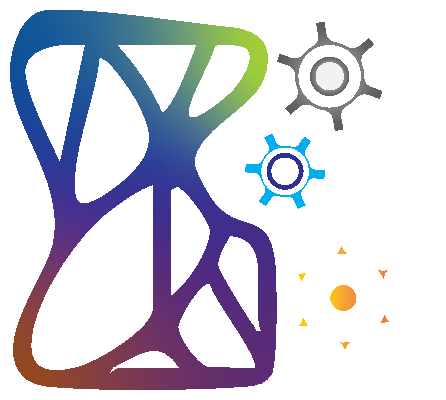
\includegraphics[width=.3\textwidth,height=.45\textheight,keepaspectratio]{Figures/Program symbol.pdf}
  % If you need to crop margins from the image, add: ,trim=20 20 20 20,clip
\end{center}
\vfill

% Bottom meta row
\begin{flushleft}
%{\small \BookAuthor \hspace{1em} -- \hspace{1em} \BookCourse, \BookTerm}
  {\small \BookAuthor}\par
  {\small \BookAuthorTitle}
\end{flushleft}

\begin{flushleft}
  {\small \BookAuthorAffiliation}
\end{flushleft}

\begin{flushright}
  {\small \BookPublisher}
\end{flushright}

\end{titlepage}


\section{Update History}
This textbook is designed for independent study. New chapters and revisions
may be added as the material develops. Major changes are recorded below, with
the most recent change first.

\begin{itemize}
\item[] \textbf{August 18, 2026}: Added Chapter 19 on gradient-based and metaheuristic optimization and Chapter 20 on classification and model selection, with companion scripts and generated figures.
\item[] \textbf{August 17, 2026}: Enlarged code, distributed additional visual explanations, added accessibility support, and introduced algorithms, optimization, and machine-learning Chapters 16--18.
\item[] \textbf{August 17, 2026}: Reorganized Chapters 1--13 for independent study, expanded the visualization applications, and added GeoPandas and geodatasets Chapters 14--15.
\item[] \textbf{October 7, 2025}: \texttt{Data visualization} revised.
\item[] \textbf{October 1, 2025}: \texttt{Data analysis with Pandas} and \texttt{Data visualization} chapters released.
\item[] \textbf{September 25, 2025}: \texttt{Numpy} chapter released.
\item[] \textbf{September 16, 2025}: Added, revised, and reorganized chapters on exceptions, functions, built-in functions, and copying.
\item[] \textbf{September 13, 2025}: Added Chapter 10.
\item[] \textbf{September 9, 2025}: Revised Chapter 8.
\item[] \textbf{September 8, 2025}: Added Chapter 9; revised Chapters 5 and 7.
\item[] \textbf{September 3, 2025}: Added Chapter 8; revised Chapters 5 and 6.
\item[] \textbf{August 25, 2025}: Added Chapter 7.
\item[] \textbf{August 15, 2025}: Added Chapters 5 and 6.
\item[] \textbf{July 2025}: Initial release.
\end{itemize}
\newpage

% =====================
% 00_Title_Imprint.tex — Dedication + imprint page (no images)
% Usage: \newpage% =====================
% 00_Title_Imprint.tex — Dedication + imprint page (no images)
% Usage: \newpage% =====================
% 00_Title_Imprint.tex — Dedication + imprint page (no images)
% Usage: \newpage\input{00_Title_Imprint.tex}
% =====================

\makeatletter
\providecommand{\DedicationTo}{}
\providecommand{\DedicationWhy}{}
\providecommand{\ImprintPublisher}{}
\providecommand{\ImprintCity}{}
\providecommand{\ImprintEdition}{}
\providecommand{\ImprintThanks}{Thank you to the ARC500 cohort for feedback and testing.}
\providecommand{\ImprintCopyrightYears}{2024--2025}
\providecommand{\ImprintHolder}{Junho Chun}
\providecommand{\ImprintLicense}{}
\providecommand{\ImprintISBN}{000-0-00-000000-0}
\makeatother

\thispagestyle{empty}
\vspace*{1.8cm}

% Dedication (top-left)
{\itshape \DedicationTo\par}
\vspace{0.2\baselineskip}
{\itshape \DedicationWhy\par}

\vfill

% Imprint block (bottom-left)
{\small
\textbf{Publisher:} \ImprintPublisher \ImprintCity\par
\ImprintEdition\par
\ImprintThanks\par

\vspace{1.2\baselineskip}
\textbf{Copyright} \ImprintCopyrightYears\ \ImprintHolder\par
\ImprintLicense\par

\vspace{1.2\baselineskip}
\textbf{ISBN:} \ImprintISBN\par
}

% Minimal "barcode-like" rules (no image, purely decorative)
\vspace{1.2cm}
\noindent\begingroup
\setlength{\fboxsep}{0pt}

\par\medskip
{\footnotesize \ImprintISBN}
\endgroup

% =====================

\makeatletter
\providecommand{\DedicationTo}{}
\providecommand{\DedicationWhy}{}
\providecommand{\ImprintPublisher}{}
\providecommand{\ImprintCity}{}
\providecommand{\ImprintEdition}{}
\providecommand{\ImprintThanks}{Thank you to the ARC500 cohort for feedback and testing.}
\providecommand{\ImprintCopyrightYears}{2024--2025}
\providecommand{\ImprintHolder}{Junho Chun}
\providecommand{\ImprintLicense}{}
\providecommand{\ImprintISBN}{000-0-00-000000-0}
\makeatother

\thispagestyle{empty}
\vspace*{1.8cm}

% Dedication (top-left)
{\itshape \DedicationTo\par}
\vspace{0.2\baselineskip}
{\itshape \DedicationWhy\par}

\vfill

% Imprint block (bottom-left)
{\small
\textbf{Publisher:} \ImprintPublisher \ImprintCity\par
\ImprintEdition\par
\ImprintThanks\par

\vspace{1.2\baselineskip}
\textbf{Copyright} \ImprintCopyrightYears\ \ImprintHolder\par
\ImprintLicense\par

\vspace{1.2\baselineskip}
\textbf{ISBN:} \ImprintISBN\par
}

% Minimal "barcode-like" rules (no image, purely decorative)
\vspace{1.2cm}
\noindent\begingroup
\setlength{\fboxsep}{0pt}

\par\medskip
{\footnotesize \ImprintISBN}
\endgroup

% =====================

\makeatletter
\providecommand{\DedicationTo}{}
\providecommand{\DedicationWhy}{}
\providecommand{\ImprintPublisher}{}
\providecommand{\ImprintCity}{}
\providecommand{\ImprintEdition}{}
\providecommand{\ImprintThanks}{Thank you to the ARC500 cohort for feedback and testing.}
\providecommand{\ImprintCopyrightYears}{2024--2025}
\providecommand{\ImprintHolder}{Junho Chun}
\providecommand{\ImprintLicense}{}
\providecommand{\ImprintISBN}{000-0-00-000000-0}
\makeatother

\thispagestyle{empty}
\vspace*{1.8cm}

% Dedication (top-left)
{\itshape \DedicationTo\par}
\vspace{0.2\baselineskip}
{\itshape \DedicationWhy\par}

\vfill

% Imprint block (bottom-left)
{\small
\textbf{Publisher:} \ImprintPublisher \ImprintCity\par
\ImprintEdition\par
\ImprintThanks\par

\vspace{1.2\baselineskip}
\textbf{Copyright} \ImprintCopyrightYears\ \ImprintHolder\par
\ImprintLicense\par

\vspace{1.2\baselineskip}
\textbf{ISBN:} \ImprintISBN\par
}

% Minimal "barcode-like" rules (no image, purely decorative)
\vspace{1.2cm}
\noindent\begingroup
\setlength{\fboxsep}{0pt}

\par\medskip
{\footnotesize \ImprintISBN}
\endgroup

\newpage

\phantomsection
\label{book:toc}
\toc
\newpage

\h*{Reader Roadmap}
\label{reader:roadmap}

This book is organized as a progression from individual instructions to
complete analytical applications. The links below provide five useful entry
routes. If you are new to programming, begin with the first route and continue
in order.

\begin{tcolorbox}[title=Choose a learning route,colframe=orange,colback=white,arc=2mm]
\begin{itemize}
    \item \textbf{Learn Python from the beginning:}
          \booklink{ch:01}{Chapter 1} through \booklink{ch:05}{Chapter 5}.
    \item \textbf{Build reliable, reusable scripts:}
          \booklink{ch:06}{Chapter 6} through \booklink{ch:10}{Chapter 10}.
    \item \textbf{Analyze and communicate data:}
          \booklink{ch:11}{NumPy}, \booklink{ch:12}{pandas}, and
          \booklink{ch:13}{Matplotlib}.
    \item \textbf{Work with geographic data:}
          \booklink{ch:14}{GeoPandas foundations} followed by
          \booklink{ch:15}{geodatasets and applied mapping}.
    \item \textbf{Study computational methods:}
          \booklink{ch:16}{algorithms and efficiency},
          \booklink{ch:17}{numerical optimization}, and
          \booklink{ch:18}{machine-learning foundations}.
\end{itemize}
\end{tcolorbox}

\hh*{Key destinations}

\begin{itemize}
    \item See the \booklink{sec:c13-showcase}{visualization showcase} for a
          compact gallery of analytical plot types.
    \item Follow the \booklink{sec:c13-dashboard}{building-performance
          dashboard} for a longer, practical Matplotlib script.
    \item Use the \booklink{sec:c14-application}{site-access application} to
          connect coordinates, projection, distance, and buffers.
    \item Complete the \booklink{sec:c15-application}{Chicago mapping
          application} to load an educational dataset, align coordinate
          systems, join layers, summarize results, and export a figure.
    \item Compare searches in the
          \booklink{sec:c16-application}{algorithm application}, verify a
          \booklink{sec:c17-application}{bounded optimization model}, and
          evaluate a protected test set in the
          \booklink{sec:c18-application}{machine-learning application}.
\end{itemize}

Every chapter follows the same rhythm: learning outcomes, concepts, syntax
analysis, runnable snippets, visual results where appropriate, guided practice,
solutions, and a checkpoint. Blue text in the PDF is clickable. The footer on
content pages returns to the contents or this roadmap.

\newpage

\part{Part I: Getting Started}
% Part I -- Getting Started
% Chapter 1: Your First Python Program

\h{Your First Python Program}

Python lets you give a computer a clear sequence of instructions. Your goal in
this chapter is simple: install the necessary tools, run a short program, and
understand what appears on the screen. You do not need previous coding
experience.

\begin{NoteBox}
\textbf{Prerequisites.} A Windows or macOS computer, permission to install
software, and a folder where you can save your work.
\end{NoteBox}

\begin{tcolorbox}[title=Learning outcomes,colframe=orange,colback=white,arc=2mm]
After completing this chapter, you should be able to:
\begin{itemize}
    \item explain the difference between the editor, terminal, script, and REPL;
    \item verify that Python 3 is installed;
    \item create and run a Python file in Visual Studio Code;
    \item use \c{print()} to display text and calculation results; and
    \item respond to common setup errors without guessing.
\end{itemize}
\end{tcolorbox}

\hh{How to use this book}

This book is designed for independent study. Work through each chapter in
order. Type the examples instead of only reading them. Small typing mistakes
are normal, and correcting them is part of learning.

You will see five kinds of material:
\begin{itemize}
    \item \textbf{Explanation}: a concept described in plain language.
    \item \textbf{Runnable code}: Python you can type into a file and run.
    \item \textbf{Expected output}: what a correct run should display.
    \item \textbf{Stop and predict}: a question to answer before running code.
    \item \textbf{Practice}: an activity followed by hints and a solution.
\end{itemize}

Do not try to memorize every command. Focus on recognizing what each line asks
Python to do.

\hh{What Python is}

Python is a programming language. A Python program is a text file containing
instructions. Python reads those instructions and performs them in order.

\code{c01_first_print}{python}{
    print("Hello, Python!")
}{A single Python instruction}

The word \c{print} names an action. The parentheses contain the information the
action will use. The quotation marks identify text.

\begin{NoteBox}
\textbf{Stop and predict.} What would you change to display
\c{Hello, ARC500!}?
\end{NoteBox}

\hh{Install Python 3}

Python 3 is the form of the language used in this book.

\hhh*{Windows}
\begin{enumerate}
    \item Visit \url{https://www.python.org/downloads/}.
    \item Download the current Python 3 installer.
    \item Start the installer.
    \item Select \textbf{Add Python to PATH} before choosing Install.
\end{enumerate}

\hhh*{macOS}
\begin{enumerate}
    \item Visit \url{https://www.python.org/downloads/}.
    \item Download and run the current macOS installer.
    \item Complete the installation using the default options.
\end{enumerate}

\hh{Verify the installation}

Open a terminal and enter one of the following commands. Run the commands one
at a time. You only need one of them to work.

\code{c01_verify_python}{bash}{
    python --version
    py --version
    python3 --version
}{Terminal commands for checking the Python version}

A successful response will be similar to:

\code{c01_version_output}{text}{
    Python 3.x.x
}{Example version output; the numbers may differ}

These are terminal commands. Do not type them into a Python file.

\hh{Install Visual Studio Code}

Visual Studio Code, usually called VS Code, is the editor used in this book.
The editor is where you write and save Python instructions.

\begin{enumerate}
    \item Download VS Code from \url{https://code.visualstudio.com/}.
    \item Install and open it.
    \item Select the Extensions icon on the left side.
    \item Search for \textbf{Python} and install the extension published by Microsoft.
    \item Open the Command Palette with \texttt{Ctrl+Shift+P} on Windows or
          \texttt{Cmd+Shift+P} on macOS.
    \item Choose \textbf{Python: Select Interpreter}, then select Python 3.
\end{enumerate}

\hh{Create a study folder}

Create a folder named \texttt{arc500-python}. Inside it, create a folder named
\texttt{chapter01}. Keeping each chapter in its own folder makes your files
easier to find.

In VS Code, choose \textbf{File $\rightarrow$ Open Folder} and open
\texttt{chapter01}. The folder name should appear in the Explorer panel.

\hh{Understand the four working areas}

\begin{itemize}
    \item \textbf{Editor}: the area in VS Code where you write and save code.
    \item \textbf{Terminal}: a text-based area where you enter system commands.
    \item \textbf{Script}: a saved Python file whose name ends in \texttt{.py}.
    \item \textbf{REPL}: an interactive Python prompt that runs one instruction at a time.
\end{itemize}

The terminal and editor are not interchangeable. A command such as
\texttt{python hello.py} belongs in the terminal. An instruction such as
\c{print("Hello")} belongs in a Python file or the REPL.

\hh{Write and run your first script}

In the VS Code Explorer, create a file named \texttt{hello.py}. Type and save:

\code{c01_hello_script}{python}{
    print("Hello, ARC500!")
    print("This is my first Python script.")
}{The complete hello.py script}

Open the VS Code terminal with \textbf{Terminal $\rightarrow$ New Terminal}.
Run the script with the command that works on your computer:

\code{c01_run_script}{bash}{
    python hello.py
}{Run a Python script from the terminal}

On some Windows computers, use \texttt{py hello.py}. On some macOS computers,
use \texttt{python3 hello.py}.

Expected output:

\code{c01_hello_output}{text}{
    Hello, ARC500!
    This is my first Python script.
}{Expected output from hello.py}

Python runs the first instruction and then the second. The output appears in
the same order as the instructions.

\begin{NoteBox}
\textbf{Stop and predict.} If you exchange the two lines in the file, what will
appear first when you run it again?
\end{NoteBox}

\hh{Display a calculation}

The \c{print()} function can display a calculation as well as text.

\code{c01_print_calculations}{python}{
    print(6 + 4)
    print(6 * 4)
    print(24 / 6)
}{Display three calculation results}

Expected output:

\code{c01_calculation_output}{text}{
    10
    24
    4.0
}{Output from the calculations}

Python uses \c{*} for multiplication and \c{/} for division. Chapter 2
explains numbers and arithmetic in more detail.

\hh{Use the interactive prompt}

The REPL is useful when you want to try one instruction without creating a
file. In the terminal, enter \texttt{python}, \texttt{py}, or
\texttt{python3}. A prompt similar to \c{>>>} will appear.

\code{c01_repl_session}{text}{
    >>> print("Testing one instruction")
    Testing one instruction
    >>> 8 * 5
    40
}{A short REPL session}

The \c{>>>} symbol is the prompt. Do not include it in a Python script. Enter
\c{exit()} to leave the REPL.

\hh{Read an error message calmly}

Suppose you accidentally omit a closing quotation mark:

\code{c01_syntax_error}{python}{
    print("Hello)
}{An intentionally incorrect instruction}

Python reports a \c{SyntaxError}. The last line of the message gives the error
type. Look near the indicated line for a missing quotation mark, parenthesis,
or other symbol.

\code{c01_syntax_fixed}{python}{
    print("Hello")
}{The corrected instruction}

\hh{Troubleshooting setup problems}

\begin{itemize}
    \item \textbf{Command not found}: try \texttt{py} or \texttt{python3}. If none
          works, reinstall Python and ensure it is added to PATH.
    \item \textbf{The file does not run}: confirm that the terminal is open in
          the folder containing the file.
    \item \textbf{Old output appears}: save the file before running it.
    \item \textbf{The wrong version appears}: use
          \textbf{Python: Select Interpreter} in VS Code.
    \item \textbf{Nothing appears}: confirm that the file contains \c{print()}
          and that you ran the correct filename.
\end{itemize}

\hh{Practice ladder}

\hhh{Level 0 -- Read and predict}

Write down the expected output before running this code:

\code{c01_practice_level0}{python}{
    print("Start")
    print(3 + 2)
    print("Finish")
}{Predict the output before running the code}

\hhh{Level 1 -- Modify}

Copy the code into \texttt{practice1.py}. Replace the text with your own
subject and learning goal.

\code{c01_practice_level1}{python}{
    print("Subject: Python")
    print("Goal: Run a program successfully")
}{Modify two text values}

\hhh{Level 2 -- Complete}

Write three \c{print()} instructions that produce:

\code{c01_practice_level2_output}{text}{
    ARC500
    20
    Complete
}{Target output for Level 2}

\hhh{Level 3 -- Apply}

Create \texttt{practice3.py}. It should display your name, the text
\texttt{Chapter 1 complete}, and the result of \c{9 * 7}.

\textbf{Hints}
\begin{itemize}
    \item \textbf{Hint 1}: Use one \c{print()} instruction for each line.
    \item \textbf{Hint 2}: Text needs quotation marks; a calculation does not.
    \item \textbf{Hint 3}: Your file should contain three instructions.
\end{itemize}

\hhh{Level 4 -- Challenge}

Use four \c{print()} instructions to produce:

\code{c01_practice_level4_output}{text}{
    Python Study Record
    -------------------
    Chapter: 1
    Status: Complete
}{Target output for the optional challenge}

\hh{Practice solutions}

\textbf{Level 0}

\code{c01_solution_level0}{text}{
    Start
    5
    Finish
}{Level 0 solution}

\textbf{Level 2}

\code{c01_solution_level2}{python}{
    print("ARC500")
    print(12 + 8)
    print("Complete")
}{One solution to Level 2}

\textbf{Level 3}

\code{c01_solution_level3}{python}{
    print("Your Name")
    print("Chapter 1 complete")
    print(9 * 7)
}{One solution to Level 3}

\textbf{Level 4}

\code{c01_solution_level4}{python}{
    print("Python Study Record")
    print("-------------------")
    print("Chapter: 1")
    print("Status: Complete")
}{Solution to Level 4}

\hh{Chapter checkpoint}

Answer without looking back, then check your answers.

\begin{enumerate}
    \item What filename extension identifies a Python script?
    \item Where do you write and save Python code in VS Code?
    \item Where do you enter \texttt{python hello.py}?
    \item What does \c{print()} do?
    \item What symbols identify text in this chapter's examples?
    \item What multiplication symbol does Python use?
    \item What is the purpose of the REPL?
    \item Should \c{>>>} be copied into a Python script?
    \item What should you check first when old output appears?
    \item Name one common cause of a \c{SyntaxError}.
\end{enumerate}

\hh{Checkpoint answers}

\begin{enumerate}
    \item \texttt{.py}.
    \item In the editor.
    \item In the terminal.
    \item It displays information.
    \item Quotation marks.
    \item An asterisk: \c{*}.
    \item It runs one instruction or expression at a time.
    \item No. It is the interactive prompt.
    \item Check that the file was saved and that you ran the correct file.
    \item A missing quotation mark or parenthesis is one possible cause.
\end{enumerate}

\begin{tcolorbox}[title=Chapter summary,colframe=orange,colback=white,arc=2mm]
You installed Python and VS Code, created and ran a Python file, displayed text
and calculations, used the REPL, and corrected a basic syntax mistake. Chapter
2 introduces values, variables, and calculations.
\end{tcolorbox}



\part{Part II: Python Foundations}
% Part II -- Python Foundations
% Chapter 2: Values, Variables, and Calculations

\h{Values, Variables, and Calculations}

A useful program needs information to work with. That information may be a
number, a piece of text, or a yes-or-no value. In this chapter, you will learn
how Python represents these values, how to give them clear names, and how to
use them in calculations.

\begin{NoteBox}
\textbf{Prerequisites.} You should be able to create, save, and run a Python
file and use \c{print()}.
\end{NoteBox}

\begin{tcolorbox}[title=Learning outcomes,colframe=orange,colback=white,arc=2mm]
After completing this chapter, you should be able to:
\begin{itemize}
    \item recognize integers, floating-point numbers, strings, booleans, and \c{None};
    \item assign values to clearly named variables;
    \item perform and organize arithmetic calculations;
    \item read text with \c{input()} and convert it to a number; and
    \item produce readable output with an f-string.
\end{itemize}
\end{tcolorbox}

\hh{Values and types}

A \emph{value} is one piece of information. Every value has a \emph{type}. The
type tells Python what kind of information the value represents and which
operations make sense for it.

\begin{lstlisting}[
    language=python,
    style=block,
    caption={Five basic Python values},
    label={c02_basic_values},
    captionpos=b
]
print(4)
print(3.5)
print("Studio")
print(True)
print(None)
\end{lstlisting}

These values have different types:
\begin{itemize}
    \item \c{4} is an integer, written \c{int}.
    \item \c{3.5} is a floating-point number, written \c{float}.
    \item \c{"Studio"} is a string, written \c{str}.
    \item \c{True} is a boolean, written \c{bool}.
    \item \c{None} represents the absence of a value.
\end{itemize}

Use \c{type()} when you want Python to report a value's type.

\begin{lstlisting}[
    language=python,
    style=block,
    caption={Inspect three value types},
    label={c02_type_check},
    captionpos=b
]
print(type(4))
print(type(3.5))
print(type("Studio"))
\end{lstlisting}

\begin{NoteBox}
\textbf{Stop and predict.} What type will Python report for \c{"4"}? Notice
that quotation marks change a number into text.
\end{NoteBox}

\hh{Variables give values names}

A variable is a name connected to a value. The equals sign assigns the value
on the right to the name on the left.

\begin{lstlisting}[
    language=python,
    style=block,
    caption={Assign and display three variables},
    label={c02_first_variables},
    captionpos=b
]
room_name = "Studio"
width_m = 6.0
length_m = 8.0

print(room_name)
print(width_m)
print(length_m)
\end{lstlisting}

Read \c{width_m = 6.0} as ``assign the value 6.0 to \c{width_m}.'' The equals
sign performs assignment here; it is not asking a mathematical question.

Use names that explain the value:
\begin{itemize}
    \item begin with a letter or underscore;
    \item use letters, numbers, and underscores only;
    \item use lowercase words separated by underscores; and
    \item include units when they prevent confusion.
\end{itemize}

Names such as \c{wall_height_m} and \c{area_m2} are clearer than \c{x} and
\c{result}.

\hh{Variables can be reassigned}

A variable can receive a new value later.

\begin{lstlisting}[
    language=python,
    style=block,
    caption={Reassign a variable},
    label={c02_reassignment},
    captionpos=b
]
floor_count = 3
print(floor_count)

floor_count = 4
print(floor_count)
\end{lstlisting}

Expected output:

\begin{lstlisting}[
    language=text,
    style=block,
    caption={Output after reassignment},
    label={c02_reassignment_output},
    captionpos=b
]
3
4
\end{lstlisting}

Reassignment does not change the earlier output. It changes which value the
name refers to from that point forward.

\hh{Work with numbers}

Python uses familiar arithmetic operators.

\begin{center}
\begin{tabular}{lll}
\textbf{Operation} & \textbf{Operator} & \textbf{Example} \\
Addition & \c{+} & \c{8 + 2} \\
Subtraction & \c{-} & \c{8 - 2} \\
Multiplication & \c{*} & \c{8 * 2} \\
Division & \c{/} & \c{8 / 2} \\
Floor division & \c{//} & \c{9 // 2} \\
Exponentiation & \c{**} & \c{3 ** 2} \\
\end{tabular}
\end{center}

Parentheses make the intended order clear.

\begin{lstlisting}[
    language=python,
    style=block,
    caption={Calculate area and volume},
    label={c02_arithmetic},
    captionpos=b
]
width_m = 6.0
length_m = 8.0
height_m = 3.2

area_m2 = width_m * length_m
volume_m3 = area_m2 * height_m

print(area_m2)
print(volume_m3)
\end{lstlisting}

\begin{NoteBox}
\textbf{Stop and predict.} If \c{width_m} changes to \c{7.0}, which results
will change? Make a prediction before running the revised code.
\end{NoteBox}

\hh{Control calculation order}

Python follows standard arithmetic precedence. Multiplication and division
occur before addition and subtraction. Parentheses let you state the intended
order directly.

\begin{lstlisting}[
    language=python,
    style=block,
    caption={Parentheses change calculation order},
    label={c02_precedence},
    captionpos=b
]
result_a = 4 + 3 * 2
result_b = (4 + 3) * 2

print(result_a)
print(result_b)
\end{lstlisting}

Expected output:

\begin{lstlisting}[
    language=text,
    style=block,
    caption={Results with and without parentheses},
    label={c02_precedence_output},
    captionpos=b
]
10
14
\end{lstlisting}

Use parentheses when a reader might otherwise need to stop and check the
order.

\hh{Work with strings}

A string is text inside quotation marks. Single and double quotation marks
both create strings.

\begin{lstlisting}[
    language=python,
    style=block,
    caption={Create two strings},
    label={c02_strings},
    captionpos=b
]
room_name = "Lecture Room"
level_name = 'Second Floor'

print(room_name)
print(level_name)
\end{lstlisting}

Choose one quotation style and use it consistently. A string can contain
spaces, punctuation, and digits. The digits in \c{"Room 204"} are still text.

Strings can be joined with \c{+}.

\begin{lstlisting}[
    language=python,
    style=block,
    caption={Join two strings},
    label={c02_string_join},
    captionpos=b
]
room_name = "Studio"
message = "Room: " + room_name
print(message)
\end{lstlisting}

For messages containing numbers, an f-string is usually clearer than joining
many converted values.

\hh{Read input from the student}

The \c{input()} function displays a prompt, waits for the user to type, and
returns the response as a string.

\begin{lstlisting}[
    language=python,
    style=block,
    caption={Read and display text input},
    label={c02_text_input},
    captionpos=b
]
room_name = input("Room name: ")
print("You entered: " + room_name)
\end{lstlisting}

Even when a user types digits, \c{input()} returns text. Convert the response
before using it in arithmetic.

\begin{lstlisting}[
    language=python,
    style=block,
    caption={Convert input text to a floating-point number},
    label={c02_numeric_input},
    captionpos=b
]
width_text = input("Width in meters: ")
width_m = float(width_text)

print(width_m * 2)
\end{lstlisting}

You can combine reading and conversion when the shorter form remains clear.

\begin{lstlisting}[
    language=python,
    style=block,
    caption={Read two dimensions and calculate area},
    label={c02_direct_conversion},
    captionpos=b
]
width_m = float(input("Width in meters: "))
length_m = float(input("Length in meters: "))
area_m2 = width_m * length_m

print(area_m2)
\end{lstlisting}

If the user types text that cannot be converted, Python reports a
\c{ValueError}. Chapter 8 will show how to handle that error. For now, enter a
valid number when a prompt requests one.

\hh{Format output with f-strings}

An f-string places values inside a readable message. Begin the string with
\c{f} and place variable names inside braces.

\begin{lstlisting}[
    language=python,
    style=block,
    caption={Insert values into an f-string},
    label={c02_first_fstring},
    captionpos=b
]
room_name = "Studio"
area_m2 = 48.0

print(f"{room_name} area: {area_m2} m2")
\end{lstlisting}

Use a format specification to control decimal places.

\begin{lstlisting}[
    language=python,
    style=block,
    caption={Display a number with two decimal places},
    label={c02_decimal_format},
    captionpos=b
]
width_m = 5.75
length_m = 7.2
area_m2 = width_m * length_m

print(f"Area: {area_m2:.2f} m2")
\end{lstlisting}

The specification \c{:.2f} displays a floating-point value with two digits
after the decimal point. It changes the displayed form, not the stored value.

\hh{Use comments to explain intent}

A comment begins with \c{#}. Python ignores the comment when the program runs.
Use comments to explain an assumption or decision.

\begin{lstlisting}[
    language=python,
    style=block,
    caption={A comment records an important assumption},
    label={c02_comments},
    captionpos=b
]
# Dimensions are measured in meters.
width_m = 5.75
length_m = 7.2

area_m2 = width_m * length_m
print(f"Area: {area_m2:.2f} m2")
\end{lstlisting}

Avoid comments that merely repeat the code. A comment should add information
that the names and operations do not already communicate.

\hh{Common mistakes}

\hhh{Using a variable before assigning it}

\begin{lstlisting}[
    language=python,
    style=block,
    caption={This intentionally produces a NameError},
    label={c02_name_error},
    captionpos=b
]
print(area_m2)
\end{lstlisting}

Assign \c{area_m2} before trying to use it.

\hhh{Mixing text and numbers with plus}

\begin{lstlisting}[
    language=python,
    style=block,
    caption={This intentionally produces a TypeError},
    label={c02_type_error},
    captionpos=b
]
area_m2 = 48.0
print("Area: " + area_m2)
\end{lstlisting}

Use an f-string instead:

\begin{lstlisting}[
    language=python,
    style=block,
    caption={Use an f-string to combine text and a number},
    label={c02_type_error_fixed},
    captionpos=b
]
area_m2 = 48.0
print(f"Area: {area_m2} m2")
\end{lstlisting}

\hhh{Using an unclear name}

\begin{lstlisting}[
    language=python,
    style=block,
    caption={Valid code with unclear names},
    label={c02_unclear_names},
    captionpos=b
]
a = 6.0
b = 8.0
c = a * b
\end{lstlisting}

Prefer \c{width_m}, \c{length_m}, and \c{area_m2}. Clear names reduce the
amount of explanation a reader needs.

\hh{Practice ladder}

\hhh{Level 0 -- Read and predict}

Predict the output before running the code.

\begin{lstlisting}[
    language=python,
    style=block,
    caption={Predict a calculation result},
    label={c02_practice_level0},
    captionpos=b
]
width_m = 4.0
length_m = 6.0
area_m2 = width_m * length_m
print(area_m2)
\end{lstlisting}

\hhh{Level 1 -- Modify}

Run the code above. Change the width and length to two different values. Check
the result by hand, then run the code again.

\hhh{Level 2 -- Complete}

Replace \c{...} with the missing expression so the program calculates
perimeter. Complete the line before you run the program.

\begin{lstlisting}[
    language=python,
    style=block,
    caption={Complete one missing expression},
    label={c02_practice_level2},
    captionpos=b
]
width_m = 5.0
length_m = 9.0
perimeter_m = ...  # Replace ... with the perimeter calculation.

print(f"Perimeter: {perimeter_m:.1f} m")
\end{lstlisting}

\hhh{Level 3 -- Apply}

Write a program that asks for width, length, and height. Calculate area and
volume, then display both results with two decimal places.

\textbf{Hints}
\begin{itemize}
    \item \textbf{Hint 1}: Use \c{float(input(...))} three times.
    \item \textbf{Hint 2}: Calculate area before volume.
    \item \textbf{Hint 3}: Volume equals area multiplied by height.
\end{itemize}

\hhh{Level 4 -- Challenge}

Extend Level 3 by calculating the difference between the length and width.
Display a clear sentence describing the difference.

\hh{Practice solutions}

\textbf{Level 0:} The output is \c{24.0}.

\textbf{Level 2}

\begin{lstlisting}[
    language=python,
    style=block,
    caption={One solution to Level 2},
    label={c02_solution_level2},
    captionpos=b
]
width_m = 5.0
length_m = 9.0
perimeter_m = 2 * (width_m + length_m)

print(f"Perimeter: {perimeter_m:.1f} m")
\end{lstlisting}

\textbf{Level 3}

\begin{lstlisting}[
    language=python,
    style=block,
    caption={One solution to Level 3},
    label={c02_solution_level3},
    captionpos=b
]
width_m = float(input("Width in meters: "))
length_m = float(input("Length in meters: "))
height_m = float(input("Height in meters: "))

area_m2 = width_m * length_m
volume_m3 = area_m2 * height_m

print(f"Area: {area_m2:.2f} m2")
print(f"Volume: {volume_m3:.2f} m3")
\end{lstlisting}

\textbf{Level 4 addition}

\begin{lstlisting}[
    language=python,
    style=block,
    caption={One solution that extends Level 3},
    label={c02_solution_level4},
    captionpos=b
]
width_m = float(input("Width in meters: "))
length_m = float(input("Length in meters: "))
height_m = float(input("Height in meters: "))

area_m2 = width_m * length_m
volume_m3 = area_m2 * height_m
difference_m = length_m - width_m

print(f"Area: {area_m2:.2f} m2")
print(f"Volume: {volume_m3:.2f} m3")
print(f"Length minus width: {difference_m:.2f} m")
\end{lstlisting}

\hh{Chapter checkpoint}

\begin{enumerate}
    \item What is the difference between \c{4} and \c{"4"}?
    \item What does the assignment operator do?
    \item Why is \c{area_m2} clearer than \c{x}?
    \item Which operator performs multiplication?
    \item Why might you use parentheses in a calculation?
    \item What type does \c{input()} return?
    \item How do you convert \c{"3.5"} to a number?
    \item What does the \c{f} before an f-string mean for its braces?
    \item What does \c{:.2f} control?
    \item What symbol begins a comment?
\end{enumerate}

\hh{Checkpoint answers}

\begin{enumerate}
    \item \c{4} is an integer; \c{"4"} is a string.
    \item It connects a name to a value.
    \item The name describes the quantity and its unit.
    \item \c{*}.
    \item To make the intended order clear or change the normal order.
    \item A string.
    \item Use \c{float("3.5")}.
    \item Values or expressions inside braces are inserted into the text.
    \item The displayed number of decimal places.
    \item \c{#}.
\end{enumerate}

\begin{tcolorbox}[title=Chapter summary,colframe=orange,colback=white,arc=2mm]
Values have types. Variables give values meaningful names. Python can perform
calculations with numeric variables, read responses with \c{input()}, convert
text to numbers, and insert results into f-strings. Chapter 3 shows how to
organize several related values in collections.
\end{tcolorbox}



% Part II -- Python Foundations
% Chapter 3: Organizing Data

\h{Organizing Data}
\label{ch:03}

A single variable holds one value. Many tasks require several related values:
room names, floor areas, material codes, or measurements. Python provides
collections for storing these values together. This chapter introduces four
collections and explains when each one is useful.

\begin{NoteBox}
\textbf{Prerequisites.} You should understand values, variables, assignment,
basic types, and \c{print()}.
\end{NoteBox}

\begin{tcolorbox}[title=Learning outcomes,colframe=orange,colback=white,arc=2mm]
After completing this chapter, you should be able to:
\begin{itemize}
    \item create, read, and modify a list;
    \item store labeled values in a dictionary;
    \item use a tuple for a fixed record and a set for unique values;
    \item test whether a collection contains a value; and
    \item choose a suitable collection for a simple situation.
\end{itemize}
\end{tcolorbox}

\hh{Why collections are useful}

Without a collection, four room names require four variables.

\begin{lstlisting}[
    language=python,
    style=block,
    caption={Four separate variables},
    label={c03_separate_names},
    captionpos=b
]
room_1 = "Lobby"
room_2 = "Studio"
room_3 = "Office"
room_4 = "Cafe"
\end{lstlisting}

A list stores the same information under one name.

\begin{lstlisting}[
    language=python,
    style=block,
    caption={Store several room names in one list},
    label={c03_first_list},
    captionpos=b
]
room_names = ["Lobby", "Studio", "Office", "Cafe"]
print(room_names)
\end{lstlisting}

The square brackets identify a list. Commas separate its items.

\begin{ExplainBox}{A collection encodes a relationship among values}
Putting values together is not only a storage convenience. The collection
type states what relationship the program relies on. A list says that order
and position matter. A dictionary says that each value is retrieved through a
meaningful key. A tuple says that a small ordered record should not be changed
in place. A set says that membership and uniqueness matter more than position.
Choosing the wrong relationship produces awkward code even when the values
themselves are correct.
\end{ExplainBox}

Collections also have behavioral properties:
\begin{itemize}
    \item \textbf{ordered} means iteration follows a defined sequence;
    \item \textbf{mutable} means the existing object can be changed in place;
    \item \textbf{indexed} means a position such as \c{0} selects an item;
    \item \textbf{keyed} means a meaningful key selects a value;
    \item \textbf{unique} means duplicate members collapse into one member.
\end{itemize}

These properties are independent questions. A list is ordered, mutable, and
indexed, while a set is mutable and unique but not position-indexed. Chapter 9
will show why mutability also affects assignment and copying.

\hh{Create lists}

A list is an ordered, changeable collection. Its items may be numbers, strings,
booleans, or other values.

\begin{lstlisting}[
    language=python,
    style=block,
    caption={Create four lists},
    label={c03_list_examples},
    captionpos=b
]
floor_numbers = [1, 2, 3, 4]
room_areas_m2 = [24.0, 35.5, 18.0]
status_labels = ["Open", "Closed", "Review"]
empty_list = []

print(floor_numbers)
print(room_areas_m2)
print(status_labels)
print(empty_list)
\end{lstlisting}

Use \c{len()} to find the number of items.

\begin{lstlisting}[
    language=python,
    style=block,
    caption={Count list items},
    label={c03_list_length},
    captionpos=b
]
room_names = ["Lobby", "Studio", "Office", "Cafe"]
print(len(room_names))
\end{lstlisting}

\hh{Read list items by index}

Each item has a position called an \emph{index}. Python begins counting at
zero.

\begin{lstlisting}[
    language=python,
    style=block,
    caption={Read list items by position},
    label={c03_list_index},
    captionpos=b
]
room_names = ["Lobby", "Studio", "Office", "Cafe"]

print(room_names[0])
print(room_names[1])
print(room_names[-1])
\end{lstlisting}

Expected output:

\begin{lstlisting}[
    language=text,
    style=block,
    caption={List indexing output},
    label={c03_list_index_output},
    captionpos=b
]
Lobby
Studio
Cafe
\end{lstlisting}

An index of \c{-1} means the last item.

\begin{NoteBox}
\textbf{Stop and predict.} What will \c{room_names[2]} display? What is the
largest valid positive index for this four-item list?
\end{NoteBox}

An index outside the list produces an \c{IndexError}.

\hh{Select part of a list}

A slice selects a range of items. The stop position is not included.

\begin{lstlisting}[
    language=python,
    style=block,
    caption={Select list slices},
    label={c03_list_slice},
    captionpos=b
]
levels = ["B1", "L1", "L2", "L3", "Roof"]

print(levels[1:4])
print(levels[:2])
print(levels[3:])
\end{lstlisting}

Expected output:

\begin{lstlisting}[
    language=text,
    style=block,
    caption={Three list slices},
    label={c03_list_slice_output},
    captionpos=b
]
['L1', 'L2', 'L3']
['B1', 'L1']
['L3', 'Roof']
\end{lstlisting}

\begin{SyntaxBox}{A slice describes a half-open range}
Lists, strings, and tuples are all sequences -- ordered collections that
support this same slicing pattern. The pattern is \c{sequence[start:stop]}.
Python includes the item at \c{start} and stops before \c{stop}. Omitting
\c{start} means ``from the beginning''; omitting \c{stop} means ``through the
end.''
\end{SyntaxBox}

\bookfigure[0.88\textwidth]{Figures/List/List_operator.pdf}
{Visual guide to list indexing, slicing, and common list operations.}
{fig:ch03-list-operations}

\hh{Change a list}

Lists are mutable, which means their contents can change.

\begin{lstlisting}[
    language=python,
    style=block,
    caption={Replace one item and append another},
    label={c03_modify_list},
    captionpos=b
]
room_names = ["Lobby", "Studio", "Office"]

room_names[2] = "Meeting Room"
room_names.append("Cafe")

print(room_names)
\end{lstlisting}

Common list methods include:
\begin{itemize}
    \item \c{append(value)}: add one item at the end;
    \item \c{insert(index, value)}: add an item at a chosen position;
    \item \c{remove(value)}: remove the first matching value;
    \item \c{pop()}: remove and return the last item; and
    \item \c{clear()}: remove all items.
\end{itemize}

\begin{lstlisting}[
    language=python,
    style=block,
    caption={Insert, remove, and pop list items},
    label={c03_list_methods},
    captionpos=b
]
materials = ["Concrete", "Steel"]

materials.insert(1, "Timber")
materials.remove("Steel")
removed_item = materials.pop()

print(materials)
print(removed_item)
\end{lstlisting}

After \c{remove("Steel")}, the list contains \c{"Concrete"} and
\c{"Timber"}. Then \c{pop()} removes and returns \c{"Timber"}.

\hh{Check membership}

The \c{in} operator asks whether a collection contains a value. The result is
\c{True} or \c{False}.

\begin{lstlisting}[
    language=python,
    style=block,
    caption={Check list membership},
    label={c03_list_membership},
    captionpos=b
]
materials = ["Concrete", "Timber", "Glass"]

print("Timber" in materials)
print("Brick" in materials)
\end{lstlisting}

Membership checks are case-sensitive. \c{"timber"} and \c{"Timber"} are
different strings.

\hh{Create dictionaries}

A dictionary stores key--value pairs. Each key is a label used to retrieve its
value. Curly braces identify a dictionary, and a colon separates each key from
its value.

\begin{lstlisting}[
    language=python,
    style=block,
    caption={A dictionary describing one room},
    label={c03_first_dictionary},
    captionpos=b
]
room = {
    "name": "Studio",
    "area_m2": 48.0,
    "level": 2
}

print(room)
\end{lstlisting}

Use a key inside square brackets to read a value.

\begin{lstlisting}[
    language=python,
    style=block,
    caption={Read dictionary values by key},
    label={c03_dictionary_access},
    captionpos=b
]
room = {
    "name": "Studio",
    "area_m2": 48.0,
    "level": 2
}

print(room["name"])
print(room["area_m2"])
\end{lstlisting}

Unlike list indexes, dictionary keys communicate what the values mean.

\bookfigure[0.86\textwidth]{Figures/Dictionary/Dictionary.pdf}
{A dictionary connects descriptive keys to values rather than relying on numerical positions.}
{fig:ch03-dictionary-model}

\begin{TryBox}{Choose a collection before writing code}
For each case, choose a list, dictionary, tuple, or set and justify the choice:
an ordered room schedule; one room's named properties; an immutable RGB color;
and the unique material names found in a model. Then create one small example
of each collection in Python.
\end{TryBox}

\hh{Update a dictionary}

Assign to an existing key to replace its value. Assign to a new key to add a
new pair.

\begin{lstlisting}[
    language=python,
    style=block,
    caption={Replace one value and add another},
    label={c03_dictionary_update},
    captionpos=b
]
room = {
    "name": "Studio",
    "area_m2": 48.0
}

room["area_m2"] = 50.5
room["level"] = 2

print(room)
\end{lstlisting}

Use \c{pop(key)} to remove a pair and return its value.

\begin{lstlisting}[
    language=python,
    style=block,
    caption={Remove a dictionary pair},
    label={c03_dictionary_pop},
    captionpos=b
]
room = {
    "name": "Studio",
    "area_m2": 50.5,
    "level": 2
}

removed_level = room.pop("level")
print(removed_level)
print(room)
\end{lstlisting}

\hh{Use safe dictionary lookup}

Square-bracket lookup produces a \c{KeyError} when the requested key is
missing. The \c{get()} method can return a default value instead.

\begin{lstlisting}[
    language=python,
    style=block,
    caption={Use get for a key that may be missing},
    label={c03_dictionary_get},
    captionpos=b
]
room = {
    "name": "Studio",
    "area_m2": 50.5
}

print(room.get("name"))
print(room.get("occupancy", "Not recorded"))
\end{lstlisting}

Use square brackets when a key must exist. Use \c{get()} when a missing value
has a reasonable default.

Dictionary membership checks keys.

\begin{lstlisting}[
    language=python,
    style=block,
    caption={Check whether dictionary keys exist},
    label={c03_dictionary_membership},
    captionpos=b
]
room = {"name": "Studio", "area_m2": 50.5}

print("name" in room)
print("level" in room)
\end{lstlisting}

\hh{Use tuples for fixed records}

A tuple is an ordered collection that cannot be changed after creation.
Parentheses identify a tuple.

\begin{lstlisting}[
    language=python,
    style=block,
    caption={A fixed two-coordinate record},
    label={c03_first_tuple},
    captionpos=b
]
point_xy = (12.5, 8.0)

print(point_xy[0])
print(point_xy[1])
\end{lstlisting}

A tuple is useful when the number and meaning of its positions should remain
fixed. Use a list when items need to be added, removed, or replaced.

\hh{Use sets for unique values}

A set stores unique values. Repeated values are removed automatically. Sets do
not provide list-style positional indexing.

\begin{lstlisting}[
    language=python,
    style=block,
    caption={A set removes a repeated value},
    label={c03_first_set},
    captionpos=b
]
materials = {"Steel", "Glass", "Steel", "Concrete"}
print(materials)
\end{lstlisting}

The displayed order may vary. Use \c{set()} to create an empty set because
empty curly braces create an empty dictionary.

\begin{lstlisting}[
    language=python,
    style=block,
    caption={Add an item and check set membership},
    label={c03_set_membership},
    captionpos=b
]
materials = {"Steel", "Glass", "Concrete"}

materials.add("Timber")
print("Timber" in materials)
print(len(materials))
\end{lstlisting}

\hh{Choose a collection}

\begin{center}
\begin{tabular}{lll}
\textbf{Collection} & \textbf{Main feature} & \textbf{Use when} \\
List & Ordered and changeable & Position and sequence matter \\
Dictionary & Labeled key--value pairs & Values need meaningful labels \\
Tuple & Ordered and fixed & A small record should not change \\
Set & Unique values & Duplicates should be removed \\
\end{tabular}
\end{center}

Ask two questions before choosing: Does order matter? Does each value need a
label? These questions usually narrow the choice quickly.

Then test the choice against the operations the program must perform:
\begin{enumerate}
    \item Must duplicate values be preserved? Use a list or tuple, not a set.
    \item Must an item be retrieved by a descriptive name? Use a dictionary.
    \item Must insertion, deletion, or replacement occur in place? Use a
          mutable list, dictionary, or set.
    \item Is the object a fixed coordinate or record whose positions have
          stable meanings? A tuple may communicate that constraint.
    \item Is the central question ``has this value appeared?'' A set expresses
          that membership question directly.
\end{enumerate}

For example, room names in walking order belong in a list; room areas looked
up by room name belong in a dictionary; a fixed \c{(x, y)} coordinate can be a
tuple; and the unique material categories present in a dataset belong in a
set. The values may look similar, but the required relationships differ.

\hh{Common mistakes}

\begin{itemize}
    \item \textbf{Starting at index 1}: the first list index is 0.
    \item \textbf{Using a missing key}: check the key or use \c{get()}.
    \item \textbf{Expecting a set to preserve position}: sets are not indexed sequences.
    \item \textbf{Creating an empty set with curly braces}: use \c{set()}.
    \item \textbf{Changing a tuple}: create a new tuple instead.
\end{itemize}

\hh{Practice ladder}

\hhh{Level 0 -- Read}

\begin{lstlisting}[
    language=python,
    style=block,
    caption={Predict two list lookups},
    label={c03_practice_level0},
    captionpos=b
]
levels = ["B1", "L1", "L2"]
print(levels[0])
print(levels[-1])
\end{lstlisting}

\hhh{Level 1 -- Modify}

Add two room names to the list, replace the first item, and print the result.

\begin{lstlisting}[
    language=python,
    style=block,
    caption={Starting list for modification},
    label={c03_practice_level1},
    captionpos=b
]
rooms = ["Lobby", "Studio"]
print(rooms)
\end{lstlisting}

\hhh{Level 2 -- Complete}

Replace each \c{...} with a value to complete a dictionary that stores a room
name, area, and level. Then display only the name and area.

\begin{lstlisting}[
    language=python,
    style=block,
    caption={Complete three dictionary values},
    label={c03_practice_level2},
    captionpos=b
]
room = {
    "name": ...,
    "area_m2": ...,
    "level": ...
}

print(room["name"])
print(room["area_m2"])
\end{lstlisting}

\hhh{Level 3 -- Apply}

Create:
\begin{enumerate}
    \item a list containing four material names;
    \item a dictionary containing one material's name and unit cost; and
    \item a set created from a list that contains at least one duplicate.
\end{enumerate}
Display each collection and its length.

\textbf{Hints}
\begin{itemize}
    \item \textbf{Hint 1}: Use square brackets for the list.
    \item \textbf{Hint 2}: Use descriptive string keys in the dictionary.
    \item \textbf{Hint 3}: Pass the duplicate-containing list to \c{set()}.
\end{itemize}

\hhh{Level 4 -- Challenge}

Create a dictionary containing a room's name and a list of three finish
materials. Add a fourth material to the nested list and display the result.

\hh{Practice solutions}

\textbf{Level 0:} The output is \c{B1}, then \c{L2}.

\textbf{Level 2}

\begin{lstlisting}[
    language=python,
    style=block,
    caption={One solution to Level 2},
    label={c03_solution_level2},
    captionpos=b
]
room = {
    "name": "Seminar Room",
    "area_m2": 32.0,
    "level": 3
}

print(room["name"])
print(room["area_m2"])
\end{lstlisting}

\textbf{Level 3 -- one possible solution}

\begin{lstlisting}[
    language=python,
    style=block,
    caption={One solution to Level 3},
    label={c03_solution_level3},
    captionpos=b
]
materials = ["Concrete", "Steel", "Glass", "Timber"]
material_cost = {"name": "Concrete", "cost_per_m2": 42.0}

repeated_names = ["Steel", "Glass", "Steel", "Timber"]
unique_materials = set(repeated_names)

print(materials, len(materials))
print(material_cost, len(material_cost))
print(unique_materials, len(unique_materials))
\end{lstlisting}

\textbf{Level 4}

\begin{lstlisting}[
    language=python,
    style=block,
    caption={One solution to Level 4},
    label={c03_solution_level4},
    captionpos=b
]
room = {
    "name": "Studio",
    "finishes": ["Concrete", "Paint", "Timber"]
}

room["finishes"].append("Glass")
print(room)
\end{lstlisting}

\hh{Chapter checkpoint}

\begin{enumerate}
    \item Which brackets identify a list?
    \item What is the index of the first list item?
    \item What does a negative index of \c{-1} select?
    \item Does a slice include its stop position?
    \item Which method adds one item to the end of a list?
    \item What two parts make up a dictionary pair?
    \item When is \c{get()} useful?
    \item Why might you choose a tuple instead of a list?
    \item What happens to duplicate values in a set?
    \item How do you create an empty set?
\end{enumerate}

\hh{Checkpoint answers}

\begin{enumerate}
    \item Square brackets.
    \item Zero.
    \item The last item.
    \item No.
    \item \c{append()}.
    \item A key and a value.
    \item When a key may be missing and a default is appropriate.
    \item A tuple communicates that the record should remain fixed.
    \item They are removed.
    \item Use \c{set()}.
\end{enumerate}

\begin{tcolorbox}[title=Chapter summary,colframe=orange,colback=white,arc=2mm]
Lists store ordered, changeable items. Dictionaries connect labels to values.
Tuples are useful for fixed records, and sets store unique values. Chapter 4
uses boolean expressions and conditions to make decisions with these values.
\end{tcolorbox}


% Part II -- Python Foundations
% Chapter 4: Booleans and Decisions

\h{Booleans and Decisions}

Programs often need to choose between actions. A room may pass or fail a size
check. A value may be inside or outside a permitted range. Python represents
these yes-or-no results with booleans and uses conditional statements to choose
which instructions to run.

\begin{NoteBox}
\textbf{Prerequisites.} You should understand variables, numbers, strings,
lists, dictionaries, membership, and basic input conversion.
\end{NoteBox}

\begin{tcolorbox}[title=Learning outcomes,colframe=orange,colback=white,arc=2mm]
After completing this chapter, you should be able to:
\begin{itemize}
    \item create boolean values with comparisons;
    \item combine conditions with \c{and}, \c{or}, and \c{not};
    \item write \c{if}, \c{elif}, and \c{else} statements;
    \item use membership tests in decisions; and
    \item trace which branch of a conditional statement will run.
\end{itemize}
\end{tcolorbox}

\hh{Boolean values}

Python has two boolean values: \c{True} and \c{False}. Their capital letters
matter.

\code{c04_boolean_values}{python}{
    is_accessible = True
    needs_review = False

    print(is_accessible)
    print(needs_review)
}{Store and display boolean values}

Boolean values usually come from questions expressed as comparisons.

\hh{Compare values}

Comparison operators produce \c{True} or \c{False}.

\begin{center}
\begin{tabular}{lll}
\textbf{Question} & \textbf{Operator} & \textbf{Example} \\
Equal to & \c{==} & \c{area_m2 == 30} \\
Not equal to & \c{!=} & \c{level != 1} \\
Greater than & \c{>} & \c{width_m > 3} \\
Less than & \c{<} & \c{width_m < 3} \\
Greater than or equal to & \c{>=} & \c{area_m2 >= 20} \\
Less than or equal to & \c{<=} & \c{area_m2 <= 40} \\
\end{tabular}
\end{center}

\code{c04_comparisons}{python}{
    area_m2 = 32.0

    print(area_m2 > 20.0)
    print(area_m2 == 32.0)
    print(area_m2 < 25.0)
}{Three comparisons}

Expected output:

\code{c04_comparisons_output}{text}{
    True
    True
    False
}{Comparison results}

Do not confuse \c{=} with \c{==}. A single equals sign assigns a value. Two
equals signs compare two values.

\begin{NoteBox}
\textbf{Stop and predict.} What are the results of \c{5 >= 5}, \c{5 > 5}, and
\c{"Studio" == "studio"}?
\end{NoteBox}

\hh{Check a range}

Python can express a range as one chained comparison.

\code{c04_chained_comparison}{python}{
    area_m2 = 32.0
    is_medium = 20.0 <= area_m2 <= 40.0

    print(is_medium)
}{Check whether a value is inside a range}

The expression is true when both boundaries are satisfied.

\hh{Combine conditions with and}

The \c{and} operator is true only when both conditions are true.

\code{c04_and_operator}{python}{
    width_m = 4.0
    length_m = 7.0

    dimensions_positive = width_m > 0 and length_m > 0
    print(dimensions_positive)
}{Require two conditions}

Use \c{and} when every requirement must be satisfied.

\hh{Combine alternatives with or}

The \c{or} operator is true when at least one condition is true.

\code{c04_or_operator}{python}{
    room_type = "Studio"

    is_work_space = room_type == "Studio" or room_type == "Office"
    print(is_work_space)
}{Accept either of two values}

Use \c{or} when one of several alternatives is enough.

\hh{Reverse a boolean with not}

The \c{not} operator reverses a boolean result.

\code{c04_not_operator}{python}{
    needs_review = False
    is_approved = not needs_review

    print(is_approved)
}{Reverse a boolean value}

Keep combined conditions short. A named boolean such as \c{is_approved} is
often easier to read than a long expression repeated several times.

\hh{Use membership conditions}

The \c{in} operator works with collections and returns a boolean.

\code{c04_membership_condition}{python}{
    allowed_types = ["Studio", "Office", "Classroom"]
    room_type = "Studio"

    is_allowed = room_type in allowed_types
    print(is_allowed)
}{Check whether a value is in a list}

Use \c{not in} to ask the opposite question.

\code{c04_not_in}{python}{
    allowed_types = ["Studio", "Office", "Classroom"]
    room_type = "Storage"

    print(room_type not in allowed_types)
}{Check that a value is absent}

\hh{Make a decision with if}

An \c{if} statement runs an indented block only when its condition is true.

\code{c04_first_if}{python}{
    area_m2 = 32.0

    if area_m2 >= 20.0:
        print("Area requirement passed")

    print("Check complete")
}{A basic if statement}

The colon ends the \c{if} line. The four spaces before the first \c{print()}
place that instruction inside the conditional block. The final \c{print()} is
not indented, so it runs regardless of the condition.

\begin{NoteBox}
\textbf{Stop and predict.} What will the program display if \c{area_m2} changes
to \c{18.0}?
\end{NoteBox}

\hh{Choose between two actions}

Use \c{if} and \c{else} when exactly one of two branches should run.

\code{c04_if_else}{python}{
    area_m2 = 18.0

    if area_m2 >= 20.0:
        print("Pass")
    else:
        print("Review")
}{Choose one of two branches}

Only one message appears. The \c{else} branch runs when the \c{if} condition is
false.

\hh{Choose among several actions}

Use \c{elif}, meaning ``else if,'' for additional conditions.

\code{c04_if_elif_else}{python}{
    area_m2 = 32.0

    if area_m2 < 20.0:
        category = "Small"
    elif area_m2 < 40.0:
        category = "Medium"
    else:
        category = "Large"

    print(category)
}{Classify a value with three branches}

Python checks the conditions from top to bottom and stops after the first true
branch. Because the first branch already handled values below 20, the second
branch only needs to check whether the area is below 40.

\hh{Read a decision program}

Trace values before running the code. Write the value of each variable, then
evaluate each condition as true or false.

\code{c04_trace_decision}{python}{
    width_m = 4.0
    length_m = 6.0
    area_m2 = width_m * length_m

    large_enough = area_m2 >= 20.0
    dimensions_positive = width_m > 0 and length_m > 0

    if large_enough and dimensions_positive:
        print("Accepted")
    else:
        print("Review the dimensions")
}{Trace named conditions before the decision}

Named conditions make the final decision easier to read and test.

\hh{Use basic truthiness carefully}

Python treats some values as false in a condition. These include \c{0}, an
empty string, and empty collections. Nonempty values usually count as true.

\code{c04_truthiness}{python}{
    room_name = "Studio"

    if room_name:
        print("A room name was provided")
    else:
        print("The room name is empty")
}{Use a string directly as a condition}

For beginners, explicit comparisons are often clearer. Use truthiness when the
meaning of empty versus nonempty is obvious.

\hh{Keep nesting shallow}

An \c{if} statement may appear inside another branch, but deep nesting becomes
difficult to follow.

\code{c04_nested_if}{python}{
    area_m2 = 32.0
    has_daylight = True

    if area_m2 >= 20.0:
        if has_daylight:
            print("Area and daylight checks passed")
        else:
            print("Daylight review required")
    else:
        print("Area review required")
}{A two-level nested decision}

When possible, combine related requirements with \c{and} or give conditions
clear names.

\hh{Common mistakes}

\begin{itemize}
    \item \textbf{Using \c{=} in a condition}: use \c{==} for comparison.
    \item \textbf{Forgetting the colon}: every \c{if}, \c{elif}, and \c{else}
          header ends with a colon.
    \item \textbf{Inconsistent indentation}: use four spaces for each block level.
    \item \textbf{Writing overlapping branches}: order conditions from specific
          or restrictive to general.
    \item \textbf{Comparing strings with inconsistent capitalization}: normalize
          or use the exact expected form.
\end{itemize}

\hh{Practice ladder}

\hhh{Level 0 -- Read and predict}

\code{c04_practice_level0}{python}{
    width_m = 3.0
    print(width_m > 2.5)
    print(width_m == 4.0)
}{Predict two boolean results}

\hhh{Level 1 -- Modify}

Run the following code, then try values below, inside, and above the range.

\code{c04_practice_level1}{python}{
    area_m2 = 25.0
    is_in_range = 20.0 <= area_m2 <= 40.0
    print(is_in_range)
}{Test several values against one range}

\hhh{Level 2 -- Complete}

Replace \c{...} with a condition that is true only when both dimensions are
positive.

\code{c04_practice_level2}{python}{
    width_m = 4.0
    length_m = 7.0

    dimensions_are_positive = ...

    if dimensions_are_positive:
        print("Pass")
    else:
        print("Review")
}{Complete a two-condition decision}

\hhh{Level 3 -- Apply}

Ask the user for an area. Display \c{Small} below 20, \c{Medium} from 20 up to
but not including 40, and \c{Large} at 40 or above.

\textbf{Hints}
\begin{itemize}
    \item \textbf{Hint 1}: Convert the input with \c{float()}.
    \item \textbf{Hint 2}: Use \c{if}, \c{elif}, and \c{else}.
    \item \textbf{Hint 3}: After the first condition fails, the value is already
          known to be at least 20.
\end{itemize}

\hhh{Level 4 -- Challenge}

Extend Level 3. If the area is zero or negative, display \c{Invalid area}
instead of a size category.

\hh{Practice solutions}

\textbf{Level 0:} The results are \c{True} and \c{False}.

\textbf{Level 2}

\code{c04_solution_level2}{python}{
    width_m = 4.0
    length_m = 7.0
    dimensions_are_positive = width_m > 0 and length_m > 0

    if dimensions_are_positive:
        print("Pass")
    else:
        print("Review")
}{One solution to Level 2}

\textbf{Level 3}

\code{c04_solution_level3}{python}{
    area_m2 = float(input("Area in m2: "))

    if area_m2 < 20.0:
        print("Small")
    elif area_m2 < 40.0:
        print("Medium")
    else:
        print("Large")
}{One solution to Level 3}

\textbf{Level 4}

\code{c04_solution_level4}{python}{
    area_m2 = float(input("Area in m2: "))

    if area_m2 <= 0:
        print("Invalid area")
    elif area_m2 < 20.0:
        print("Small")
    elif area_m2 < 40.0:
        print("Medium")
    else:
        print("Large")
}{One solution to Level 4}

\hh{Chapter checkpoint}

\begin{enumerate}
    \item What are Python's two boolean values?
    \item What is the difference between \c{=} and \c{==}?
    \item When is an \c{and} expression true?
    \item When is an \c{or} expression true?
    \item What does \c{not} do?
    \item What does \c{in} return?
    \item Which symbol ends an \c{if} header?
    \item How many spaces should indent one block level?
    \item When does an \c{else} branch run?
    \item Why does condition order matter in an \c{if--elif--else} statement?
\end{enumerate}

\hh{Checkpoint answers}

\begin{enumerate}
    \item \c{True} and \c{False}.
    \item \c{=} assigns; \c{==} compares.
    \item When both conditions are true.
    \item When at least one condition is true.
    \item It reverses a boolean result.
    \item A boolean indicating whether the value is present.
    \item A colon.
    \item Four spaces.
    \item When the preceding conditions are false.
    \item Python runs only the first matching branch.
\end{enumerate}

\begin{tcolorbox}[title=Chapter summary,colframe=orange,colback=white,arc=2mm]
Comparisons produce boolean values. Logical operators combine or reverse those
results. Conditional statements use the results to choose which instructions
run. Chapter 5 uses loops to repeat instructions for several values.
\end{tcolorbox}


% Part II -- Python Foundations
% Chapter 5: Loops and Repetition

\h{Loops and Repetition}

Repeating similar instructions by hand creates long code and makes mistakes
more likely. A loop tells Python to repeat a block of instructions. The values
may come from a list, a dictionary, a numeric range, or a condition that
changes while the program runs.

\begin{NoteBox}
\textbf{Prerequisites.} You should understand lists, dictionaries, booleans,
comparisons, conditional statements, and indentation.
\end{NoteBox}

\begin{tcolorbox}[title=Learning outcomes,colframe=orange,colback=white,arc=2mm]
After completing this chapter, you should be able to:
\begin{itemize}
    \item repeat instructions with a \c{for} loop;
    \item use \c{range()} for a known number of repetitions;
    \item calculate a running total;
    \item iterate over dictionary keys and values;
    \item pair values with \c{enumerate()} and \c{zip()}; and
    \item control a basic \c{while} loop safely.
\end{itemize}
\end{tcolorbox}

\hh{Why loops are useful}

Suppose a list contains four room names. Repeating \c{print()} with four
indexes works, but the code must change whenever the list changes.

\code{c05_without_loop}{python}{
    rooms = ["Lobby", "Studio", "Office", "Cafe"]

    print(rooms[0])
    print(rooms[1])
    print(rooms[2])
    print(rooms[3])
}{Repeated instructions without a loop}

A loop expresses the real intention: display every item.

\code{c05_first_loop}{python}{
    rooms = ["Lobby", "Studio", "Office", "Cafe"]

    for room in rooms:
        print(room)
}{Display every item with a for loop}

Read the loop header as ``for each \c{room} in \c{rooms}.'' During each
repetition, \c{room} refers to the next item.

\hh{Understand the loop block}

The colon ends the loop header. Indented instructions form the loop body and
run once for each item. Instructions after the indentation ends run once after
the loop.

\code{c05_loop_block}{python}{
    rooms = ["Lobby", "Studio", "Office"]

    print("Room list")
    for room in rooms:
        print(room)
        print("Checked")

    print("All rooms checked")
}{Distinguish repeated and non-repeated instructions}

\begin{NoteBox}
\textbf{Stop and predict.} How many times will \c{Checked} appear? How many
times will \c{All rooms checked} appear?
\end{NoteBox}

\hh{Transform a value during each repetition}

The loop variable may be used in a calculation or f-string.

\code{c05_loop_calculation}{python}{
    areas_m2 = [24.0, 35.5, 18.0]

    for area_m2 in areas_m2:
        area_ft2 = area_m2 * 10.764
        print(f"{area_m2:.1f} m2 = {area_ft2:.1f} ft2")
}{Apply one calculation to every list item}

Each result is calculated from the current item. The original list is not
changed.

\hh{Repeat with range}

The \c{range()} function produces a sequence of integers. It is useful when
you know how many times to repeat.

\code{c05_range_basic}{python}{
    for number in range(5):
        print(number)
}{Count from zero through four}

The stop value is not included. \c{range(5)} produces 0, 1, 2, 3, and 4.

Provide a start and stop value when counting should begin elsewhere.

\code{c05_range_start_stop}{python}{
    for level in range(1, 5):
        print(f"Level {level}")
}{Count from one through four}

A third argument sets the step.

\code{c05_range_step}{python}{
    for grid_line in range(0, 25, 5):
        print(grid_line)
}{Count from zero by fives}

\hh{Calculate a running total}

An accumulator stores a result that changes during the loop. Begin at zero,
then add each value.

\code{c05_running_total}{python}{
    areas_m2 = [24.0, 35.5, 18.0]
    total_area_m2 = 0.0

    for area_m2 in areas_m2:
        total_area_m2 = total_area_m2 + area_m2

    print(f"Total area: {total_area_m2:.1f} m2")
}{Accumulate a total}

The shorter statement \c{total_area_m2 += area_m2} has the same purpose.

\code{c05_running_total_short}{python}{
    areas_m2 = [24.0, 35.5, 18.0]
    total_area_m2 = 0.0

    for area_m2 in areas_m2:
        total_area_m2 += area_m2

    average_area_m2 = total_area_m2 / len(areas_m2)
    print(f"Average area: {average_area_m2:.1f} m2")
}{Use an accumulator to calculate an average}

Keep the final calculation outside the loop because it is needed only once.

\hh{Combine loops and conditions}

An \c{if} statement inside a loop can select which items receive an action.

\code{c05_loop_with_if}{python}{
    areas_m2 = [24.0, 35.5, 18.0, 42.0]

    for area_m2 in areas_m2:
        if area_m2 >= 30.0:
            print(f"Large area: {area_m2:.1f} m2")
}{Display only values that meet a condition}

Indentation shows the structure: the \c{if} belongs to the loop, and its
\c{print()} belongs to the \c{if}.

\hh{Iterate over dictionaries}

Looping directly over a dictionary produces its keys.

\code{c05_dictionary_keys}{python}{
    room_areas = {
        "Lobby": 24.0,
        "Studio": 35.5,
        "Office": 18.0
    }

    for room_name in room_areas:
        print(room_name)
}{Iterate over dictionary keys}

Use \c{items()} when both the key and value are needed.

\code{c05_dictionary_items}{python}{
    room_areas = {
        "Lobby": 24.0,
        "Studio": 35.5,
        "Office": 18.0
    }

    for room_name, area_m2 in room_areas.items():
        print(f"{room_name}: {area_m2:.1f} m2")
}{Iterate over dictionary key--value pairs}

The two loop variables receive the key and value from each pair.

\hh{Number items with enumerate}

The \c{enumerate()} function provides an index and an item during each
repetition.

\code{c05_enumerate}{python}{
    rooms = ["Lobby", "Studio", "Office"]

    for number, room_name in enumerate(rooms, start=1):
        print(f"{number}. {room_name}")
}{Number list items starting at one}

Expected output:

\code{c05_enumerate_output}{text}{
    1. Lobby
    2. Studio
    3. Office
}{Numbered output from enumerate}

Use \c{enumerate()} instead of manually updating a counter when you need both
position and value.

\hh{Pair collections with zip}

The \c{zip()} function pairs corresponding items from two or more collections.

\code{c05_zip}{python}{
    room_names = ["Lobby", "Studio", "Office"]
    areas_m2 = [24.0, 35.5, 18.0]

    for room_name, area_m2 in zip(room_names, areas_m2):
        print(f"{room_name}: {area_m2:.1f} m2")
}{Pair room names and areas}

If the collections have different lengths, \c{zip()} stops at the end of the
shortest one. Check that related collections have matching lengths.

\hh{Repeat while a condition is true}

A \c{while} loop repeats as long as its condition remains true. Something in
the loop must eventually make the condition false.

\code{c05_first_while}{python}{
    count = 1

    while count <= 4:
        print(count)
        count += 1

    print("Finished")
}{A while loop with an updating counter}

Trace the counter carefully:
\begin{enumerate}
    \item \c{count} begins at 1.
    \item Python checks \c{count <= 4}.
    \item The body displays and increases \c{count}.
    \item When \c{count} becomes 5, the condition is false.
\end{enumerate}

Forgetting \c{count += 1} creates an infinite loop. Use
\texttt{Ctrl+C} in the terminal to stop a program that does not end.

\hh{Stop a loop with break}

The \c{break} statement exits the nearest loop immediately.

\code{c05_break}{python}{
    room_names = ["Lobby", "Studio", "Office", "Cafe"]
    target = "Office"

    for room_name in room_names:
        if room_name == target:
            print("Found the target")
            break

        print(f"Checked {room_name}")
}{Stop after finding a target}

Use \c{break} when continuing would serve no purpose.

\hh{Skip one repetition with continue}

The \c{continue} statement skips the rest of the current repetition and moves
to the next item.

\code{c05_continue}{python}{
    values = [24.0, None, 35.5, None, 18.0]

    for value in values:
        if value is None:
            continue

        print(f"Area: {value:.1f} m2")
}{Skip missing values}

Use \c{continue} only when it makes the loop easier to read than an additional
level of nesting.

\hh{Optional extension: a simple list comprehension}

After an ordinary loop is clear, a short list comprehension can express a
simple transformation.

\code{c05_ordinary_transform}{python}{
    areas_m2 = [20.0, 30.0, 40.0]
    doubled_areas = []

    for area_m2 in areas_m2:
        doubled_areas.append(area_m2 * 2)

    print(doubled_areas)
}{Build a transformed list with an ordinary loop}

The equivalent comprehension is:

\code{c05_list_comprehension}{python}{
    areas_m2 = [20.0, 30.0, 40.0]
    doubled_areas = [area_m2 * 2 for area_m2 in areas_m2]

    print(doubled_areas)
}{The same transformation as a list comprehension}

Prefer the ordinary loop when the transformation includes several steps or
would be difficult to explain in one short sentence.

\hh{Common mistakes}

\begin{itemize}
    \item \textbf{Forgetting the colon}: loop headers end with a colon.
    \item \textbf{Incorrect indentation}: only indented instructions repeat.
    \item \textbf{Using an index when the item is enough}: write
          \c{for room in rooms} instead of indexing unnecessarily.
    \item \textbf{Placing the final calculation inside the loop}: calculate once
          after accumulating all values.
    \item \textbf{Forgetting to update a while-loop variable}: the loop may never end.
    \item \textbf{Using collections of unequal length with zip}: extra values are ignored.
\end{itemize}

\hh{Practice ladder}

\hhh{Level 0 -- Read and predict}

\code{c05_practice_level0}{python}{
    names = ["A", "B", "C"]

    for name in names:
        print(name)

    print("Done")
}{Predict repeated and final output}

\hhh{Level 1 -- Modify}

Add two names to the list and change the message inside the loop.

\hhh{Level 2 -- Complete}

Complete the accumulator so the program displays the total.

\code{c05_practice_level2}{python}{
    areas_m2 = [20.0, 32.5, 18.0, 29.5]
    total_area_m2 = 0.0

    for area_m2 in areas_m2:
        total_area_m2 += area_m2

    print(f"Total: {total_area_m2:.1f} m2")
}{A completed accumulator}

\hhh{Level 3 -- Apply}

Given matching lists of four room names and four areas, use \c{zip()} to
display each pair. Display \c{Large} after a pair when its area is at least 30.

\textbf{Hints}
\begin{itemize}
    \item \textbf{Hint 1}: Use two loop variables with \c{zip()}.
    \item \textbf{Hint 2}: Put an \c{if} statement inside the loop.
    \item \textbf{Hint 3}: Indent the conditional message one level farther.
\end{itemize}

\hhh{Level 4 -- Challenge}

Extend Level 3 by counting how many areas are at least 30 and displaying the
count after the loop.

\hh{Practice solutions}

\textbf{Level 0:} The output is \c{A}, \c{B}, \c{C}, and then \c{Done}.

\textbf{Level 2:} The total is \c{100.0 m2}.

\textbf{Level 3}

\code{c05_solution_level3}{python}{
    room_names = ["Lobby", "Studio", "Office", "Cafe"]
    areas_m2 = [24.0, 35.5, 18.0, 31.0]

    for room_name, area_m2 in zip(room_names, areas_m2):
        print(f"{room_name}: {area_m2:.1f} m2")
        if area_m2 >= 30.0:
            print("Large")
}{One solution to Level 3}

\textbf{Level 4}

\code{c05_solution_level4}{python}{
    room_names = ["Lobby", "Studio", "Office", "Cafe"]
    areas_m2 = [24.0, 35.5, 18.0, 31.0]
    large_count = 0

    for room_name, area_m2 in zip(room_names, areas_m2):
        print(f"{room_name}: {area_m2:.1f} m2")
        if area_m2 >= 30.0:
            print("Large")
            large_count += 1

    print(f"Large room count: {large_count}")
}{One solution to Level 4}

\hh{Part II checkpoint}

\begin{enumerate}
    \item What does the loop variable represent during one repetition?
    \item Which instructions repeat in a \c{for} loop?
    \item Does \c{range(5)} include 5?
    \item Where should an accumulator be initialized?
    \item When should a final average be calculated?
    \item What does \c{dictionary.items()} provide?
    \item When is \c{enumerate()} useful?
    \item What happens when collections passed to \c{zip()} have different lengths?
    \item What must happen inside a \c{while} loop to ensure it ends?
    \item What is the difference between \c{break} and \c{continue}?
\end{enumerate}

\hh{Checkpoint answers}

\begin{enumerate}
    \item The current item from the collection.
    \item The indented instructions in the loop body.
    \item No. It produces values from 0 through 4.
    \item Before the loop.
    \item After the loop has processed all values.
    \item Key--value pairs.
    \item When both an item's position and value are needed.
    \item It stops when the shortest collection ends.
    \item A value or condition must change so the condition eventually becomes false.
    \item \c{break} exits the loop; \c{continue} skips to the next repetition.
\end{enumerate}

\begin{tcolorbox}[title=Part II summary,colframe=orange,colback=white,arc=2mm]
You can now store values in variables and collections, calculate results, make
decisions, and repeat instructions. These ideas form the foundation for writing
larger and more reliable Python programs in the following chapters.
\end{tcolorbox}



\part{Part III: Reusable and Reliable Programs}
% Part III -- Reusable and Reliable Programs
% Chapter 6: Functions and Reusable Code

\h{Functions and Reusable Code}

By this point, you can store data, make decisions, and repeat instructions.
Functions let you give a useful group of instructions a name. You can then run
that group whenever it is needed, with different inputs each time.

\begin{NoteBox}
\textbf{Prerequisites.} You should understand variables, lists, dictionaries,
conditionals, and loops.
\end{NoteBox}

\begin{tcolorbox}[title=Learning outcomes,colframe=orange,colback=white,arc=2mm]
After completing this chapter, you should be able to:
\begin{itemize}
    \item define and call a function;
    \item distinguish parameters from arguments;
    \item return a value and use it in another calculation;
    \item use positional, keyword, and default arguments;
    \item explain local scope; and
    \item combine small functions into a readable program.
\end{itemize}
\end{tcolorbox}

\hh{Why functions help}

Repeated code is harder to correct. If the same calculation appears in five
places, a change must be made five times. A function keeps the calculation in
one named place.

\code{c06_repeated_calculation}{python}{
    lobby_area_m2 = 6.0 * 8.0
    office_area_m2 = 4.0 * 5.5

    print(lobby_area_m2)
    print(office_area_m2)
}{The same calculation written twice}

The next example moves the shared rule into a function.

\hh{Define and call a function}

Use \c{def} to define a function. The indented body contains the instructions
that belong to it.

\code{c06_first_function}{python}{
    def show_welcome():
        print("Welcome to Chapter 6")

    show_welcome()
    show_welcome()
}{Define a function and call it twice}

Defining a function does not run its body. The body runs when Python reaches a
call such as \c{show_welcome()}.

\begin{NoteBox}
\textbf{Stop and predict.} How many lines appear if the two calls are removed?
The definition remains, but nothing calls it.
\end{NoteBox}

\hh{Give a function input}

A \emph{parameter} is a name in the function definition. An \emph{argument} is
the value supplied in a call.

\code{c06_one_parameter}{python}{
    def show_room(room_name):
        print(f"Room: {room_name}")

    show_room("Lobby")
    show_room("Office")
}{Pass one argument to a parameter}

In this example, \c{room_name} is the parameter. \c{"Lobby"} and
\c{"Office"} are arguments.

\hh{Return a result}

Use \c{return} when the caller needs a value. A returned value can be stored,
printed, compared, or passed to another function.

\code{c06_return_area}{python}{
    def rectangle_area_m2(width_m, length_m):
        area_m2 = width_m * length_m
        return area_m2

    lobby_area_m2 = rectangle_area_m2(6.0, 8.0)
    office_area_m2 = rectangle_area_m2(4.0, 5.5)

    print(lobby_area_m2)
    print(office_area_m2)
}{Return a calculation result}

When Python reaches \c{return}, the function ends and sends the value back to
the call.

\hh{Return and print have different purposes}

Printing displays information. Returning gives a value back to the caller.

\code{c06_print_and_return}{python}{
    def display_area(width_m, length_m):
        print(width_m * length_m)

    def calculate_area(width_m, length_m):
        return width_m * length_m

    displayed = display_area(3.0, 4.0)
    calculated = calculate_area(3.0, 4.0)

    print(f"Displayed returned: {displayed}")
    print(f"Calculated returned: {calculated}")
}{Compare printing with returning}

The first function displays \c{12.0} but returns \c{None}. The second returns
\c{12.0}, so the program can reuse it.

\hh{Use several parameters}

Parameters are matched with arguments from left to right unless keywords are
used.

\code{c06_multiple_parameters}{python}{
    def volume_m3(width_m, length_m, height_m):
        return width_m * length_m * height_m

    result_m3 = volume_m3(5.0, 8.0, 3.2)
    print(f"Volume: {result_m3:.2f} m3")
}{Use three positional arguments}

Choose parameter names that make their roles clear. A reader should not need to
guess what each number represents.

\hh{Use keyword arguments}

Keywords connect each value to a parameter name. They are helpful when a
function has several similar inputs.

\code{c06_keyword_arguments}{python}{
    def volume_m3(width_m, length_m, height_m):
        return width_m * length_m * height_m

    result_m3 = volume_m3(
        length_m=8.0,
        height_m=3.2,
        width_m=5.0
    )

    print(f"Volume: {result_m3:.2f} m3")
}{Call a function with keyword arguments}

Keyword arguments may appear in a different order because their names show how
they match.

\hh{Provide a default value}

A default makes an argument optional. Parameters without defaults must come
before parameters with defaults.

\code{c06_default_argument}{python}{
    def area_with_waste(area_m2, waste_rate=0.05):
        return area_m2 * (1 + waste_rate)

    print(area_with_waste(100.0))
    print(area_with_waste(100.0, waste_rate=0.10))
}{Use and override a default argument}

Defaults should represent a sensible common case. A caller can still provide a
different value.

\hh{Keep names local}

A name created inside a function is local to that call. Code outside the
function cannot use it directly.

\code{c06_local_scope}{python}{
    def calculate_perimeter_m(width_m, length_m):
        perimeter_m = 2 * (width_m + length_m)
        return perimeter_m

    result_m = calculate_perimeter_m(4.0, 7.0)
    print(result_m)
}{Use a local variable and return its value}

The name \c{perimeter_m} exists inside the function. The caller stores the
returned value under the separate name \c{result_m}.

Avoid changing global variables inside a function. Inputs and return values
make the function's behavior easier to see and test.

\hh{Use a guard clause}

A guard clause handles a special case near the top of a function. It prevents
the main calculation from becoming deeply nested.

\code{c06_guard_clause}{python}{
    def average(values):
        if len(values) == 0:
            return None

        return sum(values) / len(values)

    print(average([10.0, 20.0, 30.0]))
    print(average([]))
}{Return early for an empty collection}

Chapter 8 shows how a function can raise an exception when invalid input should
be reported as an error.

\hh{Combine small functions}

One function can call another. This is called composition.

\code{c06_composition}{python}{
    def rectangle_area_m2(width_m, length_m):
        return width_m * length_m

    def material_cost(area_m2, price_per_m2):
        return area_m2 * price_per_m2

    area_m2 = rectangle_area_m2(6.0, 8.0)
    cost = material_cost(area_m2, 12.50)

    print(f"Area: {area_m2:.2f} m2")
    print(f"Cost: ${cost:.2f}")
}{Compose two focused functions}

Each function has one clear responsibility. The short main section shows how
the pieces fit together.

\hh{Document a function}

A docstring is a string placed immediately below the function header. It
briefly explains the function's purpose.

\code{c06_docstring}{python}{
    def celsius_to_fahrenheit(celsius):
        """Return a Celsius temperature converted to Fahrenheit."""
        return celsius * 9 / 5 + 32

    print(celsius_to_fahrenheit(20))
}{Add a short docstring}

Use \c{help(celsius_to_fahrenheit)} in the REPL to display the docstring.

\hh{Common mistakes}

\begin{itemize}
    \item \textbf{Defining but not calling}: the body does not run until a call occurs.
    \item \textbf{Forgetting the colon}: a function header ends with a colon.
    \item \textbf{Incorrect indentation}: every body instruction must be indented.
    \item \textbf{Printing instead of returning}: the caller receives \c{None}.
    \item \textbf{Using an unclear name}: prefer a verb such as
          \c{calculate_area} over a vague name such as \c{do_it}.
    \item \textbf{Writing one very long function}: divide it into focused steps.
\end{itemize}

\hh{Practice ladder}

\hhh{Level 0 -- Read and predict}

\code{c06_practice_level0}{python}{
    def double(value):
        return value * 2

    first = double(4)
    second = double(first)
    print(second)
}{Trace two function calls}

\hhh{Level 1 -- Modify}

Change \c{double} to \c{triple}. Update the name, calculation, and calls.

\hhh{Level 2 -- Complete}

Complete a function that returns the perimeter of a rectangle.

\code{c06_practice_level2}{python}{
    def rectangle_perimeter_m(width_m, length_m):
        return 2 * (width_m + length_m)

    print(rectangle_perimeter_m(5.0, 8.0))
}{A completed perimeter function}

\hhh{Level 3 -- Apply}

Write \c{circle_area_m2(radius_m)}. Use \c{3.14159} for pi. Return the area,
then display the result to two decimal places for a radius of 4 meters.

\textbf{Hints}
\begin{itemize}
    \item \textbf{Hint 1}: Area equals pi multiplied by radius squared.
    \item \textbf{Hint 2}: Use \c{radius_m ** 2}.
    \item \textbf{Hint 3}: Format the returned result outside the function.
\end{itemize}

\hhh{Level 4 -- Challenge}

Write \c{room_report(name, width_m, length_m)}. It should use a separate area
function and return one formatted sentence containing the name and area.

\hh{Practice solutions}

\textbf{Level 0:} The output is \c{16}.

\textbf{Level 2:} The output is \c{26.0}.

\textbf{Level 3}

\code{c06_solution_level3}{python}{
    def circle_area_m2(radius_m):
        return 3.14159 * radius_m ** 2

    area_m2 = circle_area_m2(4.0)
    print(f"Area: {area_m2:.2f} m2")
}{One solution to Level 3}

\textbf{Level 4}

\code{c06_solution_level4}{python}{
    def rectangle_area_m2(width_m, length_m):
        return width_m * length_m

    def room_report(name, width_m, length_m):
        area_m2 = rectangle_area_m2(width_m, length_m)
        return f"{name}: {area_m2:.2f} m2"

    print(room_report("Lobby", 6.0, 8.0))
}{One solution to Level 4}

\hh{Chapter checkpoint}

\begin{enumerate}
    \item Which keyword begins a function definition?
    \item What is the difference between a parameter and an argument?
    \item Does defining a function run its body?
    \item What does \c{return} do?
    \item What does a function return when it has no \c{return} statement?
    \item Why can keyword arguments improve readability?
    \item Where does a local variable exist?
    \item What is a guard clause?
    \item Why are several small functions often clearer than one long function?
\end{enumerate}

\hh{Checkpoint answers}

\begin{enumerate}
    \item \c{def}.
    \item A parameter is a name in the definition; an argument is a supplied value.
    \item No. A call runs it.
    \item It ends the function and sends a value to the caller.
    \item \c{None}.
    \item They show which value belongs to which parameter.
    \item Inside the function call where it was created.
    \item An early check and return for a special case.
    \item Each small function can have one clear responsibility and be tested separately.
\end{enumerate}

\begin{tcolorbox}[title=Chapter summary,colframe=orange,colback=white,arc=2mm]
You can define functions, pass arguments, return results, use defaults and
keywords, and combine focused functions. The next chapter introduces useful
functions and modules that Python already provides.
\end{tcolorbox}


% Part III -- Reusable and Reliable Programs
% Chapter 7: Useful Built-in Functions

\h{Useful Built-in Functions}

Python includes a set of functions that are ready to use without an import.
You have already met several of them, including \c{print()}, \c{len()},
\c{range()}, and \c{type()}. This chapter organizes the most useful built-ins
and shows when each one is a good choice.

\begin{NoteBox}
\textbf{Prerequisites.} You should understand collections, loops,
conditionals, and how to call a function.
\end{NoteBox}

\begin{tcolorbox}[title=Learning outcomes,colframe=orange,colback=white,arc=2mm]
After completing this chapter, you should be able to:
\begin{itemize}
    \item choose built-in functions for common numeric and collection tasks;
    \item distinguish functions that return a new value from methods that modify data;
    \item use \c{any()} and \c{all()} to summarize boolean values;
    \item use \c{enumerate()} and \c{zip()} clearly;
    \item inspect documentation with \c{help()}; and
    \item import focused tools from Python's standard library.
\end{itemize}
\end{tcolorbox}

\hh{Built-in means always available}

A built-in function belongs to Python itself. You call it directly without an
\c{import} statement.

\code{c07_familiar_builtins}{python}{
    room_names = ["Lobby", "Office", "Cafe"]

    print(len(room_names))
    print(type(room_names))
}{Call two familiar built-in functions}

The Python documentation lists every built-in, but beginners do not need to
memorize the full list. Learn a small set and look up the rest when needed.

\hh{Summarize numeric collections}

Use \c{sum()}, \c{min()}, and \c{max()} for common summaries.

\code{c07_numeric_summary}{python}{
    areas_m2 = [24.0, 35.5, 18.0, 31.0]

    total_m2 = sum(areas_m2)
    smallest_m2 = min(areas_m2)
    largest_m2 = max(areas_m2)
    average_m2 = total_m2 / len(areas_m2)

    print(f"Total: {total_m2:.1f} m2")
    print(f"Range: {smallest_m2:.1f} to {largest_m2:.1f} m2")
    print(f"Average: {average_m2:.1f} m2")
}{Summarize a list of areas}

These functions make the intent clearer than a manually written loop when only
a standard summary is needed.

\begin{NoteBox}
\textbf{Stop and predict.} What problem would \c{min([])} cause? An empty list
has no smallest or largest item. Chapter 8 explains how to handle such errors.
\end{NoteBox}

\hh{Work with magnitude and precision}

The \c{abs()} function removes the sign, and \c{round()} returns a value rounded
to a requested number of decimal places.

\code{c07_abs_round}{python}{
    difference_m = -0.1267

    magnitude_m = abs(difference_m)
    rounded_m = round(magnitude_m, 2)

    print(magnitude_m)
    print(rounded_m)
}{Use absolute value and rounding}

Use rounding for display or when the specification requires it. Keep full
precision during intermediate calculations when possible.

\hh{Sort without changing the original}

The \c{sorted()} function returns a new list. The original collection remains
unchanged.

\code{c07_sorted}{python}{
    floor_numbers = [3, 1, 4, 2]

    ascending = sorted(floor_numbers)
    descending = sorted(floor_numbers, reverse=True)

    print(floor_numbers)
    print(ascending)
    print(descending)
}{Create sorted lists without changing the original}

By contrast, the list method \c{floor_numbers.sort()} changes the list and
returns \c{None}. Choose based on whether the original order should be kept.

\code{c07_sort_method}{python}{
    floor_numbers = [3, 1, 4, 2]
    result = floor_numbers.sort()

    print(floor_numbers)
    print(result)
}{A sorting method modifies the list}

\hh{Reverse an order}

The \c{reversed()} function produces values in reverse order. Convert the
result to a list when you need to store or display all values at once.

\code{c07_reversed}{python}{
    room_names = ["Lobby", "Office", "Cafe"]
    reverse_order = list(reversed(room_names))

    print(reverse_order)
    print(room_names)
}{Reverse without modifying the original list}

\hh{Summarize boolean values}

Use \c{any()} when at least one \c{True} value is enough. Use \c{all()} when
every value must be \c{True}.

\code{c07_any_all}{python}{
    checks = [True, True, False, True]

    print(any(checks))
    print(all(checks))
}{Compare any with all}

The first result is \c{True} because at least one check passes. The second is
\c{False} because one check fails.

The boolean list can be created from data before it is summarized.

\code{c07_checks_from_values}{python}{
    widths_m = [1.2, 0.9, 1.5, 1.1]
    wide_enough = []

    for width_m in widths_m:
        wide_enough.append(width_m >= 1.0)

    print(wide_enough)
    print(all(wide_enough))
}{Build and summarize boolean checks}

\hh{Number and pair items}

You used \c{enumerate()} and \c{zip()} in Chapter 5. They are worth keeping in
your regular toolkit.

\code{c07_enumerate_zip}{python}{
    room_names = ["Lobby", "Office", "Cafe"]
    areas_m2 = [24.0, 18.0, 31.0]

    for number, pair in enumerate(zip(room_names, areas_m2), start=1):
        room_name, area_m2 = pair
        print(f"{number}. {room_name}: {area_m2:.1f} m2")
}{Number paired values}

When nested calls make a loop hard to read, create an intermediate variable or
use a simpler loop. Compact code is not automatically clearer code.

\hh{Convert between common types}

The names \c{int}, \c{float}, \c{str}, \c{list}, \c{tuple}, and \c{set} can be
called to create or convert values.

\code{c07_type_conversion}{python}{
    count_text = "4"
    count = int(count_text)
    area_text = str(24.5)
    letters = list("ABC")
    unique_levels = set([1, 2, 2, 3])

    print(count)
    print(area_text)
    print(letters)
    print(unique_levels)
}{Convert values and collections}

Conversion works only when the source value has a suitable form. For example,
\c{int("four")} raises an exception.

\hh{Check a type when it is genuinely needed}

The \c{isinstance()} function checks whether a value has a particular type.

\code{c07_isinstance}{python}{
    value = 3.5

    print(isinstance(value, float))
    print(isinstance(value, str))
}{Check a value's type}

Do not add type checks everywhere. Clear inputs and conversions are usually
easier to follow. Use \c{isinstance()} when a function intentionally accepts
more than one kind of value.

\hh{Read built-in documentation}

The \c{help()} function displays documentation in the REPL.

\code{c07_help_example}{python}{
    values = [3, 1, 2]

    print(sorted(values))
    # Try help(sorted) in the REPL.
}{Use help interactively when a function is unfamiliar}

Documentation commonly shows parameters inside square brackets when they are
optional. Try a small example after reading the description.

\hh{Import focused standard-library tools}

Not every useful function is built in. Python's standard library contains
modules that are installed with Python.

\code{c07_standard_library}{python}{
    import math
    from statistics import mean

    areas_m2 = [24.0, 35.5, 18.0, 31.0]
    radius_m = 3.0

    print(f"Mean area: {mean(areas_m2):.2f} m2")
    print(f"Circle area: {math.pi * radius_m ** 2:.2f} m2")
}{Use the math and statistics modules}

\c{math.pi} identifies where the name \c{pi} comes from. The targeted import
\c{from statistics import mean} allows a direct call to \c{mean()}.

\hh{Common mistakes}

\begin{itemize}
    \item \textbf{Expecting sorted() to change a list}: store its returned list.
    \item \textbf{Expecting list.sort() to return the sorted list}: it returns \c{None}.
    \item \textbf{Calling min() or max() on an empty collection}: check first.
    \item \textbf{Rounding too early}: keep precision until the result is displayed.
    \item \textbf{Using zip() with unequal lengths}: extra values are ignored.
    \item \textbf{Importing many names without purpose}: import only the tools you use.
\end{itemize}

\hh{Practice ladder}

\hhh{Level 0 -- Read and predict}

\code{c07_practice_level0}{python}{
    values = [6, 2, 9, 4]

    print(min(values))
    print(max(values))
    print(sum(values))
}{Predict three numeric summaries}

\hhh{Level 1 -- Modify}

Add two values to the list. Then display the average using \c{sum()} and
\c{len()}.

\hhh{Level 2 -- Complete}

Create ascending and descending versions of a list while preserving the
original.

\code{c07_practice_level2}{python}{
    levels = [4, 1, 3, 2]
    ascending = sorted(levels)
    descending = sorted(levels, reverse=True)

    print(levels)
    print(ascending)
    print(descending)
}{Preserve the original order}

\hhh{Level 3 -- Apply}

Given a list of areas, display the count, total, average, smallest value, and
largest value. Format decimal results to one decimal place.

\textbf{Hints}
\begin{itemize}
    \item \textbf{Hint 1}: Use \c{len()}, \c{sum()}, \c{min()}, and \c{max()}.
    \item \textbf{Hint 2}: Average is total divided by count.
    \item \textbf{Hint 3}: Store each result under a descriptive name.
\end{itemize}

\hhh{Level 4 -- Challenge}

Given room names and matching areas, display the rooms from largest area to
smallest. Hint: pair the data with \c{zip()}, then use \c{sorted()}.

\hh{Practice solutions}

\textbf{Level 0:} The outputs are \c{2}, \c{9}, and \c{21}.

\textbf{Level 2:} The original remains \c{[4, 1, 3, 2]}.

\textbf{Level 3}

\code{c07_solution_level3}{python}{
    areas_m2 = [24.0, 35.5, 18.0, 31.0]

    count = len(areas_m2)
    total_m2 = sum(areas_m2)
    average_m2 = total_m2 / count

    print(f"Count: {count}")
    print(f"Total: {total_m2:.1f} m2")
    print(f"Average: {average_m2:.1f} m2")
    print(f"Smallest: {min(areas_m2):.1f} m2")
    print(f"Largest: {max(areas_m2):.1f} m2")
}{One solution to Level 3}

\textbf{Level 4}

\code{c07_solution_level4}{python}{
    room_names = ["Lobby", "Office", "Cafe"]
    areas_m2 = [24.0, 18.0, 31.0]

    room_areas = list(zip(room_names, areas_m2))
    largest_first = sorted(room_areas, key=lambda pair: pair[1], reverse=True)

    for room_name, area_m2 in largest_first:
        print(f"{room_name}: {area_m2:.1f} m2")
}{One solution to Level 4}

The short \c{lambda} supplies a sort key. It is optional vocabulary; a named
function is better when the rule needs more explanation.

\hh{Chapter checkpoint}

\begin{enumerate}
    \item What makes a function built in?
    \item Which three functions provide a total, minimum, and maximum?
    \item Does \c{sorted()} modify its input list?
    \item What does \c{list.sort()} return?
    \item When does \c{any()} return \c{True}?
    \item When does \c{all()} return \c{True}?
    \item What risk comes with unequal collections passed to \c{zip()}?
    \item What is \c{help()} useful for?
    \item Why might you import \c{math} or \c{statistics}?
\end{enumerate}

\hh{Checkpoint answers}

\begin{enumerate}
    \item It is available without an import.
    \item \c{sum()}, \c{min()}, and \c{max()}.
    \item No. It returns a new list.
    \item \c{None}.
    \item When at least one supplied value is true.
    \item When every supplied value is true.
    \item Pairing stops when the shortest collection ends.
    \item Reading documentation for a function or object.
    \item They provide focused tools that are not built in.
\end{enumerate}

\begin{tcolorbox}[title=Chapter summary,colframe=orange,colback=white,arc=2mm]
You can select built-in functions for summaries, sorting, conversion, boolean
checks, pairing, and inspection. You can also import focused tools from the
standard library. The next chapter explains how to respond when an operation
cannot be completed.
\end{tcolorbox}


% Part III -- Reusable and Reliable Programs
% Chapter 8: Errors and Exceptions

\h{Errors and Exceptions}
\label{ch:08}

Errors are normal while learning to program. The useful skill is not avoiding
every error. It is reading what Python reports, locating the cause, and deciding
whether the program should correct the problem or explain it to the user.

\begin{NoteBox}
\textbf{Prerequisites.} You should understand type conversion, conditionals,
loops, and functions with parameters and return values.
\end{NoteBox}

\begin{tcolorbox}[title=Learning outcomes,colframe=orange,colback=white,arc=2mm]
After completing this chapter, you should be able to:
\begin{itemize}
    \item distinguish syntax, runtime, and logic errors;
    \item read the final line of a traceback;
    \item catch a specific exception with \c{try} and \c{except};
    \item use \c{else} and \c{finally} when they clarify the flow;
    \item validate repeated input without hiding unrelated errors; and
    \item raise a clear exception inside a function.
\end{itemize}
\end{tcolorbox}

\hh{Three kinds of problems}

Program problems often fall into three broad groups:

\begin{itemize}
    \item \textbf{Syntax error}: Python cannot understand the written structure.
    \item \textbf{Runtime exception}: Python begins running but an operation fails.
    \item \textbf{Logic error}: the program runs but produces the wrong result.
\end{itemize}

This intentionally incorrect instruction has an unclosed string:

\begin{lstlisting}[
    language=text,
    style=block,
    caption={Text showing a syntax mistake; do not run it as correct code},
    label={c08_syntax_example},
    captionpos=b
]
print("Lobby)
\end{lstlisting}

A syntax problem must be corrected before the program can run. A runtime
exception can sometimes be anticipated and handled. A logic error requires
checking the calculation or decision rule.

\begin{ExplainBox}{An exception is an event and a transfer of control}
When an operation raises an exception, Python stops the normal sequence at
that operation and searches outward for a matching handler. Statements later
in the abandoned block do not run. A matching \c{except} block is therefore an
alternate path through the program, not a way to erase the original event.
If no matching handler exists, the program stops and prints a traceback.
\end{ExplainBox}

Decide how to respond from the cause, not from a desire to hide red text:
\begin{itemize}
    \item fix a syntax or programming defect rather than catching it;
    \item handle an expected external failure when the program has a meaningful
          recovery, such as asking again after invalid input;
    \item raise an exception when a function cannot honor its contract;
    \item allow an unexpected exception to remain visible during development
          so its traceback preserves evidence about the defect.
\end{itemize}

A handler is justified only if it can state what failed, why that failure was
anticipated, and what safe next state the program will enter.

\hh{Read a traceback from the bottom}

When an exception is not handled, Python prints a traceback. Begin with its
last line. It names the exception and describes the immediate problem. Then
look upward for the line in your file.

\begin{lstlisting}[
    language=python,
    style=block,
    caption={An unhandled ValueError example},
    label={c08_runtime_error},
    captionpos=b
]
width_text = "three"
width_m = float(width_text)
print(width_m)
\end{lstlisting}

The final traceback line includes \c{ValueError}. The failed operation is the
attempt to convert \c{"three"} to a floating-point number.

\bookfigure[0.9\textwidth]{Figures/Generated/ch08_traceback_anatomy.pdf}
{Read a traceback from the exception message upward to the relevant line in your file.}
{fig:ch08-traceback-anatomy}

\begin{TryBox}{Create an error on purpose}
Run the conversion example exactly as written. Identify the exception type,
the message, and the line in your file. Then replace \c{"three"} with
\c{"3.0"} and explain why the same operation now succeeds.
\end{TryBox}

\hh{Catch a specific exception}

Place only the operation that may fail inside \c{try}. Catch the exception you
expect by name.

\begin{lstlisting}[
    language=python,
    style=block,
    caption={Handle an expected conversion error},
    label={c08_basic_try_except},
    captionpos=b
]
width_text = "three"

try:
    width_m = float(width_text)
except ValueError:
    print("Enter a number such as 3.5.")
\end{lstlisting}

The program does not crash. It gives a message that helps the user correct the
input.

\begin{SyntaxBox}{Exception handling separates possible paths}
The \c{try} block contains the operation that may fail. A matching
\c{except ValueError:} block runs only for that exception. An optional
\c{else} block is the success path, and an optional \c{finally} block runs
after either outcome. Catch the narrowest exception that you can explain.
\end{SyntaxBox}

\hh{Keep the try block narrow}

A narrow \c{try} block makes it clear which operation is protected.

\begin{lstlisting}[
    language=python,
    style=block,
    caption={Separate conversion from the success path},
    label={c08_narrow_try},
    captionpos=b
]
width_text = "6.0"
length_m = 8.0

try:
    width_m = float(width_text)
except ValueError:
    print("Width must be numeric.")
else:
    area_m2 = width_m * length_m
    print(f"Area: {area_m2:.2f} m2")
\end{lstlisting}

If the calculation in \c{else} contains a different bug, Python reports it
instead of incorrectly treating it as a conversion problem.

\hh{Handle different exceptions separately}

Different failures often require different messages.

\begin{lstlisting}[
    language=python,
    style=block,
    caption={Give each expected failure a useful message},
    label={c08_multiple_exceptions},
    captionpos=b
]
total_text = "24.0"
count_text = "0"

try:
    total = float(total_text)
    count = int(count_text)
    average = total / count
except ValueError:
    print("Total and count must be numbers.")
except ZeroDivisionError:
    print("Count must be greater than zero.")
else:
    print(f"Average: {average:.2f}")
\end{lstlisting}

Catch specific exceptions before broader ones. Avoid a bare \c{except:}
because it can hide mistakes that should be fixed.

\hh{Use the exception message carefully}

Add \c{as error} when the original message is useful for diagnosis.

\begin{lstlisting}[
    language=python,
    style=block,
    caption={Capture the original exception message},
    label={c08_exception_object},
    captionpos=b
]
value_text = "4O"  # note: that's the letter O, not the digit zero

try:
    value = float(value_text)
except ValueError as error:
    print(f"Conversion failed: {error}")
\end{lstlisting}

System messages are helpful for a programmer but may be unclear to a beginner.
A user-facing program can provide a plain explanation and record technical
details separately when needed.

\hh{Use else for successful completion}

The \c{else} block runs only when the \c{try} block completes without an
exception.

\begin{lstlisting}[
    language=python,
    style=block,
    caption={Run a success action in else},
    label={c08_else_block},
    captionpos=b
]
height_text = "3.2"

try:
    height_m = float(height_text)
except ValueError:
    print("Height must be numeric.")
else:
    print(f"Accepted height: {height_m:.2f} m")
\end{lstlisting}

Use \c{else} when it makes the success path easier to distinguish. It is not
required after every \c{try} block.

\hh{Use finally for an action that must run}

The \c{finally} block runs whether the operation succeeds or fails.

\begin{lstlisting}[
    language=python,
    style=block,
    caption={Run a final status action},
    label={c08_finally_block},
    captionpos=b
]
value_text = "not a number"

try:
    value = float(value_text)
    print(value)
except ValueError:
    print("Conversion failed.")
finally:
    print("Conversion attempt finished.")
\end{lstlisting}

Chapter 10 uses with blocks to close files automatically. That is usually
clearer than manual cleanup in \c{finally}.

\bookfigure[0.84\textwidth]{Figures/Generated/ch08_exception_flow.pdf}
{The try block leads to a matching except block after an expected failure or to else after success; finally runs on either path.}
{fig:ch08-exception-flow}

The four clauses are not interchangeable. Keep risky operations narrow in
\c{try}, recover only from errors you understand in \c{except}, keep success
work in \c{else}, and reserve \c{finally} for actions that truly must run.

\hh{Repeat until input is valid}

A \c{while} loop can ask again after an expected conversion failure.

\begin{lstlisting}[
    language=python,
    style=block,
    caption={Ask again until a positive number is entered},
    label={c08_input_validation_loop},
    captionpos=b
]
while True:
    value_text = input("Enter a positive width in meters: ")

    try:
        width_m = float(value_text)
    except ValueError:
        print("Use a number such as 3.5.")
        continue

    if width_m <= 0:
        print("Width must be greater than zero.")
        continue

    break

print(f"Accepted: {width_m:.2f} m")
\end{lstlisting}

Conversion failure and value validation are separate. The exception handles
text that is not numeric. The \c{if} statement handles a numeric value that is
outside the accepted range.

\hh{Raise an exception in a function}

A function can use \c{raise} to report that an argument violates its rules.

\begin{lstlisting}[
    language=python,
    style=block,
    caption={Raise and handle a clear ValueError},
    label={c08_raise_value_error},
    captionpos=b
]
def rectangle_area_m2(width_m, length_m):
    if width_m <= 0 or length_m <= 0:
        raise ValueError("width and length must be positive")

    return width_m * length_m

try:
    print(rectangle_area_m2(-2.0, 5.0))
except ValueError as error:
    print(f"Cannot calculate area: {error}")
\end{lstlisting}

The function reports the invalid argument. The caller decides whether to show
a message, ask again, or stop.

\hh{Do not use exceptions for ordinary decisions}

Use a condition when a situation is expected and easy to test.

\begin{lstlisting}[
    language=python,
    style=block,
    caption={Use a condition for an expected empty list},
    label={c08_condition_before_operation},
    captionpos=b
]
values = []

if len(values) == 0:
    print("No values are available.")
else:
    print(sum(values) / len(values))
\end{lstlisting}

Use exception handling when an operation may fail for reasons that are awkward
or unreliable to predict in advance, such as converting user text or opening a
file.

\hh{Common exception types}

\begin{center}
\begin{tabular}{ll}
\textbf{Exception} & \textbf{Typical cause} \\
\c{ValueError} & A value has the right type but unsuitable content \\
\c{TypeError} & An operation receives an unsuitable type \\
\c{ZeroDivisionError} & A calculation divides by zero \\
\c{NameError} & A name has not been defined \\
\c{IndexError} & A list position does not exist \\
\c{KeyError} & A dictionary key does not exist \\
\c{FileNotFoundError} & A requested file cannot be found \\
\end{tabular}
\end{center}

The exception name helps locate the category of problem. The surrounding code
still needs to be examined.

\hh{Common mistakes}

\begin{itemize}
    \item \textbf{Catching every error}: broad handling hides programming mistakes.
    \item \textbf{Putting too much in try}: the source of failure becomes unclear.
    \item \textbf{Ignoring the exception}: an empty handler leaves the user without guidance.
    \item \textbf{Using the wrong exception type}: the handler never runs.
    \item \textbf{Continuing with an undefined result}: success code belongs in \c{else}
          or after a guaranteed assignment.
    \item \textbf{Raising a vague message}: state which value or rule is invalid.
\end{itemize}

\hh{Practice ladder}

\hhh{Level 0 -- Read and predict}

\begin{lstlisting}[
    language=python,
    style=block,
    caption={Predict which block runs},
    label={c08_practice_level0},
    captionpos=b
]
try:
    value = int("12")
except ValueError:
    print("Invalid")
else:
    print(value + 1)
\end{lstlisting}

\hhh{Level 1 -- Modify}

Change the text to \c{"twelve"}. Run the program and explain why the other
block executes.

\hhh{Level 2 -- Complete}

Complete the handler by replacing \c{...} with a statement that displays a
useful message.

\begin{lstlisting}[
    language=python,
    style=block,
    caption={Complete a division handler},
    label={c08_practice_level2},
    captionpos=b
]
numerator = 20
denominator = 0

try:
    print(numerator / denominator)
except ZeroDivisionError:
    ...
\end{lstlisting}

\hhh{Level 3 -- Apply}

Write \c{parse_floor_count(text)}. Convert the text to an integer. Raise a
\c{ValueError} if the result is less than 1. Call it inside \c{try}/\c{except}.

\textbf{Hints}
\begin{itemize}
    \item \textbf{Hint 1}: \c{int(text)} already raises \c{ValueError} for unsuitable text.
    \item \textbf{Hint 2}: Use an \c{if} statement for a converted value below 1.
    \item \textbf{Hint 3}: Return the accepted count.
\end{itemize}

\hhh{Level 4 -- Challenge}

Use a loop to ask for a floor count until \c{parse_floor_count()} returns a
valid value. Display the reason after each rejected entry.

\hh{Practice solutions}

\textbf{Level 0:} The output is \c{13}.

\textbf{Level 2}

\begin{lstlisting}[
    language=python,
    style=block,
    caption={One solution to Level 2},
    label={c08_solution_level2},
    captionpos=b
]
numerator = 20
denominator = 0

try:
    print(numerator / denominator)
except ZeroDivisionError:
    print("Denominator must not be zero.")
\end{lstlisting}

\textbf{Level 3}

\begin{lstlisting}[
    language=python,
    style=block,
    caption={One solution to Level 3},
    label={c08_solution_level3},
    captionpos=b
]
def parse_floor_count(text):
    count = int(text)
    if count < 1:
        raise ValueError("floor count must be at least 1")
    return count

try:
    floor_count = parse_floor_count("0")
except ValueError as error:
    print(f"Invalid floor count: {error}")
else:
    print(f"Accepted: {floor_count}")
\end{lstlisting}

\textbf{Level 4}

\begin{lstlisting}[
    language=python,
    style=block,
    caption={One solution to Level 4},
    label={c08_solution_level4},
    captionpos=b
]
def parse_floor_count(text):
    count = int(text)
    if count < 1:
        raise ValueError("floor count must be at least 1")
    return count

while True:
    text = input("Floor count: ")
    try:
        floor_count = parse_floor_count(text)
    except ValueError as error:
        print(f"Try again: {error}")
        continue
    break

print(f"Accepted: {floor_count}")
\end{lstlisting}

\hh{Chapter checkpoint}

\begin{enumerate}
    \item What are the three broad kinds of program problems described here?
    \item Where should you begin when reading a traceback?
    \item Why should an \c{except} clause name a specific exception?
    \item When does \c{else} run after a \c{try} block?
    \item When does \c{finally} run?
    \item Why should a \c{try} block be narrow?
    \item What does \c{raise} do?
    \item Should a numeric value below an accepted limit require conversion handling?
    \item Why is a bare \c{except:} risky?
\end{enumerate}

\hh{Checkpoint answers}

\begin{enumerate}
    \item Syntax errors, runtime exceptions, and logic errors.
    \item At the final line, then trace upward to your code.
    \item It handles only the expected failure and leaves other bugs visible.
    \item Only when the \c{try} block finishes without an exception.
    \item Whether the \c{try} block succeeds or fails.
    \item It makes the failing operation easier to identify.
    \item It creates an exception and ends the current function or operation.
    \item No. Convert first, then use a condition to check the range.
    \item It can catch and hide errors that were not anticipated.
\end{enumerate}

\begin{tcolorbox}[title=Chapter summary,colframe=orange,colback=white,arc=2mm]
You can classify errors, read a traceback, catch specific exceptions, separate
success and cleanup paths, validate repeated input, and raise clear errors from
functions. The next chapter explains why two variable names may share the same
mutable object.
\end{tcolorbox}


% Part III -- Reusable and Reliable Programs
% Chapter 9: Copying Data Safely

\h{Copying Data Safely}

Two variables can refer to the same list or dictionary. When that happens, a
change made through one name appears through the other. This behavior is useful
when sharing is intentional and surprising when an independent copy was
expected.

\begin{NoteBox}
\textbf{Prerequisites.} You should understand variables, mutable collections,
nested lists and dictionaries, loops, and functions.
\end{NoteBox}

\begin{tcolorbox}[title=Learning outcomes,colframe=orange,colback=white,arc=2mm]
After completing this chapter, you should be able to:
\begin{itemize}
    \item distinguish equality from object identity;
    \item explain why assignment does not copy a mutable collection;
    \item make a shallow copy of a flat list or dictionary;
    \item identify shared inner objects in nested data;
    \item use \c{copy.deepcopy()} when full independence is required; and
    \item prevent unintended mutation inside functions.
\end{itemize}
\end{tcolorbox}

\hh{Equality and identity answer different questions}

The \c{==} operator asks whether two values are equal. The \c{is} operator asks
whether two names refer to the same object.

\code{c09_equality_identity}{python}{
    first = ["Lobby", "Office"]
    second = ["Lobby", "Office"]

    print(first == second)
    print(first is second)
}{Compare equal values stored in separate lists}

The lists contain equal values, so \c{==} returns \c{True}. They are separate
list objects, so \c{is} returns \c{False}.

Use \c{==} for normal value comparisons. Use \c{is} mainly for identity checks,
especially \c{value is None}.

\hh{Assignment creates another name}

Assigning a list to another variable does not create a new list.

\code{c09_assignment_alias}{python}{
    original_rooms = ["Lobby", "Office"]
    shared_rooms = original_rooms

    shared_rooms.append("Cafe")

    print(original_rooms)
    print(shared_rooms)
    print(original_rooms is shared_rooms)
}{Two names refer to one list}

Both names point to the same mutable object. Appending through either name
changes that one list.

\begin{NoteBox}
\textbf{Stop and predict.} If \c{original_rooms.append("Gallery")} runs next,
what will \c{shared_rooms} contain?
\end{NoteBox}

\hh{Immutable values behave differently}

Numbers and strings cannot be changed in place. Reassignment connects a name to
a different value; it does not change the earlier value.

\code{c09_immutable_reassignment}{python}{
    first_count = 3
    second_count = first_count

    second_count = 4

    print(first_count)
    print(second_count)
}{Reassign one name bound to an integer}

The output is 3 and 4. No integer object was mutated.

\hh{Make a shallow list copy}

For a flat list, \c{.copy()}, a full slice, and \c{list()} each create a new
outer list.

\code{c09_flat_list_copy}{python}{
    original_rooms = ["Lobby", "Office"]
    copied_rooms = original_rooms.copy()

    copied_rooms.append("Cafe")

    print(original_rooms)
    print(copied_rooms)
    print(original_rooms is copied_rooms)
}{Copy a flat list}

The copied list is independent because the contained strings are immutable.

\hh{Make shallow dictionary and set copies}

The \c{.copy()} method also creates new dictionary and set containers.

\code{c09_dict_set_copy}{python}{
    original_room = {"name": "Lobby", "area_m2": 24.0}
    copied_room = original_room.copy()
    copied_room["area_m2"] = 25.0

    original_levels = {1, 2, 3}
    copied_levels = original_levels.copy()
    copied_levels.add(4)

    print(original_room)
    print(copied_room)
    print(original_levels)
    print(copied_levels)
}{Copy flat dictionaries and sets}

These examples are flat. Their values do not contain mutable collections.

\hh{A shallow copy shares nested objects}

A shallow copy creates a new outer container but reuses the objects inside it.

\code{c09_shallow_nested}{python}{
    original = {
        "name": "Lobby",
        "tags": ["public", "entry"]
    }

    shallow = original.copy()
    shallow["tags"].append("display")

    print(original["tags"])
    print(shallow["tags"])
    print(original["tags"] is shallow["tags"])
}{A shallow dictionary copy shares its inner list}

The dictionaries are separate, but their \c{"tags"} values point to the same
list. That is the meaning of \emph{shallow}.

\hh{Copy only the nested part that will change}

Sometimes a targeted copy is clearer than copying the entire structure.

\code{c09_targeted_nested_copy}{python}{
    original = {
        "name": "Lobby",
        "tags": ["public", "entry"]
    }

    revised = original.copy()
    revised["tags"] = original["tags"].copy()
    revised["tags"].append("display")

    print(original["tags"])
    print(revised["tags"])
}{Copy the outer dictionary and one inner list}

This approach states exactly which nested value must become independent.

\hh{Use a deep copy for full nested independence}

The standard-library \c{copy} module can recursively duplicate nested mutable
objects.

\code{c09_deep_copy}{python}{
    import copy

    original = {
        "name": "Lobby",
        "tags": ["public", "entry"],
        "dimensions_m": {"width": 6.0, "length": 8.0}
    }

    independent = copy.deepcopy(original)
    independent["tags"].append("display")
    independent["dimensions_m"]["width"] = 7.0

    print(original)
    print(independent)
}{Deep-copy nested data before independent editing}

Deep copying is convenient, but it may copy more than necessary. Prefer a
targeted copy when the structure is large and only one part will change.

\hh{Avoid replicated inner lists}

Multiplying a list that contains another list repeats references to the same
inner object.

\code{c09_grid_alias_problem}{python}{
    grid = [[0, 0, 0]] * 3
    grid[0][0] = 1

    print(grid)
}{A replicated row is shared three times}

Create each row separately instead.

\code{c09_grid_independent_rows}{python}{
    grid = []

    for _ in range(3):
        grid.append([0, 0, 0])

    grid[0][0] = 1
    print(grid)
}{Build independent rows with an ordinary loop}

The underscore is a conventional loop variable when its value is not used.

\hh{Functions can mutate caller data}

A function receives a reference to the supplied list. A method such as
\c{append()} therefore changes the caller's list.

\code{c09_function_mutation}{python}{
    def add_room_in_place(room_names, new_name):
        room_names.append(new_name)

    rooms = ["Lobby", "Office"]
    add_room_in_place(rooms, "Cafe")

    print(rooms)
}{A function intentionally mutates its input list}

The function name includes \c{in_place} to make the mutation visible. When the
caller should keep its data, copy before changing it.

\code{c09_function_copy}{python}{
    def with_added_room(room_names, new_name):
        revised_names = room_names.copy()
        revised_names.append(new_name)
        return revised_names

    rooms = ["Lobby", "Office"]
    expanded_rooms = with_added_room(rooms, "Cafe")

    print(rooms)
    print(expanded_rooms)
}{Return a revised copy and preserve the input}

Neither approach is automatically correct. The important point is to make the
behavior intentional and clear.

\hh{Choose the smallest sufficient copy}

\begin{center}
\begin{tabular}{ll}
\textbf{Situation} & \textbf{Usual choice} \\
Two names should share one object & Assignment \\
Flat list, dictionary, or set & Shallow copy \\
Nested data; only one inner value changes & Targeted shallow copies \\
Many nested values must be independent & \c{copy.deepcopy()} \\
Immutable number or string & Usually no copy needed \\
\end{tabular}
\end{center}

Inspect the structure and planned changes before choosing.

\hh{Common mistakes}

\begin{itemize}
    \item \textbf{Using assignment when independence is expected}: both names share changes.
    \item \textbf{Assuming a shallow copy duplicates nested lists}: inner objects remain shared.
    \item \textbf{Using is for value equality}: use \c{==} for normal comparisons.
    \item \textbf{Deep-copying everything automatically}: it may be unnecessary and expensive.
    \item \textbf{Mutating a function argument without saying so}: callers may be surprised.
    \item \textbf{Replicating a nested list with multiplication}: rows may share one object.
\end{itemize}

\hh{Practice ladder}

\hhh{Level 0 -- Read and predict}

\code{c09_practice_level0}{python}{
    first = [1, 2]
    second = first
    second.append(3)

    print(first)
    print(first is second)
}{Predict shared-list output}

\hhh{Level 1 -- Modify}

Change the assignment to \c{second = first.copy()}. Predict both outputs again.

\hhh{Level 2 -- Complete}

Create an independent copy of a flat dictionary and change only the copy.

\code{c09_practice_level2}{python}{
    original = {"name": "Lobby", "area_m2": 24.0}
    revised = original.copy()
    revised["area_m2"] = 26.0

    print(original)
    print(revised)
}{Copy and revise a flat dictionary}

\hhh{Level 3 -- Apply}

Given a dictionary containing a room name and a list of tags, create a revised
version with one additional tag while preserving the original.

\textbf{Hints}
\begin{itemize}
    \item \textbf{Hint 1}: A dictionary copy alone is shallow.
    \item \textbf{Hint 2}: Copy the outer dictionary and the inner tag list.
    \item \textbf{Hint 3}: Append only after both copies exist.
\end{itemize}

\hhh{Level 4 -- Challenge}

Write \c{with_updated_width(room, width_m)}. Return an independent nested
dictionary with the revised width while preserving all original data.

\hh{Practice solutions}

\textbf{Level 0:} The outputs are \c{[1, 2, 3]} and \c{True}.

\textbf{Level 2:} Only \c{revised} contains the area \c{26.0}.

\textbf{Level 3}

\code{c09_solution_level3}{python}{
    original = {
        "name": "Lobby",
        "tags": ["public", "entry"]
    }

    revised = original.copy()
    revised["tags"] = original["tags"].copy()
    revised["tags"].append("display")

    print(original)
    print(revised)
}{One solution to Level 3}

\textbf{Level 4}

\code{c09_solution_level4}{python}{
    import copy

    def with_updated_width(room, width_m):
        revised = copy.deepcopy(room)
        revised["dimensions_m"]["width"] = width_m
        return revised

    original = {
        "name": "Lobby",
        "dimensions_m": {"width": 6.0, "length": 8.0}
    }

    revised = with_updated_width(original, 7.0)
    print(original)
    print(revised)
}{One solution to Level 4}

\hh{Chapter checkpoint}

\begin{enumerate}
    \item What question does \c{==} answer?
    \item What question does \c{is} answer?
    \item Does assigning a list to a new name copy the list?
    \item What does a shallow copy duplicate?
    \item What remains shared in a shallow copy of nested data?
    \item When is a targeted copy useful?
    \item What does \c{copy.deepcopy()} do?
    \item Can a function mutate a list supplied by its caller?
    \item Why is \c{[[0, 0]] * 3} risky?
\end{enumerate}

\hh{Checkpoint answers}

\begin{enumerate}
    \item Whether two values are equal.
    \item Whether two names refer to the same object.
    \item No. It creates another reference to the same list.
    \item The outer container.
    \item The inner mutable objects.
    \item When only selected nested parts need independence.
    \item It recursively copies nested objects.
    \item Yes, if it performs an in-place change.
    \item Each repeated row may refer to the same inner list.
\end{enumerate}

\begin{tcolorbox}[title=Chapter summary,colframe=orange,colback=white,arc=2mm]
You can distinguish equality from identity, recognize aliases, make shallow and
deep copies, copy selected nested values, and control mutation in functions.
The next chapter stores and retrieves data with files and paths.
\end{tcolorbox}


% Part III -- Reusable and Reliable Programs
% Chapter 10: Files and Paths

\h{Files and Paths}
\label{ch:10}

Variables disappear when a program ends. Files let a later run recover saved
text or structured data. This chapter begins with small text files, then adds
paths, line-by-line processing, CSV, and JSON.

\begin{NoteBox}
\textbf{Prerequisites.} You should understand strings, collections, loops,
functions, and specific exception handling.
\end{NoteBox}

\begin{tcolorbox}[title=Learning outcomes,colframe=orange,colback=white,arc=2mm]
After completing this chapter, you should be able to:
\begin{itemize}
    \item create platform-independent paths with \c{pathlib.Path};
    \item write, read, and append UTF-8 text;
    \item use \c{with} so files close automatically;
    \item process a text file one line at a time;
    \item handle missing files with a specific exception;
    \item read and write CSV rows; and
    \item save and restore dictionaries with JSON.
\end{itemize}
\end{tcolorbox}

\hh{A path identifies a location}

A path describes where a file or folder is located. The \c{pathlib} module
builds paths without requiring you to type operating-system-specific separators.

\begin{lstlisting}[
    language=python,
    style=block,
    caption={Build and inspect a path},
    label={c10_first_path},
    captionpos=b
]
from pathlib import Path

data_folder = Path("study_data")
file_path = data_folder / "rooms.txt"

print(data_folder)
print(file_path)
print(file_path.name)
print(file_path.suffix)
\end{lstlisting}

The slash operator joins path parts. It does not open or create the file.

\bookfigure[0.82\textwidth]{Figures/Generated/ch10_path_tree.pdf}
{A relative path is resolved from the working folder by following a sequence of child folders and a final file name.}
{fig:ch10-path-tree}

Read a relative path as a traversal algorithm: begin at the working folder,
follow each component in order, and stop at the described location. A path can
be valid as a description even before that file exists.

\bookfigure[0.9\textwidth]{Figures/Generated/ch10_file_pipeline.pdf}
{A dependable file workflow separates path construction, opening, processing, and closing.}
{fig:ch10-file-pipeline}

\begin{SyntaxBox}{Path expressions build locations without touching the disk}
In \c{Path("study_data") / "rooms.txt"}, \c{Path(...)} creates a path object
and the slash joins another path component. The expression describes a
location. A later method such as \c{mkdir()}, \c{write_text()}, or \c{open()}
performs the filesystem action.
\end{SyntaxBox}

\begin{TryBox}{Inspect a path before creating anything}
Create a path for \c{study_data/measurements.csv}. Print its \c{name},
\c{suffix}, and \c{parent}. Predict the results first. Then create only the
parent folder with \c{mkdir(exist_ok=True)} and check \c{exists()} for both
the folder and the still-unwritten file.
\end{TryBox}

\hh{Create a folder when needed}

Use \c{mkdir()} before writing to a folder that may not exist.

\begin{lstlisting}[
    language=python,
    style=block,
    caption={Create a study data folder safely},
    label={c10_create_folder},
    captionpos=b
]
from pathlib import Path

data_folder = Path("study_data")
data_folder.mkdir(exist_ok=True)

print(data_folder.exists())
print(data_folder.is_dir())
\end{lstlisting}

The option \c{exist_ok=True} prevents an error when the folder already exists.

\hh{Write a small text file}

For short text, \c{Path.write_text()} is concise. Opening in write mode replaces
any existing content at that path.

\begin{lstlisting}[
    language=python,
    style=block,
    caption={Write three lines of UTF-8 text},
    label={c10_write_text},
    captionpos=b
]
from pathlib import Path

data_folder = Path("study_data")
data_folder.mkdir(exist_ok=True)
file_path = data_folder / "rooms.txt"

content = "Lobby,24.0\nOffice,18.0\nCafe,31.0\n"
file_path.write_text(content, encoding="utf-8")

print(f"Wrote: {file_path}")
\end{lstlisting}

The sequence \c{"\textbackslash n"} represents a line break.

\begin{NoteBox}
\textbf{Stop and predict.} What happens to the earlier content if
\c{write_text()} is called again with different text?
\end{NoteBox}

\hh{Read a small text file}

The matching \c{read_text()} method returns the entire file as one string.

\begin{lstlisting}[
    language=python,
    style=block,
    caption={Create and read a small text file},
    label={c10_read_text},
    captionpos=b
]
from pathlib import Path

data_folder = Path("study_data")
data_folder.mkdir(exist_ok=True)
file_path = data_folder / "rooms.txt"
file_path.write_text("Lobby,24.0\nOffice,18.0\n", encoding="utf-8")

content = file_path.read_text(encoding="utf-8")
print(content)
\end{lstlisting}

Reading the entire file is convenient for small data. Large files should be
processed one line at a time.

\hh{Use with and open}

The \c{open()} function provides more control. A \c{with} block closes the file
automatically, even if an exception occurs.

\begin{lstlisting}[
    language=python,
    style=block,
    caption={Write text with a context manager},
    label={c10_with_open_write},
    captionpos=b
]
from pathlib import Path

data_folder = Path("study_data")
data_folder.mkdir(exist_ok=True)
file_path = data_folder / "notes.txt"

with open(file_path, "w", encoding="utf-8") as file:
    file.write("First note\n")
    file.write("Second note\n")

print(file_path.read_text(encoding="utf-8"))
\end{lstlisting}

The name \c{file} is available inside the block. After the block, the file has
been closed.

\hh{Choose a file mode}

The mode states what the program intends to do.

\begin{center}
\begin{tabular}{ll}
\textbf{Mode} & \textbf{Meaning} \\
\c{"r"} & Read an existing file \\
\c{"w"} & Write and replace existing content \\
\c{"a"} & Append new content at the end \\
\c{"x"} & Create a new file and fail if it exists \\
\c{"rb"}, \c{"wb"} & Read or write binary data \\
\end{tabular}
\end{center}

This chapter focuses on text modes. Images and PDFs are binary files and need
binary mode when their bytes are processed directly.

\begin{ExplainBox}{File modes declare consequences}
Mode \c{"r"} requires existing content, \c{"a"} preserves it, and \c{"w"}
replaces it. Treat the mode as part of the program's data policy: decide
whether earlier content should be required, retained, or deliberately
overwritten before opening the file.
\end{ExplainBox}

\hh{Append without replacing}

Append mode preserves existing content and adds new text at the end.

\begin{lstlisting}[
    language=python,
    style=block,
    caption={Append one line to an existing file},
    label={c10_append_text},
    captionpos=b
]
from pathlib import Path

data_folder = Path("study_data")
data_folder.mkdir(exist_ok=True)
log_path = data_folder / "study_log.txt"
log_path.write_text("Chapter 9 complete\n", encoding="utf-8")

with open(log_path, "a", encoding="utf-8") as file:
    file.write("Chapter 10 started\n")

print(log_path.read_text(encoding="utf-8"))
\end{lstlisting}

Remember to include a line break if each entry should appear on its own line.

\hh{Process one line at a time}

Iterating over a file avoids loading all of it into memory.

\begin{lstlisting}[
    language=python,
    style=block,
    caption={Read and process one line at a time},
    label={c10_line_iteration},
    captionpos=b
]
from pathlib import Path

data_folder = Path("study_data")
data_folder.mkdir(exist_ok=True)
file_path = data_folder / "areas.txt"
file_path.write_text("24.0\n35.5\n18.0\n", encoding="utf-8")

total_m2 = 0.0
count = 0

with open(file_path, "r", encoding="utf-8") as file:
    for line in file:
        area_m2 = float(line.strip())
        total_m2 += area_m2
        count += 1

print(f"Count: {count}")
print(f"Total: {total_m2:.1f} m2")
\end{lstlisting}

The \c{strip()} method removes the line break and surrounding whitespace before
conversion.

\hh{Split simple delimited text}

The \c{split()} method is suitable for controlled data with a simple delimiter.

\begin{lstlisting}[
    language=python,
    style=block,
    caption={Split two fields on a controlled delimiter},
    label={c10_split_lines},
    captionpos=b
]
from pathlib import Path

data_folder = Path("study_data")
data_folder.mkdir(exist_ok=True)
file_path = data_folder / "room_areas.txt"
file_path.write_text("Lobby|24.0\nOffice|18.0\n", encoding="utf-8")

with open(file_path, "r", encoding="utf-8") as file:
    for line in file:
        room_name, area_text = line.strip().split("|")
        area_m2 = float(area_text)
        print(f"{room_name}: {area_m2:.1f} m2")
\end{lstlisting}

Do not parse general CSV files with \c{split(",")}. Quoted fields may contain
commas. Use the \c{csv} module instead.

\hh{Handle a missing file}

Reading a path that does not exist raises \c{FileNotFoundError}.

\begin{lstlisting}[
    language=python,
    style=block,
    caption={Handle a missing text file},
    label={c10_missing_file},
    captionpos=b
]
from pathlib import Path

file_path = Path("study_data") / "missing.txt"

try:
    content = file_path.read_text(encoding="utf-8")
except FileNotFoundError:
    print(f"Could not find: {file_path}")
else:
    print(content)
\end{lstlisting}

Catch the specific problem and include the path in the message. Other errors
remain visible for diagnosis.

\hh{Check a path before an optional action}

An existence check is appropriate when either state is a normal possibility.

\begin{lstlisting}[
    language=python,
    style=block,
    caption={Choose based on whether an optional file exists},
    label={c10_path_check},
    captionpos=b
]
from pathlib import Path

file_path = Path("study_data") / "optional_notes.txt"

if file_path.exists():
    print(file_path.read_text(encoding="utf-8"))
else:
    print("No optional notes were saved.")
\end{lstlisting}

For a required file, trying the operation and handling
\c{FileNotFoundError} often provides a clearer result.

\hh{Write CSV data}

CSV stores rows and columns as text. Use \c{csv.writer()} so commas and
quotation marks are handled correctly.

\begin{lstlisting}[
    language=python,
    style=block,
    caption={Write rows with the csv module},
    label={c10_csv_write},
    captionpos=b
]
import csv
from pathlib import Path

data_folder = Path("study_data")
data_folder.mkdir(exist_ok=True)
csv_path = data_folder / "rooms.csv"

rows = [
    ["name", "area_m2"],
    ["Lobby", 24.0],
    ["Studio, North", 35.5],
    ["Office", 18.0]
]

with open(csv_path, "w", newline="", encoding="utf-8") as file:
    writer = csv.writer(file)
    writer.writerows(rows)

print(csv_path.read_text(encoding="utf-8"))
\end{lstlisting}

The \c{newline=""} argument prevents extra blank rows on some systems.

\hh{Read CSV rows as dictionaries}

\c{csv.DictReader()} uses the header row as dictionary keys.

\begin{lstlisting}[
    language=python,
    style=block,
    caption={Read named CSV columns},
    label={c10_csv_read},
    captionpos=b
]
import csv
from pathlib import Path

data_folder = Path("study_data")
data_folder.mkdir(exist_ok=True)
csv_path = data_folder / "rooms.csv"

csv_path.write_text(
    "name,area_m2\nLobby,24.0\nOffice,18.0\n",
    encoding="utf-8"
)

total_m2 = 0.0
with open(csv_path, "r", newline="", encoding="utf-8") as file:
    reader = csv.DictReader(file)
    for row in reader:
        total_m2 += float(row["area_m2"])

print(f"Total: {total_m2:.1f} m2")
\end{lstlisting}

Values read from CSV are strings. Convert numeric fields explicitly.

\hh{Save nested data with JSON}

JSON represents dictionaries, lists, strings, numbers, booleans, and null
values in a text format.

\begin{lstlisting}[
    language=python,
    style=block,
    caption={Write a dictionary as formatted JSON},
    label={c10_json_write},
    captionpos=b
]
import json
from pathlib import Path

data_folder = Path("study_data")
data_folder.mkdir(exist_ok=True)
json_path = data_folder / "settings.json"

settings = {
    "units": "metric",
    "rounding_digits": 2,
    "visible_layers": ["walls", "doors", "rooms"]
}

with open(json_path, "w", encoding="utf-8") as file:
    json.dump(settings, file, indent=2)

print(json_path.read_text(encoding="utf-8"))
\end{lstlisting}

The \c{indent=2} option makes the file easier for people to read.

\hh{Restore JSON data}

Use \c{json.load()} to convert JSON text back into Python values.

\begin{lstlisting}[
    language=python,
    style=block,
    caption={Read JSON into a dictionary},
    label={c10_json_read},
    captionpos=b
]
import json
from pathlib import Path

data_folder = Path("study_data")
data_folder.mkdir(exist_ok=True)
json_path = data_folder / "settings.json"
json_path.write_text(
    '{"units": "metric", "rounding_digits": 2}',
    encoding="utf-8"
)

with open(json_path, "r", encoding="utf-8") as file:
    settings = json.load(file)

print(settings["units"])
print(settings["rounding_digits"])
\end{lstlisting}

Invalid JSON raises \c{json.JSONDecodeError}. Handle it when a file may be
edited manually or come from an uncertain source.

\hh{Put file operations in focused functions}

Small functions separate file access from the rest of the program.

\begin{lstlisting}[
    language=python,
    style=block,
    caption={Separate saving and loading into functions},
    label={c10_file_functions},
    captionpos=b
]
from pathlib import Path

def save_lines(file_path, lines):
    file_path.parent.mkdir(parents=True, exist_ok=True)
    text = "\n".join(lines) + "\n"
    file_path.write_text(text, encoding="utf-8")

def load_lines(file_path):
    text = file_path.read_text(encoding="utf-8")
    return text.splitlines()

path = Path("study_data") / "room_names.txt"
save_lines(path, ["Lobby", "Office", "Cafe"])
room_names = load_lines(path)

print(room_names)
\end{lstlisting}

The caller chooses the path and data. Each function performs one clear task.

\hh{Common mistakes}

\begin{itemize}
    \item \textbf{Using write mode unintentionally}: \c{"w"} replaces prior content.
    \item \textbf{Forgetting encoding}: specify \c{encoding="utf-8"} for text.
    \item \textbf{Forgetting line breaks}: \c{write()} does not add them automatically.
    \item \textbf{Building paths by joining strings}: prefer \c{Path} and the slash operator.
    \item \textbf{Reading a large file all at once}: iterate over its lines.
    \item \textbf{Parsing CSV with split()}: use the \c{csv} module.
    \item \textbf{Forgetting numeric conversion}: CSV values are read as strings.
    \item \textbf{Catching every exception}: handle only expected file problems.
\end{itemize}

\hh{Practice ladder}

\hhh{Level 0 -- Read and predict}

\begin{lstlisting}[
    language=python,
    style=block,
    caption={Predict two path properties},
    label={c10_practice_level0},
    captionpos=b
]
from pathlib import Path

path = Path("study_data") / "notes.txt"
print(path.name)
print(path.suffix)
\end{lstlisting}

\hhh{Level 1 -- Modify}

Change the folder and filename. Display the parent folder, filename, stem, and
suffix.

\hhh{Level 2 -- Complete}

Use the starter code to create a folder. Then add statements that write the
three material names on separate lines, read them back, and display the text.

\begin{lstlisting}[
    language=python,
    style=block,
    caption={Starter code for writing and reading three lines},
    label={c10_practice_level2},
    captionpos=b
]
from pathlib import Path

folder = Path("study_data")
folder.mkdir(exist_ok=True)
path = folder / "materials.txt"

# Add one write statement and one read statement here.
\end{lstlisting}

\hhh{Level 3 -- Apply}

Write a CSV file with columns \c{name} and \c{area_m2}. Add three data rows.
Read it with \c{csv.DictReader()} and display the total area.

\textbf{Hints}
\begin{itemize}
    \item \textbf{Hint 1}: Open the file with \c{newline=""}.
    \item \textbf{Hint 2}: Write the header before the data rows.
    \item \textbf{Hint 3}: Convert \c{row["area_m2"]} with \c{float()}.
\end{itemize}

\hhh{Level 4 -- Challenge}

Write \c{save_settings(path, settings)} and \c{load_settings(path)} using JSON.
Handle a missing file in the caller and display a helpful message.

\hh{Practice solutions}

\textbf{Level 0:} The outputs are \c{notes.txt} and \c{.txt}.

\textbf{Level 2}

\begin{lstlisting}[
    language=python,
    style=block,
    caption={One solution to Level 2},
    label={c10_solution_level2},
    captionpos=b
]
from pathlib import Path

folder = Path("study_data")
folder.mkdir(exist_ok=True)
path = folder / "materials.txt"

path.write_text("Wood\nSteel\nConcrete\n", encoding="utf-8")
text = path.read_text(encoding="utf-8")
print(text)
\end{lstlisting}

\textbf{Level 3}

\begin{lstlisting}[
    language=python,
    style=block,
    caption={One solution to Level 3},
    label={c10_solution_level3},
    captionpos=b
]
import csv
from pathlib import Path

folder = Path("study_data")
folder.mkdir(exist_ok=True)
path = folder / "practice_rooms.csv"

with open(path, "w", newline="", encoding="utf-8") as file:
    writer = csv.writer(file)
    writer.writerow(["name", "area_m2"])
    writer.writerow(["Lobby", 24.0])
    writer.writerow(["Office", 18.0])
    writer.writerow(["Cafe", 31.0])

total_m2 = 0.0
with open(path, "r", newline="", encoding="utf-8") as file:
    reader = csv.DictReader(file)
    for row in reader:
        total_m2 += float(row["area_m2"])

print(f"Total: {total_m2:.1f} m2")
\end{lstlisting}

\textbf{Level 4}

\begin{lstlisting}[
    language=python,
    style=block,
    caption={One solution to Level 4},
    label={c10_solution_level4},
    captionpos=b
]
import json
from pathlib import Path

def save_settings(path, settings):
    path.parent.mkdir(parents=True, exist_ok=True)
    with open(path, "w", encoding="utf-8") as file:
        json.dump(settings, file, indent=2)

def load_settings(path):
    with open(path, "r", encoding="utf-8") as file:
        return json.load(file)

path = Path("study_data") / "practice_settings.json"
settings = {"units": "metric", "digits": 2}
save_settings(path, settings)

try:
    restored = load_settings(path)
except FileNotFoundError:
    print(f"Could not find: {path}")
else:
    print(restored)
\end{lstlisting}

\hh{Chapter checkpoint}

\begin{enumerate}
    \item What does a path represent?
    \item Does creating a \c{Path} object create the file?
    \item What does write mode do to existing content?
    \item Why use a \c{with} block for an open file?
    \item Which mode appends content?
    \item Why process a large file line by line?
    \item Which exception reports a missing file?
    \item Why should general CSV data be handled by the \c{csv} module?
    \item What Python structures map naturally to JSON?
    \item Why specify UTF-8 encoding?
\end{enumerate}

\hh{Checkpoint answers}

\begin{enumerate}
    \item A file or folder location.
    \item No. It only represents the location.
    \item It replaces the existing content.
    \item The file closes automatically when the block ends.
    \item \c{"a"}.
    \item It limits memory use.
    \item \c{FileNotFoundError}.
    \item It correctly handles quoted commas and other CSV rules.
    \item Dictionaries, lists, strings, numbers, booleans, and null values.
    \item It gives text a consistent character encoding across systems.
\end{enumerate}

\begin{tcolorbox}[title=Part III summary,colframe=orange,colback=white,arc=2mm]
You can organize code with functions, select useful built-ins, handle expected
errors, copy mutable data intentionally, and store information in text, CSV,
and JSON files. These skills support the numerical and data-analysis chapters
that follow.
\end{tcolorbox}



\part{Part IV: Numerical Data, Tables, and Visual Communication}
% Part IV -- Numerical Data, Tables, and Visualization
% Chapter 11: NumPy arrays and vectorized calculations

\h{NumPy Arrays and Vectorized Calculations}

Python lists work well when a collection contains mixed kinds of values. When
the values are mainly numbers and share one structure, a NumPy array makes
calculations shorter and easier to check. This chapter moves from one row of
numbers to small two-dimensional tables.

\begin{NoteBox}
\textbf{Prerequisites.} You should be comfortable with variables, lists,
indexing, loops, functions, comparisons, and copying mutable data.
\end{NoteBox}

\begin{tcolorbox}[title=Learning outcomes,colframe=orange,colback=white,arc=2mm]
After completing this chapter, you should be able to:
\begin{itemize}
    \item create one- and two-dimensional NumPy arrays;
    \item inspect an array's shape, size, number of dimensions, and data type;
    \item select values with indices, slices, and boolean masks;
    \item calculate with whole arrays instead of writing a loop for each value;
    \item summarize all values or summarize along one axis;
    \item reshape compatible data and use simple broadcasting; and
    \item make an independent copy before changing selected data.
\end{itemize}
\end{tcolorbox}

\hh{Install once and import when needed}

NumPy is an external library. Install it once in the environment where you run
Python. The command below belongs in a terminal, not inside a Python file.

\begin{verbatim}
python -m pip install numpy
\end{verbatim}

Import NumPy in every program that uses it. The short name \c{np} is the
standard convention.

\code{c11_import_numpy}{python}{
    import numpy as np

    values = np.array([12.0, 15.5, 18.0])
    print(values)
}{Import NumPy and create a first array}

If the import fails, check that NumPy was installed for the same Python
environment that runs the file.

\hh{Create an array from a list}

The \c{np.array()} function converts a sequence into an array. A one-dimensional
array behaves like one ordered row of values.

\code{c11_array_from_list}{python}{
    import numpy as np

    room_areas_m2 = np.array([24.0, 18.5, 31.0, 22.5])

    print(room_areas_m2)
    print(type(room_areas_m2))
}{Create a one-dimensional array}

An array normally uses one data type for all its elements. This regular
structure is one reason NumPy can process numerical data efficiently.

\hh{Inspect an array before using it}

Four attributes answer different questions about an array.

\begin{center}
\begin{tabular}{ll}
\textbf{Attribute} & \textbf{Question answered} \\
\c{ndim} & How many axes does the array have? \\
\c{shape} & How many positions are on each axis? \\
\c{size} & How many values are stored in total? \\
\c{dtype} & What data type stores the values? \\
\end{tabular}
\end{center}

\code{c11_array_attributes}{python}{
    import numpy as np

    room_areas_m2 = np.array([24.0, 18.5, 31.0, 22.5])

    print("Dimensions:", room_areas_m2.ndim)
    print("Shape:", room_areas_m2.shape)
    print("Size:", room_areas_m2.size)
    print("Data type:", room_areas_m2.dtype)
}{Inspect a one-dimensional array}

For this array, \c{shape} is \c{(4,)}. The comma matters: it marks a tuple with
one item, so the array has one axis containing four positions.

\hh{Create useful number sequences}

NumPy can create evenly spaced values without typing every number.

\code{c11_create_sequences}{python}{
    import numpy as np

    floor_numbers = np.arange(1, 6)
    sample_points_m = np.linspace(0.0, 10.0, num=5)
    blank_loads_kn = np.zeros(4)

    print(floor_numbers)
    print(sample_points_m)
    print(blank_loads_kn)
}{Create ranges, sample points, and zeros}

Use \c{arange()} when the step is the natural description. Use
\c{linspace()} when the number of samples, including both endpoints, is the
natural description.

\hh{Select values by position}

Array indices start at zero. Slices stop before the ending index, just as list
slices do.

\code{c11_index_and_slice}{python}{
    import numpy as np

    temperatures_c = np.array([19.5, 20.0, 21.5, 23.0, 22.0])

    print("First:", temperatures_c[0])
    print("Last:", temperatures_c[-1])
    print("Middle three:", temperatures_c[1:4])
}{Index and slice a one-dimensional array}

\begin{NoteBox}
\textbf{Stop and predict.} What values will \c{temperatures_c[::2]} select?
Check your answer by adding one print statement.
\end{NoteBox}

\hh{Calculate with a whole array}

Arithmetic operators work element by element. This is called a
\emph{vectorized calculation}. It expresses what should happen to the whole
collection without writing the loop yourself.

\code{c11_vectorized_arithmetic}{python}{
    import numpy as np

    widths_m = np.array([3.0, 4.0, 5.0, 3.5])
    lengths_m = np.array([6.0, 5.0, 4.0, 8.0])

    areas_m2 = widths_m * lengths_m
    adjusted_m2 = areas_m2 * 1.10

    print("Areas:", areas_m2)
    print("With 10 percent allowance:", adjusted_m2)
}{Multiply matching arrays element by element}

The arrays must have compatible shapes. Here each width is paired with the
length at the same position.

\hh{Compare a list operation with an array operation}

The multiplication operator has different meanings for lists and arrays.

\code{c11_list_array_difference}{python}{
    import numpy as np

    list_values = [2, 4, 6]
    array_values = np.array([2, 4, 6])

    print(list_values * 2)
    print(array_values * 2)
}{See why data type matters during multiplication}

The list is repeated. Each array value is multiplied. Inspect the type of a
value before assuming what an operator will do.

\hh{Filter with a boolean mask}

A comparison against an array produces one Boolean value per element. Use that
Boolean array as a mask to keep matching values.

\code{c11_boolean_mask}{python}{
    import numpy as np

    room_areas_m2 = np.array([24.0, 18.5, 31.0, 22.5, 35.0])
    large_mask = room_areas_m2 >= 25.0

    print("Mask:", large_mask)
    print("Matching areas:", room_areas_m2[large_mask])
}{Build and apply a boolean mask}

Parentheses keep combined conditions readable. Use \c{\&} for element-wise
and, \c{|} for element-wise or, and \c{\~} for element-wise not.

\code{c11_combined_mask}{python}{
    import numpy as np

    room_areas_m2 = np.array([24.0, 18.5, 31.0, 22.5, 35.0])
    middle_mask = (room_areas_m2 >= 20.0) & (room_areas_m2 <= 30.0)

    print(room_areas_m2[middle_mask])
}{Combine two array conditions}

Do not use Python's \c{and} or \c{or} to combine array comparisons. Those
operators expect one Boolean result, not one result per element.

\hh{Summarize numerical data}

Aggregation methods reduce many values to a smaller result.

\code{c11_basic_aggregates}{python}{
    import numpy as np

    room_areas_m2 = np.array([24.0, 18.5, 31.0, 22.5, 35.0])

    print("Count:", room_areas_m2.size)
    print("Total:", room_areas_m2.sum())
    print("Mean:", room_areas_m2.mean())
    print("Minimum:", room_areas_m2.min())
    print("Maximum:", room_areas_m2.max())
}{Calculate common summaries}

Choose the summary that answers the question. A mean is not a replacement for
looking at the minimum, maximum, and number of observations.

\hh{Represent a table with a two-dimensional array}

A nested list creates a two-dimensional array. The first axis identifies rows;
the second identifies columns.

\code{c11_two_dimensional_array}{python}{
    import numpy as np

    floor_areas_m2 = np.array([
        [24.0, 18.0, 30.0],
        [25.0, 19.0, 31.0],
        [23.0, 20.0, 32.0],
    ])

    print(floor_areas_m2)
    print("Shape:", floor_areas_m2.shape)
}{Create a three-row by three-column array}

The shape \c{(3, 3)} means three rows and three columns. NumPy arrays must be
rectangular: every row needs the same number of values.

\hh{Select rows, columns, and cells}

For a two-dimensional array, write the row selection first and the column
selection second.

\code{c11_select_2d}{python}{
    import numpy as np

    data = np.array([
        [24.0, 18.0, 30.0],
        [25.0, 19.0, 31.0],
        [23.0, 20.0, 32.0],
    ])

    print("One cell:", data[1, 2])
    print("First row:", data[0, :])
    print("Second column:", data[:, 1])
    print("Upper-left block:\n", data[:2, :2])
}{Select from a two-dimensional array}

The colon means all positions on that axis. Thus \c{data[:, 1]} selects every
row from column 1.

\hh{Summarize along an axis}

Without an \c{axis} argument, an aggregation uses every value. With an axis,
the aggregation removes that axis and keeps the other one.

\code{c11_axis_aggregates}{python}{
    import numpy as np

    floor_areas_m2 = np.array([
        [24.0, 18.0, 30.0],
        [25.0, 19.0, 31.0],
        [23.0, 20.0, 32.0],
    ])

    totals_by_column = floor_areas_m2.sum(axis=0)
    totals_by_row = floor_areas_m2.sum(axis=1)

    print("Column totals:", totals_by_column)
    print("Row totals:", totals_by_row)
}{Compare column and row summaries}

A useful check is the result's length: \c{axis=0} produces one result per
column, while \c{axis=1} produces one result per row.

\begin{NoteBox}
\textbf{Stop and predict.} For an array with shape \c{(4, 3)}, how many values
will \c{mean(axis=0)} return? How many will \c{mean(axis=1)} return?
\end{NoteBox}

\hh{Use simple broadcasting}

Broadcasting lets NumPy combine compatible shapes. A single number can apply
to every element. A one-dimensional array can also apply across matching
columns of a two-dimensional array.

\code{c11_broadcast_scalar}{python}{
    import numpy as np

    lengths_m = np.array([2.0, 3.5, 5.0])
    lengths_mm = lengths_m * 1000

    print(lengths_mm)
}{Broadcast one conversion factor across an array}

\code{c11_broadcast_columns}{python}{
    import numpy as np

    base_values = np.array([
        [10.0, 20.0, 30.0],
        [12.0, 22.0, 32.0],
    ])
    column_offsets = np.array([0.5, 1.0, 1.5])

    adjusted = base_values + column_offsets
    print(adjusted)
}{Broadcast three offsets across matching columns}

Compare shapes from right to left. Dimensions are compatible when they are
equal or one of them is 1. Begin with scalar broadcasting and matching columns;
more complex shape changes can wait until these cases feel natural.

\hh{Reshape without changing the values}

Reshaping changes the arrangement, not the total number of elements.

\code{c11_reshape_array}{python}{
    import numpy as np

    readings = np.arange(1, 13)
    table = readings.reshape(3, 4)

    print(table)
    print("Original size:", readings.size)
    print("New shape:", table.shape)
}{Reshape twelve values into three rows}

The requested dimensions must multiply to the original size. Twelve values can
form a \c{3} by \c{4} array, but not a \c{5} by \c{3} array.

\hh{Know when a slice shares data}

Basic NumPy slices usually return a \emph{view}. A view and the original array
share underlying data. This differs from a list slice, which creates a new
list.

\code{c11_slice_view}{python}{
    import numpy as np

    original = np.array([10.0, 20.0, 30.0, 40.0])
    selected = original[1:3]
    selected[0] = 99.0

    print("Selected:", selected)
    print("Original:", original)
}{Observe how a NumPy slice can change its source}

When the selected values must be independent, call \c{copy()} before changing
them.

\code{c11_safe_copy}{python}{
    import numpy as np

    original = np.array([10.0, 20.0, 30.0, 40.0])
    selected = original[1:3].copy()
    selected[0] = 99.0

    print("Selected copy:", selected)
    print("Original:", original)
}{Make selected array data independent}

Boolean indexing creates a copy, but relying on memorized exceptions is risky.
If independent data is part of your intention, make that intention visible with
\c{copy()}.

\hh{Common mistakes}

\begin{itemize}
    \item \textbf{Forgetting the import}: call NumPy functions through \c{np}
    after \c{import numpy as np}.
    \item \textbf{Expecting list behavior}: list multiplication repeats a
    list; array multiplication changes each value.
    \item \textbf{Mixing incompatible shapes}: inspect \c{shape} before
    combining arrays.
    \item \textbf{Using \c{and} or \c{or} with masks}: use parenthesized
    comparisons joined by \c{\&} or \c{|}.
    \item \textbf{Confusing axes}: connect the output length to the rows or
    columns that remain.
    \item \textbf{Changing a view accidentally}: call \c{copy()} before
    modifying selected data that must be independent.
\end{itemize}

\hh{Practice ladder}

\hhh{Level 0 -- Read and predict}

Without running the code, predict the two printed arrays.

\code{c11_practice_level0}{python}{
    import numpy as np

    values = np.array([2, 4, 6, 8])
    print(values + 1)
    print(values[1:3])
}{Predict vectorized addition and slicing}

\hhh{Level 1 -- Modify}

Change \c{threshold} to \c{25.0}. Then change the comparison so values equal to
the threshold are included.

\code{c11_practice_level1}{python}{
    import numpy as np

    areas_m2 = np.array([18.0, 24.0, 25.0, 31.0])
    threshold = 20.0
    print(areas_m2[areas_m2 > threshold])
}{Modify a filtering condition}

\hhh{Level 2 -- Complete}

Create a \c{2} by \c{3} array named \c{loads_kn}. Print its shape, the total
of each row, and the maximum value in the whole array.

\hhh{Level 3 -- Apply}

The array below contains four widths and four lengths. Calculate every area,
select areas of at least \c{20.0} square metres, and print their mean.

\begin{verbatim}
widths_m = np.array([3.0, 4.5, 5.0, 2.5])
lengths_m = np.array([6.0, 5.0, 4.5, 7.0])
\end{verbatim}

\textbf{Hints}
\begin{itemize}
    \item Multiply the two arrays element by element.
    \item Build a Boolean mask from the calculated areas.
    \item Apply the mask before calling \c{mean()}.
\end{itemize}

\hhh{Level 4 -- Challenge}

Write a function named \c{column_summary(data)}. It should return three arrays:
the minimum, mean, and maximum of each column. Test it with a three-row array.

\hh{Practice solutions}

\textbf{Level 0:} The outputs are \c{[3 5 7 9]} and \c{[4 6]}.

\textbf{Level 2}

\code{c11_solution_level2}{python}{
    import numpy as np

    loads_kn = np.array([
        [12.0, 15.0, 11.0],
        [14.0, 13.0, 16.0],
    ])

    print("Shape:", loads_kn.shape)
    print("Row totals:", loads_kn.sum(axis=1))
    print("Maximum:", loads_kn.max())
}{One solution to Level 2}

\textbf{Level 3}

\code{c11_solution_level3}{python}{
    import numpy as np

    widths_m = np.array([3.0, 4.5, 5.0, 2.5])
    lengths_m = np.array([6.0, 5.0, 4.5, 7.0])
    areas_m2 = widths_m * lengths_m
    selected_m2 = areas_m2[areas_m2 >= 20.0]

    print("Areas:", areas_m2)
    print("Selected:", selected_m2)
    print("Selected mean:", selected_m2.mean())
}{One solution to Level 3}

\textbf{Level 4}

\code{c11_solution_level4}{python}{
    import numpy as np

    def column_summary(data):
        minimum = data.min(axis=0)
        mean = data.mean(axis=0)
        maximum = data.max(axis=0)
        return minimum, mean, maximum

    readings = np.array([
        [18.0, 24.0, 30.0],
        [20.0, 22.0, 34.0],
        [19.0, 26.0, 32.0],
    ])

    minimum, mean, maximum = column_summary(readings)
    print("Minimum:", minimum)
    print("Mean:", mean)
    print("Maximum:", maximum)
}{One solution to Level 4}

\hh{Part IV checkpoint}

\begin{enumerate}
    \item Why are NumPy arrays useful for numerical collections?
    \item What does an array's \c{shape} describe?
    \item How does \c{size} differ from \c{ndim}?
    \item What does vectorized arithmetic do?
    \item What is a Boolean mask?
    \item In a two-dimensional array, which index is written first?
    \item What does \c{sum(axis=0)} return for a table?
    \item When can two shapes broadcast together?
    \item What must stay unchanged during \c{reshape()}?
    \item Why might a sliced array need \c{copy()}?
\end{enumerate}

\hh{Checkpoint answers}

\begin{enumerate}
    \item They store regular numerical data and support concise whole-array calculations.
    \item The number of positions along each axis.
    \item \c{size} counts all elements; \c{ndim} counts axes.
    \item It applies an operation across array elements without an explicit Python loop.
    \item A Boolean array used to select positions where a condition is true.
    \item The row index, followed by the column index.
    \item One total for each column.
    \item Corresponding dimensions, compared from the right, must be equal or one must be 1.
    \item The total number of elements.
    \item A basic slice may share data with the original array.
\end{enumerate}

\begin{tcolorbox}[title=Chapter 11 summary,colframe=orange,colback=white,arc=2mm]
NumPy arrays give numerical data a clear shape and support element-wise
calculations, filtering, and aggregation. Inspect shapes before combining
arrays, connect axis choices to the output you expect, and copy selected data
when it must be independent. The next chapter adds row and column labels with
pandas.
\end{tcolorbox}

% Part IV -- Numerical Data, Tables, and Visualization
% Chapter 12: pandas DataFrames and table analysis

\h{pandas DataFrames and Table Analysis}
\label{ch:12}

NumPy arrays organize values by numerical position. Many real tables also need
names for columns and rows. The pandas library provides those labels through a
two-dimensional structure called a \c{DataFrame}. This chapter follows one
small table from creation through selection, cleaning, calculation, and
summary.

\begin{NoteBox}
\textbf{Prerequisites.} You should understand dictionaries, lists, paths, CSV
files, boolean conditions, functions, and NumPy vectorized calculations.
\end{NoteBox}

\begin{tcolorbox}[title=Learning outcomes,colframe=orange,colback=white,arc=2mm]
After completing this chapter, you should be able to:
\begin{itemize}
    \item create and inspect a pandas \c{Series} and \c{DataFrame};
    \item select columns and rows with brackets, \c{loc}, and \c{iloc};
    \item filter rows with one or more boolean conditions;
    \item create calculated columns without writing a row-by-row loop;
    \item detect and handle missing values deliberately;
    \item sort, summarize, and group tabular data; and
    \item read and write a CSV file with a clear index decision.
\end{itemize}
\end{tcolorbox}

\hh{Install once and import when needed}

pandas is an external library. Install it once in the active Python
environment by running this command in a terminal.

\begin{verbatim}
python -m pip install pandas
\end{verbatim}

Use the same Python command that runs your scripts. Replace \texttt{python}
with \texttt{py} or \texttt{python3} if that is the working command on your
computer.

The conventional import name is \c{pd}.

\begin{lstlisting}[
    language=python,
    style=block,
    caption={Import pandas and create a Series},
    label={c12_import_pandas},
    captionpos=b
]
import pandas as pd

values = pd.Series([18.0, 24.0, 31.0])
print(values)
\end{lstlisting}

\hh{Begin with a Series}

A \c{Series} is a one-dimensional sequence with labels. The values appear on
the right and the index labels appear on the left.

\begin{lstlisting}[
    language=python,
    style=block,
    caption={Create a Series with meaningful labels},
    label={c12_labeled_series},
    captionpos=b
]
import pandas as pd

area_by_room = pd.Series(
    [24.0, 18.0, 31.0],
    index=["Lobby", "Office", "Cafe"],
    name="area_m2",
)

print(area_by_room)
print("Cafe area:", area_by_room.loc["Cafe"])
\end{lstlisting}

Labels can communicate meaning more clearly than positions alone. A Series
also keeps a name for the values it stores.

\hh{Create a DataFrame from a dictionary}

A dictionary of equal-length lists is a direct way to build a small table.
Each dictionary key becomes a column name.

\begin{lstlisting}[
    language=python,
    style=block,
    caption={Create a four-row DataFrame},
    label={c12_create_dataframe},
    captionpos=b
]
import pandas as pd

rooms = pd.DataFrame({
    "room": ["Lobby", "Office", "Cafe", "Studio"],
    "zone": ["Public", "Work", "Public", "Work"],
    "area_m2": [24.0, 18.0, 31.0, 26.0],
    "height_m": [4.2, 3.0, 3.6, 3.2],
})

print(rooms)
\end{lstlisting}

Each row is one observation. Each column is one variable measured or recorded
for those observations. Keeping this structure tidy makes later operations
predictable.

\begin{ExplainBox}{A table needs both a grain and a schema}
The \emph{grain} states what one row represents: one room, one sensor reading,
one building, or one event. The \emph{schema} states what each column means,
which type it should contain, its units, and whether missing values are valid.
Without an explicit grain, duplicate-looking rows cannot be interpreted.
Without a schema, a column named \c{value} cannot be validated or compared.
\end{ExplainBox}

For the \c{rooms} table, the grain is one row per room. The schema says that
\c{room} and \c{zone} are categorical text, while \c{area_m2} and
\c{height_m} are measured numerical values with stated units. If
\c{area_m2} loads as text because one cell contains \c{"unknown"}, vectorized
arithmetic is no longer trustworthy. Inspection is therefore evidence that
the loaded data matches the analytical claim, not merely a preliminary coding
ritual.

\bookfigure[0.94\textwidth]{Figures/Generated/ch12_dataframe_pipeline.pdf}
{A readable pandas analysis makes loading, inspection, cleaning, transformation, and communication visible.}
{fig:ch12-dataframe-pipeline}

\hh{Inspect before analyzing}

Do not assume that a loaded table has the expected size or data types. Begin
with a few focused checks.

\begin{lstlisting}[
    language=python,
    style=block,
    caption={Inspect structure and a small sample},
    label={c12_inspect_dataframe},
    captionpos=b
]
import pandas as pd

rooms = pd.DataFrame({
    "room": ["Lobby", "Office", "Cafe", "Studio"],
    "zone": ["Public", "Work", "Public", "Work"],
    "area_m2": [24.0, 18.0, 31.0, 26.0],
    "height_m": [4.2, 3.0, 3.6, 3.2],
})

print("Shape:", rooms.shape)
print("Columns:", rooms.columns.tolist())
print("Data types:\n", rooms.dtypes)
print("First rows:\n", rooms.head(2))
\end{lstlisting}

The shape reports rows first and columns second. \c{head()} displays a sample;
it does not prove that the rest of a large table is clean.

\hh{Select one or several columns}

Single brackets with one column name return a Series. Double brackets with a
list of names return a DataFrame.

\begin{lstlisting}[
    language=python,
    style=block,
    caption={Distinguish Series and DataFrame column selections},
    label={c12_select_columns},
    captionpos=b
]
import pandas as pd

rooms = pd.DataFrame({
    "room": ["Lobby", "Office", "Cafe"],
    "area_m2": [24.0, 18.0, 31.0],
    "height_m": [4.2, 3.0, 3.6],
})

areas = rooms["area_m2"]
labels_and_areas = rooms[["room", "area_m2"]]

print(type(areas).__name__)
print(labels_and_areas)
\end{lstlisting}

Choose the form based on the result you need. Do not add extra brackets only
because both versions happen to print like tables.

\hh{Select rows by label or position}

Use \c{loc} for labels and \c{iloc} for integer positions. Making that choice
explicit prevents confusion when an index is not a simple sequence.

\begin{lstlisting}[
    language=python,
    style=block,
    caption={Select rows and cells with loc and iloc},
    label={c12_loc_and_iloc},
    captionpos=b
]
import pandas as pd

rooms = pd.DataFrame(
    {
        "area_m2": [24.0, 18.0, 31.0],
        "height_m": [4.2, 3.0, 3.6],
    },
    index=["Lobby", "Office", "Cafe"],
)

print("By label:\n", rooms.loc["Office"])
print("By position:\n", rooms.iloc[1])
print("Selected cells:\n", rooms.loc[["Lobby", "Cafe"], ["area_m2"]])
\end{lstlisting}

Unlike an ordinary Python slice, a label slice used with \c{loc} includes its
ending label. Position slices used with \c{iloc} stop before the ending
position.

\begin{SyntaxBox}{Use loc when the selection has meaning}
The pattern \c{df.loc[row_selection, column_selection]} states both
dimensions. For example, \c{rooms.loc[rooms["area_m2"] >= 25, ["height_m",
"area_m2"]]} keeps matching rows and only the named columns. Use \c{iloc}
when the selection is intentionally based on integer position.
\end{SyntaxBox}

\begin{NoteBox}
\textbf{Stop and predict.} If the index labels are \c{"A"}, \c{"B"}, and
\c{"C"}, which rows are returned by \c{df.loc["A":"B"]}? Which positions are
returned by \c{df.iloc[0:2]}?
\end{NoteBox}

\hh{Filter rows with conditions}

Build a boolean Series, also called a boolean mask, then place it inside
brackets to keep matching rows.

\begin{lstlisting}[
    language=python,
    style=block,
    caption={Filter a DataFrame with one condition},
    label={c12_filter_rows},
    captionpos=b
]
import pandas as pd

rooms = pd.DataFrame({
    "room": ["Lobby", "Office", "Cafe", "Studio"],
    "zone": ["Public", "Work", "Public", "Work"],
    "area_m2": [24.0, 18.0, 31.0, 26.0],
})

large_rooms = rooms[rooms["area_m2"] >= 25.0]
print(large_rooms)
\end{lstlisting}

Combine conditions with \c{&} or \c{|}, and put each comparison in
parentheses.

\begin{lstlisting}[
    language=python,
    style=block,
    caption={Filter with two conditions},
    label={c12_filter_multiple_conditions},
    captionpos=b
]
import pandas as pd

rooms = pd.DataFrame({
    "room": ["Lobby", "Office", "Cafe", "Studio"],
    "zone": ["Public", "Work", "Public", "Work"],
    "area_m2": [24.0, 18.0, 31.0, 26.0],
})

selected = rooms[
    (rooms["zone"] == "Public") & (rooms["area_m2"] >= 25.0)
]
print(selected)
\end{lstlisting}

\hh{Create a calculated column}

Column arithmetic is vectorized. The calculation aligns values by row.

\begin{lstlisting}[
    language=python,
    style=block,
    caption={Add a volume column from two existing columns},
    label={c12_calculated_column},
    captionpos=b
]
import pandas as pd

rooms = pd.DataFrame({
    "room": ["Lobby", "Office", "Cafe"],
    "area_m2": [24.0, 18.0, 31.0],
    "height_m": [4.2, 3.0, 3.6],
})

rooms["volume_m3"] = rooms["area_m2"] * rooms["height_m"]
print(rooms)
\end{lstlisting}

The new column name includes the unit. That small naming choice prevents
mistakes when several measurement systems appear in one table.

\hh{Update selected rows with loc}

Use \c{loc[row condition, column name]} when changing only part of a column.

\begin{lstlisting}[
    language=python,
    style=block,
    caption={Assign values to selected rows explicitly},
    label={c12_assign_with_loc},
    captionpos=b
]
import pandas as pd

rooms = pd.DataFrame({
    "room": ["Lobby", "Office", "Cafe"],
    "zone": ["Public", "Work", "Public"],
    "status": ["Review", "Review", "Review"],
})

public_mask = rooms["zone"] == "Public"
rooms.loc[public_mask, "status"] = "Checked"

print(rooms)
\end{lstlisting}

Avoid changing a temporary filtered object with chained brackets. One \c{loc}
operation clearly states both the rows and the column to update.

\hh{Find missing values}

Missing values require a decision. First count them; then decide whether to
fill, remove, or investigate them.

\begin{lstlisting}[
    language=python,
    style=block,
    caption={Detect and count missing values},
    label={c12_detect_missing_values},
    captionpos=b
]
import pandas as pd

rooms = pd.DataFrame({
    "room": ["Lobby", "Office", "Cafe", "Studio"],
    "area_m2": [24.0, None, 31.0, None],
    "zone": ["Public", "Work", "Public", "Work"],
})

print(rooms.isna())
print("Missing by column:\n", rooms.isna().sum())
\end{lstlisting}

Do not test missing values with \c{== None} or \c{== np.nan}. Use \c{isna()}
or \c{notna()} so pandas handles its missing-value representations correctly.

\hh{Handle missing values deliberately}

Filling and removing answer different questions. Filling preserves the row but
introduces an assumed value. Removing avoids that assumption but loses data.

\begin{lstlisting}[
    language=python,
    style=block,
    caption={Compare filling with dropping incomplete rows},
    label={c12_fill_missing_values},
    captionpos=b
]
import pandas as pd

rooms = pd.DataFrame({
    "room": ["Lobby", "Office", "Cafe", "Studio"],
    "area_m2": [24.0, None, 31.0, None],
})

median_area = rooms["area_m2"].median()
filled = rooms.copy()
filled["area_m2"] = filled["area_m2"].fillna(median_area)

complete = rooms.dropna(subset=["area_m2"])

print("Filled:\n", filled)
print("Complete rows:\n", complete)
\end{lstlisting}

Keep the original DataFrame unchanged while comparing cleaning choices. Record
the rule used to fill values so a reader can evaluate the assumption.

\hh{Sort without losing the original order}

\c{sort_values()} returns a sorted DataFrame unless you explicitly request an
in-place change. Assign the result to a descriptive name.

\begin{lstlisting}[
    language=python,
    style=block,
    caption={Sort rows by a numerical column},
    label={c12_sort_values},
    captionpos=b
]
import pandas as pd

rooms = pd.DataFrame({
    "room": ["Lobby", "Office", "Cafe", "Studio"],
    "area_m2": [24.0, 18.0, 31.0, 26.0],
})

largest_first = rooms.sort_values("area_m2", ascending=False)
print(largest_first)
\end{lstlisting}

The index stays attached to its row during sorting. Use \c{reset_index()} only
when a new sequential index is actually useful.

\hh{Calculate column summaries}

Series methods calculate focused statistics. \c{describe()} gives a compact
overview of numerical columns.

\begin{lstlisting}[
    language=python,
    style=block,
    caption={Summarize numerical columns},
    label={c12_summary_statistics},
    captionpos=b
]
import pandas as pd

rooms = pd.DataFrame({
    "area_m2": [24.0, 18.0, 31.0, 26.0],
    "height_m": [4.2, 3.0, 3.6, 3.2],
})

print("Total area:", rooms["area_m2"].sum())
print("Mean area:", rooms["area_m2"].mean())
print(rooms.describe())
\end{lstlisting}

Summary statistics support inspection; they do not explain why a value is
unusual. Return to the relevant rows when a minimum or maximum needs context.

\hh{Group rows and aggregate}

Grouping follows three steps: split rows into categories, apply a calculation,
and combine the results.

\begin{lstlisting}[
    language=python,
    style=block,
    caption={Count and summarize areas by category},
    label={c12_groupby_summary},
    captionpos=b
]
import pandas as pd

rooms = pd.DataFrame({
    "room": ["Lobby", "Office", "Cafe", "Studio", "Meeting"],
    "zone": ["Public", "Work", "Public", "Work", "Work"],
    "area_m2": [24.0, 18.0, 31.0, 26.0, 20.0],
})

area_by_zone = rooms.groupby("zone", as_index=False).agg(
    room_count=("room", "count"),
    total_area_m2=("area_m2", "sum"),
    mean_area_m2=("area_m2", "mean"),
)

print(area_by_zone)
\end{lstlisting}

Read the expression from left to right: group by \c{zone}, then calculate three
named summaries. Each pair states an output column name, a source column, and
an aggregation operation.

\bookfigure[0.94\textwidth]{Figures/Generated/ch12_dataframe_before_after.pdf}
{A raw room table becomes an inspectable floor-level summary after cleaning, grouping, and aggregation.}
{fig:ch12-before-after}

Always compare the input and result of a transformation. Row counts, missing
values, grouping keys, and totals provide simple invariants that can reveal a
mistake before it reaches a chart or exported file.

\hh{Read and write CSV data}

Use \c{to_csv()} to save a DataFrame and \c{read_csv()} to restore it. Decide
whether the DataFrame index is data that belongs in the file.

\begin{lstlisting}[
    language=python,
    style=block,
    caption={Write and read a small CSV file},
    label={c12_csv_round_trip},
    captionpos=b
]
from pathlib import Path
import pandas as pd

folder = Path("study_data")
folder.mkdir(exist_ok=True)
csv_path = folder / "rooms_pandas.csv"

rooms = pd.DataFrame({
    "room": ["Lobby", "Office", "Cafe"],
    "area_m2": [24.0, 18.0, 31.0],
})

rooms.to_csv(csv_path, index=False)
restored = pd.read_csv(csv_path)

print(restored)
print(restored.dtypes)
\end{lstlisting}

Here the default row index is only an internal counter, so \c{index=False}
keeps it out of the CSV. A meaningful index may deserve its own named column.

\hh{Build a readable analysis sequence}

Keep inspection, cleaning, calculation, and summary as visible stages. Separate
names let you compare stages and locate a mistake.

\begin{lstlisting}[
    language=python,
    style=block,
    caption={Move through clear analysis stages},
    label={c12_analysis_sequence},
    captionpos=b
]
import pandas as pd

raw = pd.DataFrame({
    "room": ["Lobby", "Office", "Cafe", "Studio", "Meeting"],
    "zone": ["Public", "Work", "Public", "Work", "Work"],
    "area_m2": [24.0, None, 31.0, 26.0, 20.0],
    "height_m": [4.2, 3.0, 3.6, 3.2, 3.0],
})

clean = raw.dropna(subset=["area_m2"]).copy()
clean["volume_m3"] = clean["area_m2"] * clean["height_m"]
summary = clean.groupby("zone", as_index=False).agg(
    room_count=("room", "count"),
    total_area_m2=("area_m2", "sum"),
    mean_volume_m3=("volume_m3", "mean"),
)

print(summary)
\end{lstlisting}

Named aggregation gives the result descriptive column names. The cleaning rule
is also visible: only rows missing \c{area_m2} are removed.

\begin{TryBox}{Narrate an analysis pipeline}
Run the staged example one statement at a time. After each stage, print
\c{shape} and \c{head()}. In a short comment, state what rows or columns could
change at that stage. This turns a compact method chain into an auditable
sequence you can debug and explain.
\end{TryBox}

\hh{Common mistakes}

\begin{itemize}
    \item \textbf{Skipping inspection}: check shape, columns, data types, and a
    small sample before analysis.
    \item \textbf{Confusing a Series with a DataFrame}: one column name returns
    a Series; a list of column names returns a DataFrame.
    \item \textbf{Mixing \c{loc} and \c{iloc}}: use labels with \c{loc} and
    positions with \c{iloc}.
    \item \textbf{Combining conditions without parentheses}: parenthesize each
    comparison before \c{&} or \c{|}.
    \item \textbf{Using chained assignment}: select rows and the destination
    column together with \c{loc}.
    \item \textbf{Filling missing data automatically}: state and examine the
    assumption behind any replacement value.
    \item \textbf{Saving an unwanted index}: use \c{index=False} when the index
    is not part of the data.
\end{itemize}

\hh{Practice ladder}

\hhh{Level 0 -- Read and predict}

Predict the type names and the number of rows in \c{selected}.

\begin{lstlisting}[
    language=python,
    style=block,
    caption={Predict selection types and size},
    label={c12_practice_level0},
    captionpos=b
]
import pandas as pd

data = pd.DataFrame({
    "name": ["A", "B", "C"],
    "value": [10, 25, 18],
})
one_column = data["value"]
selected = data[data["value"] >= 18]

print(type(one_column).__name__)
print(type(selected).__name__)
print(len(selected))
\end{lstlisting}

\hhh{Level 1 -- Modify}

Change the filter to keep rows from the \c{"South"} zone with an area of at
least \c{20.0} square meters.

\begin{lstlisting}[
    language=python,
    style=block,
    caption={Modify a row filter},
    label={c12_practice_level1},
    captionpos=b
]
import pandas as pd

rooms = pd.DataFrame({
    "room": ["A", "B", "C", "D"],
    "zone": ["North", "South", "South", "North"],
    "area_m2": [18.0, 24.0, 19.0, 28.0],
})

selected = rooms[rooms["area_m2"] >= 18.0]
print(selected)
\end{lstlisting}

\hhh{Level 2 -- Complete}

Create a DataFrame with columns \c{item}, \c{quantity}, and \c{unit_cost}.
Add a \c{total_cost} column, then print only \c{item} and \c{total_cost}.

\hhh{Level 3 -- Apply}

Create a five-row table containing \c{room}, \c{floor}, and \c{area_m2}. Group
by floor and report the room count and total area for each floor.

\textbf{Hints}
\begin{itemize}
    \item \textbf{Hint 1}: Use one integer floor value per row.
    \item \textbf{Hint 2}: Group the rows by floor without keeping the group as
    the index.
    \item \textbf{Hint 3}: Named aggregation can create clear output column names.
\end{itemize}

\hhh{Level 4 -- Challenge}

Write \c{clean_area_table(data)}. It should return a copy that removes rows
with missing \c{area_m2}, keeps only positive areas, and adds
\c{area_ft2 = area_m2 * 10.7639}. Do not change the input DataFrame.

\hh{Practice solutions}

\textbf{Level 0:} The types are \c{Series} and \c{DataFrame}; two rows remain.

\textbf{Level 2}

\begin{lstlisting}[
    language=python,
    style=block,
    caption={One solution to Level 2},
    label={c12_solution_level2},
    captionpos=b
]
import pandas as pd

costs = pd.DataFrame({
    "item": ["Panel", "Fastener", "Sealant"],
    "quantity": [12, 80, 6],
    "unit_cost": [45.0, 0.75, 18.0],
})
costs["total_cost"] = costs["quantity"] * costs["unit_cost"]

print(costs[["item", "total_cost"]])
\end{lstlisting}

\textbf{Level 3}

\begin{lstlisting}[
    language=python,
    style=block,
    caption={One solution to Level 3},
    label={c12_solution_level3},
    captionpos=b
]
import pandas as pd

rooms = pd.DataFrame({
    "room": ["Lobby", "Office", "Cafe", "Studio", "Meeting"],
    "floor": [1, 1, 1, 2, 2],
    "area_m2": [24.0, 18.0, 31.0, 26.0, 20.0],
})

summary = rooms.groupby("floor", as_index=False).agg(
    room_count=("room", "count"),
    total_area_m2=("area_m2", "sum"),
)
print(summary)
\end{lstlisting}

\textbf{Level 4}

\begin{lstlisting}[
    language=python,
    style=block,
    caption={One solution to Level 4},
    label={c12_solution_level4},
    captionpos=b
]
import pandas as pd

def clean_area_table(data):
    clean = data.dropna(subset=["area_m2"]).copy()
    clean = clean[clean["area_m2"] > 0].copy()
    clean["area_ft2"] = clean["area_m2"] * 10.7639
    return clean

raw = pd.DataFrame({
    "room": ["A", "B", "C", "D"],
    "area_m2": [18.0, None, -4.0, 25.0],
})

cleaned = clean_area_table(raw)
print(cleaned)
print("Original columns:", raw.columns.tolist())
\end{lstlisting}

\hh{Chapter checkpoint}

\begin{enumerate}
    \item What does a DataFrame row usually represent?
    \item What is the result of selecting one column with one name?
    \item When should you use \c{loc} rather than \c{iloc}?
    \item Why must combined pandas conditions be parenthesized?
    \item How can you assign to selected rows and one column clearly?
    \item Which method detects missing values?
    \item Why is filling a missing value a substantive decision?
    \item What three ideas describe a grouped aggregation?
    \item Why might \c{to_csv()} use \c{index=False}?
    \item Why keep raw, clean, and summary tables in separate variables?
\end{enumerate}

\hh{Checkpoint answers}

\begin{enumerate}
    \item One observation, such as one room or one measurement.
    \item A Series.
    \item Use \c{loc} when selecting by labels; use \c{iloc} for positions.
    \item Parentheses define each comparison before element-wise \c{&} or \c{|} joins them.
    \item Use \c{df.loc[row_condition, "column"] = value}.
    \item \c{isna()}.
    \item The replacement introduces an assumption about unknown data.
    \item Split rows into groups, apply a calculation, and combine the results.
    \item To avoid writing an index that is only an internal row counter.
    \item The stages remain inspectable, and the source data is preserved.
\end{enumerate}

\begin{tcolorbox}[title=Chapter summary,colframe=orange,colback=white,arc=2mm]
pandas adds row and column labels to tabular data. Inspect a DataFrame before
analysis, select rows and columns explicitly, handle missing values according
to a stated rule, and keep analysis stages visible. The resulting summaries
are ready to communicate through well-chosen charts.
\end{tcolorbox}


% Part IV -- Numerical Data, Tables, and Visualization
% Chapter 13: Visualizing data with Matplotlib

\h{Visualizing Data with Matplotlib}
\label{ch:13}

A chart should make one question easier to answer. Matplotlib supplies many
plot types, but a beginner needs only a small, reliable set: line plots for
ordered change, bar charts for category comparisons, scatter plots for
relationships, and histograms for distributions. This chapter builds those
charts through one consistent object-based pattern.

\begin{NoteBox}
\textbf{Prerequisites.} You should understand lists, NumPy arrays, pandas
DataFrames, column selection, and basic numerical summaries.
\end{NoteBox}

\begin{tcolorbox}[title=Learning outcomes,colframe=orange,colback=white,arc=2mm]
After completing this chapter, you should be able to:
\begin{itemize}
    \item create a Matplotlib Figure and Axes with \c{plt.subplots()};
    \item choose a line, bar, scatter, or histogram from the question and data;
    \item add a clear title, axis labels, units, legend, and restrained grid;
    \item use a consistent palette without depending on color alone;
    \item plot selected NumPy or pandas data;
    \item arrange two related charts as subplots; and
    \item save a figure with an appropriate file name and bounding box.
\end{itemize}
\end{tcolorbox}

\hh{Install once and import when needed}

Matplotlib is an external library. Install it once in the active Python
environment by running this command in a terminal.

\begin{verbatim}
python -m pip install matplotlib
\end{verbatim}

Use the same Python command that runs your scripts. Replace \texttt{python}
with \texttt{py} or \texttt{python3} if that is the working command on your
computer.

Most introductory plotting uses the \c{pyplot} interface with the conventional
name \c{plt}.

\begin{lstlisting}[
    language=python,
    style=block,
    caption={Create and close an empty figure},
    label={c13_import_matplotlib},
    captionpos=b
]
import matplotlib.pyplot as plt

fig, ax = plt.subplots()
print(type(fig).__name__)
print(type(ax).__name__)
plt.close(fig)
\end{lstlisting}

Closing a finished figure releases its resources. This matters when a program
creates many figures in one run.

\begin{SyntaxBox}{Create the container before drawing the chart}
The statement \c{fig, ax = plt.subplots()} calls one function and unpacks its
two returned objects. Use \c{ax} for plotting and labels, use \c{fig} for the
complete output such as \c{fig.savefig(...)}, and use \c{plt.show()} only when
you want an interactive display window.
\end{SyntaxBox}

\hh{Understand Figure and Axes}

A \c{Figure} is the complete output area. An \c{Axes} is one plotting region
inside that Figure. Most visible chart elements are added through an Axes.

\begin{lstlisting}[
    language=python,
    style=block,
    caption={Draw a first line plot},
    label={c13_first_plot},
    captionpos=b
]
import matplotlib.pyplot as plt

days = [1, 2, 3, 4, 5]
temperatures_c = [19.0, 20.5, 22.0, 21.0, 23.5]

fig, ax = plt.subplots(layout="constrained")
ax.plot(days, temperatures_c)

plt.show()
plt.close(fig)
\end{lstlisting}

The call to \c{plt.subplots()} creates both objects. The call to \c{ax.plot()}
adds data to the Axes. In a standalone script, \c{plt.show()} displays the
Figure in a window when the active backend supports one.

\begin{ExplainBox}{A chart maps variables to visual channels}
A visualization is a rule that maps data values to position, length, angle,
area, color, marker shape, or another visible property. Position on a common
scale usually supports more precise comparison than area or color. Use color
or marker shape to distinguish categories, not to replace a labeled numerical
axis. Before writing plotting syntax, state which variable controls each visual
channel and what comparison the reader should be able to make.
\end{ExplainBox}

The first plot maps \c{days} to horizontal position and
\c{temperatures_c} to vertical position. Connecting the positions with a line
adds a claim that order and continuity between adjacent days matter. If the
x-values were unrelated room categories, bars or points would express the
comparison more honestly than a connecting line.

\hh{Add the information a reader needs}

An unlabeled line has little meaning. Name the subject, both variables, and
their units.

\begin{lstlisting}[
    language=python,
    style=block,
    caption={Label a line plot clearly},
    label={c13_labeled_line},
    captionpos=b
]
import matplotlib.pyplot as plt

days = [1, 2, 3, 4, 5]
temperatures_c = [19.0, 20.5, 22.0, 21.0, 23.5]

fig, ax = plt.subplots(layout="constrained")
ax.plot(days, temperatures_c, color="tab:blue", marker="o")
ax.set_title("Indoor temperature over five days")
ax.set_xlabel("Day")
ax.set_ylabel("Temperature (degrees C)")
ax.grid(axis="y", alpha=0.25)

plt.show()
plt.close(fig)
\end{lstlisting}

\bookfigure[0.78\textwidth]{Figures/Generated/c13_labeled_line.pdf}
{Rendered result of Listing~\ref{c13_labeled_line}: labels and units make the plotted values interpretable.}
{fig:c13-labeled-line-result}

The grid is light and appears only on the value axis. It supports reading
values without competing with the data.

\begin{ExplainBox}{Read the result as well as the syntax}
The markers identify five measured days. The line shows their ordered pattern:
temperature rises overall, with a small decrease on day 4. That interpretation
depends on the title and axis labels; the code alone is not the final
communication product.
\end{ExplainBox}

\hh{Choose a plot from the question}

Start with the relationship you want to show.

\begin{center}
\begin{tabular}{lll}
\textbf{Question} & \textbf{Typical data} & \textbf{Plot} \\
How does a value change in order? & Time or distance sequence & Line \\
How do categories compare? & Names and values & Bar \\
Do two numerical variables relate? & Paired measurements & Scatter \\
How are values distributed? & One numerical collection & Histogram \\
\end{tabular}
\end{center}

Do not select a chart because it looks impressive. Select it because its visual
structure matches the question.

\begin{TryBox}{Match questions to visual structures}
Write one question about change over time, one about category differences, one
about a relationship between two measurements, and one about the distribution
of a single measurement. Name the plot type for each question before creating
any code.
\end{TryBox}

\hh{Visualization showcase: one library, many questions}
\label{sec:c13-showcase}

The course introduction shows that visualization extends well beyond four
introductory plot types. Figure~\ref{fig:c13-visualization-showcase} presents a
curated set of cases that recur in design analysis, building performance,
optimization, and computational geometry. Treat the gallery as a question
map, not as a list of effects to add indiscriminately.

\bookfigure[0.98\textwidth]{Figures/Generated/c13_visualization_showcase.pdf}
{A visualization showcase connecting six analytical questions to six visual structures.}
{fig:c13-visualization-showcase}

\begin{itemize}
    \item \textbf{Trend and uncertainty}: the line shows the central estimate;
          the translucent band shows a plausible range.
    \item \textbf{Annotated heatmap}: position identifies a row and column,
          color encodes magnitude, and text preserves exact values.
    \item \textbf{Distribution shapes}: each violin summarizes spread,
          concentration, and median rather than showing only an average.
    \item \textbf{Composition by floor}: stacked areas show how several
          components contribute to a changing total.
    \item \textbf{Optimization landscape}: contours reveal regions of similar
          objective values and the location of a candidate solution.
    \item \textbf{Three-dimensional response}: a surface represents a result
          that depends on two continuous inputs; it should be used only when
          the third dimension clarifies the relationship.
\end{itemize}

\begin{SyntaxBox}{The Figure/Axes pattern scales to advanced views}
The plotting object remains an Axes even when the method changes. Use
\c{ax.fill_between()} for a band, \c{ax.imshow()} for a matrix,
\c{ax.violinplot()} for distributions, \c{ax.stackplot()} for changing
composition, and \c{ax.contourf()} for filled contours. A 3D Axes is created
with \c{fig.add_subplot(..., projection="3d")}; its
\c{plot_surface()} method receives two coordinate grids and one result grid.
\end{SyntaxBox}

\hh{Use a line plot for ordered change}

A line connects observations in sequence. That connection implies meaningful
order, such as time, distance, or iteration.

\begin{lstlisting}[
    language=python,
    style=block,
    caption={Show ordered change with a line},
    label={c13_line_plot},
    captionpos=b
]
import matplotlib.pyplot as plt

hours = [8, 10, 12, 14, 16, 18]
daylight_percent = [18, 35, 52, 61, 43, 20]

fig, ax = plt.subplots(layout="constrained")
ax.plot(
    hours,
    daylight_percent,
    color="tab:blue",
    marker="o",
    linewidth=2,
    label="Measured",
)
ax.set(
    title="Daylight through the day",
    xlabel="Hour",
    ylabel="Daylight level (percent)",
)
ax.legend()
ax.grid(axis="y", alpha=0.25)

plt.show()
plt.close(fig)
\end{lstlisting}

\bookfigure[0.78\textwidth]{Figures/Generated/c13_line_plot.pdf}
{Rendered line plot: the measured daylight level rises toward 14:00 and then falls.}
{fig:c13-line-plot-result}

Markers reveal the actual observations. The connecting line helps the eye
follow their order but does not create new measurements between them.

\hh{Compare two ordered series}

Give each series both a label and a visual pattern. Color alone should not be
the only way to tell them apart.

\begin{lstlisting}[
    language=python,
    style=block,
    caption={Compare two series with redundant visual cues},
    label={c13_two_lines},
    captionpos=b
]
import matplotlib.pyplot as plt

hours = [8, 10, 12, 14, 16, 18]
north_c = [19.0, 20.0, 21.0, 21.5, 21.0, 20.0]
south_c = [19.5, 21.0, 23.0, 24.0, 22.5, 21.0]

fig, ax = plt.subplots(layout="constrained")
ax.plot(
    hours,
    north_c,
    color="tab:blue",
    marker="o",
    linestyle="-",
    label="North room",
)
ax.plot(
    hours,
    south_c,
    color="tab:orange",
    marker="s",
    linestyle="--",
    label="South room",
)
ax.set(
    title="Room temperature comparison",
    xlabel="Hour",
    ylabel="Temperature (degrees C)",
)
ax.legend()
ax.grid(axis="y", alpha=0.25)

plt.show()
plt.close(fig)
\end{lstlisting}

\bookfigure[0.78\textwidth]{Figures/Generated/c13_two_lines.pdf}
{Rendered comparison: the south room becomes warmer and varies more during the day.}
{fig:c13-two-lines-result}

The names in the legend carry the meaning. Marker shape and line style keep the
series distinguishable when color is hard to perceive or the page is printed
in grayscale.

\hh{Use a bar chart for categories}

Bars compare values attached to separate categories. Their lengths share a
common baseline, which makes differences easy to judge.

\begin{lstlisting}[
    language=python,
    style=block,
    caption={Compare category values with bars},
    label={c13_bar_chart},
    captionpos=b
]
import matplotlib.pyplot as plt

room_names = ["Lobby", "Office", "Cafe", "Studio"]
areas_m2 = [24.0, 18.0, 31.0, 26.0]

fig, ax = plt.subplots(layout="constrained")
bars = ax.bar(room_names, areas_m2, color="tab:blue")
ax.bar_label(bars, fmt="%.1f", padding=3)
ax.set(
    title="Area by room",
    xlabel="Room",
    ylabel="Area (m2)",
)
ax.set_ylim(0, 36)
ax.grid(axis="y", alpha=0.25)
ax.set_axisbelow(True)

plt.show()
plt.close(fig)
\end{lstlisting}

\bookfigure[0.74\textwidth]{Figures/Generated/c13_bar_chart.pdf}
{Rendered bar chart: a shared zero baseline supports an honest comparison of room areas.}
{fig:c13-bar-chart-result}

A zero baseline keeps bar lengths honest. Direct value labels are useful when
the exact values matter and the chart has only a few bars.

\hh{Use horizontal bars for long labels}

Horizontal bars give long category names more room.

\begin{lstlisting}[
    language=python,
    style=block,
    caption={Use horizontal bars for readable category labels},
    label={c13_horizontal_bar},
    captionpos=b
]
import matplotlib.pyplot as plt

materials = [
    "Reinforced concrete",
    "Cross-laminated timber",
    "Structural steel",
]
quantities_m3 = [42.0, 28.0, 16.0]

fig, ax = plt.subplots(layout="constrained")
ax.barh(materials, quantities_m3, color="tab:orange")
ax.set(
    title="Material quantities",
    xlabel="Quantity (m3)",
    ylabel="Material",
)
ax.grid(axis="x", alpha=0.25)
ax.set_axisbelow(True)

plt.show()
plt.close(fig)
\end{lstlisting}

\bookfigure[0.78\textwidth]{Figures/Generated/c13_horizontal_bar.pdf}
{Rendered horizontal bars leave space for long, readable material names.}
{fig:c13-horizontal-bar-result}

Long labels remain horizontal, so the reader does not need to rotate the page
or decode abbreviations.

\hh{Use a scatter plot for paired measurements}

A scatter plot represents each observation as one point with an x-value and a
y-value. It can reveal direction, spread, clusters, and unusual observations.

\begin{lstlisting}[
    language=python,
    style=block,
    caption={Show a relationship between two numerical variables},
    label={c13_scatter_plot},
    captionpos=b
]
import matplotlib.pyplot as plt

window_percent = [18, 22, 28, 35, 41, 48, 55]
daylight_percent = [24, 29, 37, 45, 53, 58, 66]

fig, ax = plt.subplots(layout="constrained")
ax.scatter(
    window_percent,
    daylight_percent,
    color="tab:blue",
    edgecolor="black",
    alpha=0.8,
)
ax.set(
    title="Window area and daylight",
    xlabel="Window area (percent of wall)",
    ylabel="Daylight level (percent)",
)
ax.grid(alpha=0.2)

plt.show()
plt.close(fig)
\end{lstlisting}

\bookfigure[0.76\textwidth]{Figures/Generated/c13_scatter_plot.pdf}
{Rendered scatter plot: each point preserves a pair of window-area and daylight measurements.}
{fig:c13-scatter-result}

The pattern suggests an association, not proof that one variable causes the
other. Other variables may explain part of the relationship.

\begin{NoteBox}
\textbf{Stop and predict.} What would a point far above the other points mean
in this example? Describe it using both variables before explaining a possible
cause.
\end{NoteBox}

\hh{Use a histogram for a distribution}

A histogram groups a numerical collection into intervals called bins. It shows
where values concentrate and how broadly they spread.

\begin{lstlisting}[
    language=python,
    style=block,
    caption={Group numerical values into histogram bins},
    label={c13_histogram},
    captionpos=b
]
import matplotlib.pyplot as plt

room_areas_m2 = [
    15, 18, 18, 20, 21, 22, 22, 23, 24, 24,
    25, 26, 27, 28, 30, 31, 33, 35, 38, 42,
]

fig, ax = plt.subplots(layout="constrained")
ax.hist(
    room_areas_m2,
    bins=[10, 20, 30, 40, 50],
    color="tab:blue",
    edgecolor="black",
)
ax.set(
    title="Distribution of room areas",
    xlabel="Area (m2)",
    ylabel="Number of rooms",
)
ax.grid(axis="y", alpha=0.25)
ax.set_axisbelow(True)

plt.show()
plt.close(fig)
\end{lstlisting}

\bookfigure[0.76\textwidth]{Figures/Generated/c13_histogram.pdf}
{Rendered histogram: bin heights show how many rooms fall inside each area interval.}
{fig:c13-histogram-result}

Different bins can change the visible pattern. State or inspect bin boundaries
when the conclusion depends on them.

\hh{Use color consistently}

This book uses orange, black, and white for instructional page elements. Chart
colors serve a different purpose: they distinguish data while remaining
restrained.

\begin{center}
\begin{tabular}{lll}
\textbf{Matplotlib color} & \textbf{Typical role} & \textbf{Additional cue} \\
\c{tab:blue} & Primary series & Solid line or circle marker \\
\c{tab:orange} & Comparison series & Dashed line or square marker \\
\c{tab:green} & Optional third series & Dotted line or triangle marker \\
\end{tabular}
\end{center}

Keep the same meaning for a color within one figure. Use text labels, a legend,
marker shapes, or line styles as well. Avoid adding colors that carry no
information.

\hh{Plot data from a pandas DataFrame}

Select columns by name, then pass those Series to an Axes method. This keeps
data preparation separate from chart formatting.

\begin{lstlisting}[
    language=python,
    style=block,
    caption={Prepare pandas data before plotting},
    label={c13_plot_dataframe},
    captionpos=b
]
import matplotlib.pyplot as plt
import pandas as pd

rooms = pd.DataFrame({
    "room": ["Lobby", "Office", "Cafe", "Studio"],
    "area_m2": [24.0, 18.0, 31.0, 26.0],
})
ordered = rooms.sort_values("area_m2")

fig, ax = plt.subplots(layout="constrained")
ax.barh(
    ordered["room"],
    ordered["area_m2"],
    color="tab:blue",
)
ax.set(
    title="Room areas from a DataFrame",
    xlabel="Area (m2)",
    ylabel="Room",
)
ax.grid(axis="x", alpha=0.25)
ax.set_axisbelow(True)

plt.show()
plt.close(fig)
\end{lstlisting}

\bookfigure[0.76\textwidth]{Figures/Generated/c13_dataframe_plot.pdf}
{Rendered pandas-based plot: sorting before plotting makes the category ranking visible.}
{fig:c13-dataframe-plot-result}

Sorting is part of the data-preparation stage. The plotting stage receives the
rows in the intended visual order.

\hh{Create two related subplots}

Subplots help readers compare related views that should share one Figure. Keep
the number small and give each Axes a distinct question.

\begin{lstlisting}[
    language=python,
    style=block,
    caption={Place two related questions in one Figure},
    label={c13_two_subplots},
    captionpos=b
]
import matplotlib.pyplot as plt
import pandas as pd

data = pd.DataFrame({
    "month": ["Jan", "Feb", "Mar", "Apr", "May", "Jun"],
    "energy_kwh": [820, 760, 690, 610, 540, 500],
    "temperature_c": [2, 4, 8, 13, 18, 22],
})

fig, axes = plt.subplots(1, 2, figsize=(10, 4), layout="constrained")

axes[0].plot(
    data["month"],
    data["energy_kwh"],
    color="tab:blue",
    marker="o",
)
axes[0].set(
    title="Monthly energy",
    xlabel="Month",
    ylabel="Energy (kWh)",
)

axes[1].scatter(
    data["temperature_c"],
    data["energy_kwh"],
    color="tab:orange",
    marker="s",
    edgecolor="black",
)
axes[1].set(
    title="Energy and temperature",
    xlabel="Outdoor temperature (degrees C)",
    ylabel="Energy (kWh)",
)

for ax in axes:
    ax.grid(alpha=0.2)

plt.show()
plt.close(fig)
\end{lstlisting}

\bookfigure[0.94\textwidth]{Figures/Generated/c13_two_subplots.pdf}
{Rendered two-panel Figure: the first Axes preserves time order while the second emphasizes a numerical relationship.}
{fig:c13-two-subplots-result}

The first chart preserves time order. The second removes that ordering to focus
on the relationship between two numerical variables.

\hh{Applied example: a building-performance dashboard}
\label{sec:c13-dashboard}

A dashboard should coordinate several questions without repeating the same
view. This example combines monthly composition, temperature context, a weekly
occupancy matrix, and total monthly energy. The script is intentionally longer
than earlier examples so you can practice reading a realistic program in
stages.

A runnable copy is provided in
\c{examples/c13_building_performance_dashboard.py} so you can modify the data
and panels without retyping the listing.

\begin{lstlisting}[
    language=python,
    style=block,
    caption={Build and export a four-panel building-performance dashboard},
    label={c13_building_dashboard},
    captionpos=b
]
from pathlib import Path

import matplotlib.pyplot as plt
import numpy as np

# 1. Prepare repeatable example data.
rng = np.random.default_rng(12)
months = np.arange(1, 13)
heating = np.array([52, 46, 35, 22, 12, 5, 3, 4, 10, 24, 38, 49])
cooling = np.array([2, 3, 5, 9, 18, 31, 38, 36, 24, 12, 5, 2])
lighting = np.array([18, 17, 16, 15, 14, 13, 13, 13, 14, 15, 17, 18])
equipment = np.full(12, 21)
outdoor_c = np.array([-2, 0, 5, 11, 17, 22, 25, 24, 20, 13, 7, 1])

occupancy = np.clip(rng.normal(38, 22, size=(7, 24)), 0, 100)
occupancy[:, :7] *= 0.15
occupancy[:, 19:] *= 0.25
occupancy[5:, :] *= 0.35

# 2. Create a 2-by-2 array of Axes.
fig, axes = plt.subplots(2, 2, figsize=(11, 7), layout="constrained")
fig.suptitle("Building performance dashboard")

# 3. Show monthly composition.
axes[0, 0].stackplot(
    months,
    heating,
    cooling,
    lighting,
    equipment,
    labels=["Heating", "Cooling", "Lighting", "Equipment"],
    colors=["tab:blue", "tab:orange", "0.60", "#C6A15B"],
    alpha=0.88,
)
axes[0, 0].set(
    title="Monthly energy by end use",
    xlabel="Month",
    ylabel="Energy (MWh)",
)
axes[0, 0].legend(fontsize=8, ncol=2)

# 4. Add temperature context and a reference band.
axes[0, 1].plot(months, outdoor_c, color="tab:blue", marker="o")
axes[0, 1].axhspan(18, 24, color="tab:green", alpha=0.14)
axes[0, 1].set(
    title="Outdoor temperature context",
    xlabel="Month",
    ylabel="Temperature (degrees C)",
)

# 5. Convert the 7-by-24 matrix into a heatmap.
heatmap = axes[1, 0].imshow(
    occupancy,
    cmap="YlOrRd",
    aspect="auto",
    vmin=0,
    vmax=100,
)
axes[1, 0].set(
    title="Weekly occupancy pattern",
    xlabel="Hour",
    ylabel="Day",
    yticks=range(7),
    yticklabels=["Mon", "Tue", "Wed", "Thu", "Fri", "Sat", "Sun"],
)
fig.colorbar(
    heatmap,
    ax=axes[1, 0],
    orientation="horizontal",
    fraction=0.08,
    pad=0.14,
    label="Occupancy (percent)",
)

# 6. Calculate and compare totals.
totals = heating + cooling + lighting + equipment
axes[1, 1].bar(months, totals, color="tab:blue")
axes[1, 1].axhline(
    totals.mean(),
    color="tab:orange",
    linestyle="--",
    label=f"Mean {totals.mean():.1f}",
)
axes[1, 1].set(
    title="Total monthly energy",
    xlabel="Month",
    ylabel="Energy (MWh)",
)
axes[1, 1].legend()

# 7. Apply shared finishing steps and export.
for ax in axes.flat:
    ax.grid(alpha=0.18)

output_folder = Path("study_figures")
output_folder.mkdir(exist_ok=True)
fig.savefig(
    output_folder / "building_performance_dashboard.png",
    dpi=200,
    bbox_inches="tight",
)
plt.show()
plt.close(fig)
\end{lstlisting}

\bookfigure[0.96\textwidth]{Figures/Generated/c13_building_dashboard.pdf}
{Rendered dashboard from Listing~\ref{c13_building_dashboard}. Each panel answers a different but related building-performance question.}
{fig:c13-building-dashboard}

\begin{SyntaxBox}{Read a long plotting script by stages}
\begin{enumerate}
    \item Imports identify the external tools and the path API used for export.
    \item Named arrays separate data preparation from drawing commands.
    \item \c{axes[row, column]} selects one panel from the 2-by-2 Axes array.
    \item Each plotting call returns or creates an artist. The heatmap artist is
          stored because \c{fig.colorbar()} needs it to build a matching scale.
    \item \c{axes.flat} provides one sequence for shared formatting instead of
          repeating the same grid instruction four times.
    \item Export occurs only after every panel is complete; the Figure, not one
          Axes, calls \c{savefig()}.
\end{enumerate}
\end{SyntaxBox}

Read the dashboard as an argument. Heating and cooling exchange seasonal
importance, the temperature panel supplies environmental context, the heatmap
shows when the building is occupied, and the total-energy bars make the yearly
cycle easy to compare. A dashboard is successful when these views support one
another without requiring the reader to decode decorative complexity.

\hh{Annotate one important observation}

An annotation should direct attention to a value relevant to the chart's
question. Too many annotations become clutter.

\begin{lstlisting}[
    language=python,
    style=block,
    caption={Annotate one observation without crowding the plot},
    label={c13_annotation},
    captionpos=b
]
import matplotlib.pyplot as plt

months = ["Jan", "Feb", "Mar", "Apr", "May", "Jun"]
energy_kwh = [820, 760, 690, 610, 540, 500]

fig, ax = plt.subplots(layout="constrained")
ax.plot(months, energy_kwh, color="tab:blue", marker="o")
ax.annotate(
    "Lowest value",
    xy=("Jun", 500),
    xytext=("Apr", 700),
    arrowprops={"arrowstyle": "->", "color": "black"},
)
ax.set(
    title="Monthly energy use",
    xlabel="Month",
    ylabel="Energy (kWh)",
)
ax.grid(axis="y", alpha=0.25)

plt.show()
plt.close(fig)
\end{lstlisting}

\bookfigure[0.78\textwidth]{Figures/Generated/c13_annotation.pdf}
{Rendered annotation: one concise callout directs attention to the lowest energy value.}
{fig:c13-annotation-result}

The annotation text states the interpretation. Its arrow identifies the
specific observation.

\hh{Save a figure}

Call \c{savefig()} on the Figure. The file extension selects the output format.
PNG is convenient for screens; PDF and SVG preserve vector lines and text.

\begin{lstlisting}[
    language=python,
    style=block,
    caption={Save a labeled figure to a folder},
    label={c13_save_figure},
    captionpos=b
]
from pathlib import Path
import matplotlib.pyplot as plt

output_folder = Path("study_figures")
output_folder.mkdir(exist_ok=True)
output_path = output_folder / "area_by_room.png"

fig, ax = plt.subplots(layout="constrained")
ax.bar(
    ["Lobby", "Office", "Cafe"],
    [24.0, 18.0, 31.0],
    color="tab:blue",
)
ax.set(
    title="Area by room",
    xlabel="Room",
    ylabel="Area (m2)",
)

fig.savefig(output_path, dpi=200, bbox_inches="tight")
plt.close(fig)

print(f"Saved: {output_path}")
\end{lstlisting}

The \c{bbox_inches="tight"} option trims unnecessary outer whitespace while
keeping labels in the output. Always open the saved file and inspect it before
sharing or printing it.

\hh{Use a repeatable chart workflow}

A simple order prevents formatting from hiding a data problem.

\begin{enumerate}
    \item State the question in one sentence.
    \item Inspect and prepare the data.
    \item Choose the plot type from the variable relationship.
    \item Create the Figure and Axes.
    \item Plot the data.
    \item Add title, labels, units, and a legend when needed.
    \item Reduce clutter and check accessibility.
    \item Save or show the Figure, then inspect the result.
\end{enumerate}

This order is short enough to use every time.

\hh{Common mistakes}

\begin{itemize}
    \item \textbf{Choosing by appearance}: match the plot type to the question
    and variable types.
    \item \textbf{Omitting units}: include units in axis labels whenever values
    represent measurements.
    \item \textbf{Using a line for unordered categories}: lines imply a
    meaningful sequence; use bars for separate categories.
    \item \textbf{Starting a bar axis above zero}: a truncated baseline can
    exaggerate differences in bar length.
    \item \textbf{Depending on color alone}: add labels, markers, or line
    styles.
    \item \textbf{Adding heavy decoration}: use light grids and remove elements
    that do not help answer the question.
    \item \textbf{Forgetting to inspect the saved file}: rendering and cropping
    can differ from the interactive window.
\end{itemize}

\hh{Practice ladder}

\hhh{Level 0 -- Read and predict}

Which plot type is produced? Which variable appears on each axis?

\begin{lstlisting}[
    language=python,
    style=block,
    caption={Identify a plot type and its variables},
    label={c13_practice_level0},
    captionpos=b
]
import matplotlib.pyplot as plt

widths_m = [3.0, 4.0, 5.0]
areas_m2 = [18.0, 24.0, 32.0]

fig, ax = plt.subplots()
ax.scatter(widths_m, areas_m2)
plt.close(fig)
\end{lstlisting}

\hhh{Level 1 -- Modify}

Add a title, both axis labels with units, and value labels above the bars.

\begin{lstlisting}[
    language=python,
    style=block,
    caption={Complete the communication around a bar chart},
    label={c13_practice_level1},
    captionpos=b
]
import matplotlib.pyplot as plt

rooms = ["A", "B", "C"]
areas_m2 = [18.0, 24.0, 31.0]

fig, ax = plt.subplots(layout="constrained")
ax.bar(rooms, areas_m2, color="tab:blue")
plt.show()
plt.close(fig)
\end{lstlisting}

\hhh{Level 2 -- Complete}

Create a line plot for six ordered temperature readings. Use circle markers,
a solid \c{tab:blue} line, a light horizontal grid, and labels with units.

\hhh{Level 3 -- Apply}

Create a two-panel Figure from a pandas DataFrame. The left Axes should compare
category values with bars. The right Axes should show the distribution of the
same numerical values with a histogram.

\textbf{Hints}
\begin{itemize}
    \item \textbf{Hint 1}: Create the Figure with \c{plt.subplots(1, 2)}.
    \item \textbf{Hint 2}: Select DataFrame columns by name.
    \item \textbf{Hint 3}: Give each Axes its own title and labels.
\end{itemize}

\hhh{Level 4 -- Challenge}

Write \c{plot_two_series(x, first, second, labels)}. It should return a Figure
with two labeled lines. Use different colors, markers, and line styles; include
axis labels, units, a legend, and a light grid. Test the function and close the
returned Figure.

\hh{Practice solutions}

\textbf{Level 0:} It is a scatter plot. Width is on the x-axis and area is on
the y-axis.

\textbf{Level 2}

\begin{lstlisting}[
    language=python,
    style=block,
    caption={One solution to Level 2},
    label={c13_solution_level2},
    captionpos=b
]
import matplotlib.pyplot as plt

hours = [8, 10, 12, 14, 16, 18]
temperatures_c = [19.0, 20.5, 22.0, 23.0, 22.0, 20.5]

fig, ax = plt.subplots(layout="constrained")
ax.plot(hours, temperatures_c, color="tab:blue", marker="o")
ax.set(
    title="Temperature through the day",
    xlabel="Hour",
    ylabel="Temperature (degrees C)",
)
ax.grid(axis="y", alpha=0.25)

plt.show()
plt.close(fig)
\end{lstlisting}

\textbf{Level 3}

\begin{lstlisting}[
    language=python,
    style=block,
    caption={One solution to Level 3},
    label={c13_solution_level3},
    captionpos=b
]
import matplotlib.pyplot as plt
import pandas as pd

rooms = pd.DataFrame({
    "room": ["A", "B", "C", "D", "E"],
    "area_m2": [18.0, 24.0, 31.0, 26.0, 21.0],
})

fig, axes = plt.subplots(1, 2, figsize=(9, 4), layout="constrained")
axes[0].bar(rooms["room"], rooms["area_m2"], color="tab:blue")
axes[0].set(
    title="Area by room",
    xlabel="Room",
    ylabel="Area (m2)",
)

axes[1].hist(rooms["area_m2"], bins=4, color="tab:orange", edgecolor="black")
axes[1].set(
    title="Area distribution",
    xlabel="Area (m2)",
    ylabel="Number of rooms",
)

for ax in axes:
    ax.grid(axis="y", alpha=0.25)
    ax.set_axisbelow(True)

plt.show()
plt.close(fig)
\end{lstlisting}

\textbf{Level 4}

\begin{lstlisting}[
    language=python,
    style=block,
    caption={One solution to Level 4},
    label={c13_solution_level4},
    captionpos=b
]
import matplotlib.pyplot as plt

def plot_two_series(x, first, second, labels):
    fig, ax = plt.subplots(layout="constrained")
    ax.plot(
        x,
        first,
        color="tab:blue",
        marker="o",
        linestyle="-",
        label=labels[0],
    )
    ax.plot(
        x,
        second,
        color="tab:orange",
        marker="s",
        linestyle="--",
        label=labels[1],
    )
    ax.set(
        title="Temperature comparison",
        xlabel="Hour",
        ylabel="Temperature (degrees C)",
    )
    ax.legend()
    ax.grid(axis="y", alpha=0.25)
    return fig

hours = [8, 10, 12, 14]
north_c = [19.0, 20.0, 21.0, 21.5]
south_c = [19.5, 21.0, 23.0, 24.0]
figure = plot_two_series(
    hours,
    north_c,
    south_c,
    labels=("North room", "South room"),
)
plt.close(figure)
\end{lstlisting}

\hh{Chapter checkpoint}

\begin{enumerate}
    \item What is the difference between a Figure and an Axes?
    \item Which plot suits change through an ordered sequence?
    \item Which plot suits comparison among separate categories?
    \item Which plot shows a relationship between paired numerical variables?
    \item What does a histogram bin represent?
    \item Why should a bar chart usually begin at zero?
    \item Why add markers or line styles when colors already differ?
    \item What does \c{layout="constrained"} help prevent?
    \item Which object should call \c{savefig()} in this chapter's pattern?
    \item What should you do after saving a figure?
\end{enumerate}

\hh{Checkpoint answers}

\begin{enumerate}
    \item The Figure is the complete output; an Axes is one plotting region within it.
    \item A line plot.
    \item A bar chart.
    \item A scatter plot.
    \item An interval used to count numerical observations.
    \item Bar length encodes value, so a nonzero baseline can exaggerate differences.
    \item They preserve distinctions when color is difficult to perceive or unavailable.
    \item Overlap among titles, labels, and plotting regions.
    \item The Figure object.
    \item Open and inspect the saved file for labels, cropping, and readability.
\end{enumerate}

\begin{tcolorbox}[title=Part IV summary,colframe=orange,colback=white,arc=2mm]
NumPy organizes numerical arrays, pandas adds labels and table operations, and
Matplotlib communicates selected patterns. Begin with a question, prepare the
data visibly, choose a plot whose structure matches the variables, and label
the result so another reader can understand it without seeing the code.
\end{tcolorbox}



\part{Part V: Geospatial Data and Applied Mapping}
% Part V -- Geospatial Data and Applied Mapping
% Chapter 14: GeoPandas foundations

\h{GeoPandas Foundations}
\label{ch:14}

Many design and planning questions include a location: Which buildings lie
inside a service area? How far is a transit stop from a studio? Which features
intersect a study boundary? GeoPandas extends a pandas DataFrame with spatial
geometry and a coordinate reference system (CRS), while retaining familiar
table operations and Matplotlib plotting.

\begin{NoteBox}
\textbf{Prerequisites.} You should be comfortable with DataFrames, column
selection, functions, file paths, and the Figure--Axes pattern from
\booklink{ch:13}{Chapter 13}. Spatial analysis also requires careful attention
to units and coordinate systems.
\end{NoteBox}

\begin{tcolorbox}[title=Learning outcomes,colframe=orange,colback=white,arc=2mm]
After completing this chapter, you should be able to:
\begin{itemize}
    \item explain how a GeoDataFrame extends a DataFrame;
    \item create Point geometry from longitude and latitude columns;
    \item inspect geometry types, bounds, and CRS metadata;
    \item distinguish declaring a CRS with \c{set_crs()} from transforming
          coordinates with \c{to_crs()};
    \item create distance-based buffers in a projected CRS;
    \item layer spatial data on one Matplotlib Axes; and
    \item export a reproducible site-service map from a complete script.
\end{itemize}
\end{tcolorbox}

\hh{The GeoDataFrame mental model}

A regular DataFrame stores observations in rows and variables in columns. A
GeoDataFrame adds one active \c{geometry} column and CRS metadata. Each geometry
may be a Point, LineString, or Polygon. Together, geometry and CRS tell Python
both \emph{where} a feature is and how its coordinate numbers relate to Earth.

\bookfigure[0.94\textwidth]{Figures/Generated/ch14_geodataframe_model.pdf}
{A GeoDataFrame combines attribute columns, one active geometry column, and coordinate-reference-system metadata.}
{fig:ch14-geodataframe-model}

The attribute columns still support pandas operations such as filtering,
sorting, grouping, and aggregation. GeoPandas adds spatial operations such as
buffering, testing intersections, and spatially joining two layers.

\begin{SyntaxBox}{Three components work together}
\begin{itemize}
    \item \textbf{Attributes} describe each feature, such as its name or capacity.
    \item \textbf{Geometry} stores the feature's spatial form and coordinates.
    \item \textbf{CRS} defines the coordinate system and therefore the units and
          geographic interpretation of those coordinates.
\end{itemize}
A geometry without a correct CRS can be plotted, but its distances, alignment,
and location may be wrong.
\end{SyntaxBox}

\hh{Install once and import when needed}

Install the mapping libraries in the same Python environment used to run your
scripts.

\begin{verbatim}
python -m pip install geopandas geodatasets matplotlib
\end{verbatim}

The conventional imports keep the longer library names readable.

\begin{lstlisting}[
    language=python,
    style=block,
    caption={Import the table, spatial, and plotting libraries},
    label={c14_imports},
    captionpos=b
]
import geopandas as gpd
import matplotlib.pyplot as plt
import pandas as pd
\end{lstlisting}

The alias \c{gpd} identifies GeoPandas, \c{pd} identifies pandas, and \c{plt}
identifies Matplotlib's plotting interface. An import makes a library available;
it does not load a dataset or create a map.

\hh{Create points from longitude and latitude}

Suppose a table contains one row per site and two numeric coordinate columns.
Create the ordinary DataFrame first, then derive Point geometry.

\begin{lstlisting}[
    language=python,
    style=block,
    caption={Convert a site table into a GeoDataFrame},
    label={c14_create_points},
    captionpos=b
]
import geopandas as gpd
import pandas as pd

sites = pd.DataFrame({
    "name": ["Main Hall", "Design Studio", "Transit Stop"],
    "longitude": [-76.1355, -76.1318, -76.1372],
    "latitude": [43.0386, 43.0371, 43.0410],
})

points = gpd.GeoDataFrame(
    sites,
    geometry=gpd.points_from_xy(sites["longitude"], sites["latitude"]),
    crs="EPSG:4326",
)

print(points[["name", "geometry"]])
print(points.crs)
\end{lstlisting}

\begin{SyntaxBox}{Read the constructor from the inside out}
\begin{enumerate}
    \item \c{sites["longitude"]} supplies horizontal coordinates and
          \c{sites["latitude"]} supplies vertical coordinates. The order is
          \c{x, y}, not latitude first.
    \item \c{gpd.points_from_xy(...)} creates one Point for every row.
    \item \c{geometry=...} chooses that result as the active geometry column.
    \item \c{crs="EPSG:4326"} declares that the source numbers are geographic
          longitude and latitude coordinates.
    \item The final assignment preserves attributes and geometry in \c{points}.
\end{enumerate}
The nested form is compact, but each argument answers a separate question:
which table, which geometry, and which CRS?
\end{SyntaxBox}

\begin{TryBox}{Verify the coordinate order}
Print \c{points.total_bounds}. The four values are minimum x, minimum y,
maximum x, and maximum y. Longitude values near $-76$ and latitude values near
$43$ are plausible for Syracuse. Reversed coordinates would be an immediate
warning sign.
\end{TryBox}

\hh{Inspect before analyzing}

Spatial data deserves the same inspect-first discipline as any table. Check
its rows, schema, geometry, CRS, and extent before calculating or plotting.

\begin{lstlisting}[
    language=python,
    style=block,
    caption={Inspect a spatial table systematically},
    label={c14_inspect},
    captionpos=b
]
print(points.head())
print(points.columns.tolist())
print(points.geometry.geom_type.value_counts())
print(points.crs)
print(points.total_bounds)
\end{lstlisting}

\c{points.geometry} accesses the active geometry GeoSeries.
\c{geom_type} reports the type of each feature, and \c{total_bounds} summarizes
the entire layer as \c{[min_x, min_y, max_x, max_y]}. These checks often reveal
bad coordinate order, a missing CRS, or an unexpected mixture of geometry types.

\hh{CRS: declare correctly, then transform deliberately}

EPSG codes provide compact identifiers for coordinate reference systems.
EPSG:4326 represents longitude and latitude in angular degrees. It is useful
for storage and exchange, but one degree is not a fixed ground distance.
Distance-based work therefore needs an appropriate projected CRS with linear
units. Syracuse lies in UTM zone 18N, for which EPSG:32618 uses meters.

\begin{lstlisting}[
    language=python,
    style=block,
    caption={Transform coordinates before measuring distance},
    label={c14_transform_crs},
    captionpos=b
]
points_utm = points.to_crs("EPSG:32618")

print(points_utm.crs)
print(points_utm.geometry.x.round(1))
print(points_utm.geometry.y.round(1))

service_areas = points_utm.buffer(400)
print(service_areas.area.round(1))
\end{lstlisting}

\begin{SyntaxBox}{\c{set_crs()} and \c{to_crs()} do different jobs}
\begin{itemize}
    \item \c{set_crs(...)} attaches or corrects CRS metadata when the existing
          coordinate numbers are already expressed in that CRS. It does not
          recalculate coordinates.
    \item \c{to_crs(...)} transforms geometry into a different CRS and returns
          new coordinate values.
    \item \c{buffer(400)} uses the current CRS units. After transformation to
          EPSG:32618, the radius is 400 meters.
\end{itemize}
Never use \c{set_crs()} merely to make two layers display the same CRS label.
If both original CRS definitions are correct, transform one layer with
\c{to_crs()} instead.
\end{SyntaxBox}

For more CRS detail, consult the
\href{https://docs.geopandas.org/en/stable/docs/user_guide/projections.html}{official GeoPandas projections guide}.

\hh{Layer spatial data on one Axes}

GeoPandas \c{plot()} is built on Matplotlib. Pass the same \c{ax} to every layer
so that polygons and points share one coordinate space.

\begin{lstlisting}[
    language=python,
    style=block,
    caption={Draw service polygons below site points},
    label={c14_layer_plot},
    captionpos=b
]
fig, ax = plt.subplots(figsize=(7, 5), layout="constrained")

service_areas.plot(
    ax=ax,
    color="tab:blue",
    alpha=0.16,
    edgecolor="tab:blue",
)
points_utm.plot(
    ax=ax,
    color="tab:orange",
    edgecolor="black",
    markersize=45,
    zorder=3,
)

ax.set_aspect("equal")
plt.show()
plt.close(fig)
\end{lstlisting}

The first layer establishes the map extent. The second call reuses \c{ax}; it
does not create a separate figure. Transparency keeps overlapping polygons
visible, and \c{zorder=3} places the points above them. Equal aspect prevents
one map unit from appearing wider than the same unit vertically.

\hh{Applied example: map four 400-meter service areas}
\label{sec:c14-application}

The following program is deliberately complete: it prepares data, constructs
geometry, transforms coordinates, calculates buffers, draws layers, annotates
sites, and exports the finished figure. Reading those stages is as important
as memorizing individual methods.

A runnable copy is provided in \c{examples/c14_site_service_areas.py}.

\begin{lstlisting}[
    language=python,
    style=block,
    caption={Build and export a site-service map},
    label={c14_site_service_application},
    captionpos=b
]
from pathlib import Path

import geopandas as gpd
import matplotlib.pyplot as plt
import pandas as pd

# 1. Store attributes and source coordinates.
sites = pd.DataFrame({
    "name": ["Main Hall", "Design Studio", "Transit Stop", "Library"],
    "longitude": [-76.1355, -76.1318, -76.1372, -76.1286],
    "latitude": [43.0386, 43.0371, 43.0410, 43.0395],
})

# 2. Create point geometry in the source CRS.
points = gpd.GeoDataFrame(
    sites,
    geometry=gpd.points_from_xy(sites["longitude"], sites["latitude"]),
    crs="EPSG:4326",
)

# 3. Transform to a meter-based CRS before measuring.
points = points.to_crs("EPSG:32618")

# 4. Build a polygon GeoDataFrame from 400 m buffers.
service_areas = gpd.GeoDataFrame(
    points[["name"]].copy(),
    geometry=points.buffer(400),
    crs=points.crs,
)

# 5. Draw polygons first and points second.
fig, ax = plt.subplots(figsize=(7.4, 5.2), layout="constrained")
service_areas.plot(
    ax=ax,
    color="tab:blue",
    alpha=0.16,
    edgecolor="tab:blue",
    linewidth=1.2,
)
points.plot(
    ax=ax,
    color="tab:orange",
    edgecolor="black",
    markersize=48,
    zorder=3,
)

# 6. Label each point using its projected x and y coordinates.
for row in points.itertuples():
    ax.annotate(
        row.name,
        (row.geometry.x, row.geometry.y),
        xytext=(5, 5),
        textcoords="offset points",
        fontsize=8,
    )

# 7. Add map context and export.
ax.set(
    title="Four 400 m site-service areas",
    xlabel="Easting (m), UTM zone 18N",
    ylabel="Northing (m), UTM zone 18N",
)
ax.set_aspect("equal")
ax.grid(alpha=0.18)

output_folder = Path("study_figures")
output_folder.mkdir(exist_ok=True)
fig.savefig(
    output_folder / "site_service_areas.png",
    dpi=200,
    bbox_inches="tight",
)
plt.show()
plt.close(fig)
\end{lstlisting}

\bookfigure[0.86\textwidth]{Figures/Generated/c14_site_buffers.pdf}
{Rendered output from Listing~\ref{c14_site_service_application}. The projected axes make the 400-meter radius meaningful.}
{fig:c14-site-buffers}

\begin{SyntaxBox}{Trace the application as a data pipeline}
\begin{enumerate}
    \item The DataFrame preserves the original longitude and latitude columns.
    \item \c{points_from_xy()} creates geometry; the GeoDataFrame constructor
          declares the source CRS.
    \item \c{to_crs()} produces meter-based Point coordinates.
    \item \c{points.buffer(400)} returns a GeoSeries of Polygon geometry.
    \item A second GeoDataFrame associates each service Polygon with a site name.
    \item Repeated \c{plot(ax=ax, ...)} calls compose layers on one Axes.
    \item \c{itertuples()} supplies named attributes and geometry to the label loop.
    \item \c{Path.mkdir()} and \c{fig.savefig()} make the result reproducible.
\end{enumerate}
Each intermediate variable has one spatial meaning. That separation makes
units and geometry easier to inspect when a map looks wrong.
\end{SyntaxBox}

The circles overlap most strongly near the center, suggesting shared coverage.
That observation is descriptive, not yet an accessibility claim: real travel
depends on streets, barriers, entrances, and the meaning assigned to each site.

\hh{Ask spatial questions with predicates}

A spatial predicate returns \c{True} or \c{False} for a geometric relationship.
For example, a point can be within a polygon, and two polygons can intersect.

\begin{lstlisting}[
    language=python,
    style=block,
    caption={Test simple geometric relationships},
    label={c14_predicates},
    captionpos=b
]
first_area = service_areas.geometry.iloc[0]

inside_first_area = points.geometry.within(first_area)
overlaps_first_area = service_areas.geometry.intersects(first_area)

print(points.loc[inside_first_area, "name"])
print(service_areas.loc[overlaps_first_area, "name"])
\end{lstlisting}

\c{within(first_area)} compares every Point in the GeoSeries with one Polygon.
The resulting Boolean Series can filter rows with \c{loc}. Likewise,
\c{intersects(first_area)} identifies service polygons sharing any space with
the first polygon. Predicate direction matters: a point is within a polygon,
whereas the polygon contains the point.

\hh{Common mistakes and useful diagnoses}

\begin{itemize}
    \item \textbf{Latitude and longitude are reversed.} Check \c{total_bounds}
          and remember that Point construction uses x then y.
    \item \textbf{A distance is calculated in degrees.} Transform to a suitable
          projected CRS before buffering or measuring.
    \item \textbf{A CRS label is overwritten.} Use \c{set_crs()} only when
          declaring what the existing numbers already mean.
    \item \textbf{Layers do not align.} Print both CRS values and transform one
          layer to the other layer's CRS.
    \item \textbf{Each layer appears in a different figure.} Create one Axes and
          pass \c{ax=ax} to every GeoPandas plot call.
    \item \textbf{The map is visually distorted.} Use \c{ax.set_aspect("equal")}
          for projected coordinates.
\end{itemize}

\hh{Practice ladder}

\hhh{Level 0 -- Read}

In Listing~\ref{c14_create_points}, identify the attribute columns, geometry
column, and source CRS.

\hhh{Level 1 -- Modify}

Add a fifth site to the application. Re-run the program and confirm that its
Point and service Polygon both appear.

\hhh{Level 2 -- Explain}

Change the buffer radius from 400 to 250 meters. Explain why making this change
before \c{to_crs()} would not represent 250 meters.

\hhh{Level 3 -- Build}

Add a \c{category} column and use two marker shapes or a legend so categories
remain distinguishable without relying only on color.

\hhh{Level 4 -- Challenge}

Create a function \c{make_service_areas(points, radius_m)} that validates a
positive radius, returns a new polygon GeoDataFrame, and leaves the input
GeoDataFrame unchanged.

\hh{Practice solutions}

\textbf{Level 0:} The attributes are \c{name}, \c{longitude}, and \c{latitude};
\c{geometry} is the active geometry column; the source CRS is EPSG:4326.

\textbf{Level 2:} A buffer operates in the current CRS units. Before projection,
EPSG:4326 coordinates are angular degrees, not meters.

\textbf{Level 4}

\begin{lstlisting}[
    language=python,
    style=block,
    caption={One solution for a reusable service-area function},
    label={c14_solution_level4},
    captionpos=b
]
import geopandas as gpd

def make_service_areas(points, radius_m):
    if radius_m <= 0:
        raise ValueError("radius_m must be positive")
    if points.crs is None:
        raise ValueError("points must have a CRS")
    if points.crs.is_geographic:
        raise ValueError("project points to a meter-based CRS first")

    result = points.drop(columns="geometry").copy()
    return gpd.GeoDataFrame(
        result,
        geometry=points.geometry.buffer(radius_m),
        crs=points.crs,
    )
\end{lstlisting}

The guards fail early when the radius, CRS, or units would make the result
misleading. Copying non-geometry attributes keeps the input unchanged, and the
returned GeoDataFrame receives new Polygon geometry.

\hh{Chapter checkpoint}

\begin{enumerate}
    \item What three components give a GeoDataFrame its spatial meaning?
    \item In what order does \c{points_from_xy()} receive longitude and latitude?
    \item What does \c{total_bounds} report?
    \item Why should a 400-meter buffer not be calculated in EPSG:4326?
    \item How does \c{set_crs()} differ from \c{to_crs()}?
    \item Why pass the same \c{ax} to multiple \c{plot()} calls?
    \item What type of result does a spatial predicate produce?
\end{enumerate}

\hh{Checkpoint answers}

\begin{enumerate}
    \item Attribute columns, active geometry, and correct CRS metadata.
    \item Longitude as x, then latitude as y.
    \item Minimum x, minimum y, maximum x, and maximum y for the layer.
    \item EPSG:4326 uses degrees, so 400 would not mean 400 meters.
    \item \c{set_crs()} declares existing coordinates; \c{to_crs()} transforms them.
    \item The layers then share one coordinate space and one map.
    \item A Boolean value per compared geometry, usually stored as a Series.
\end{enumerate}

\begin{tcolorbox}[title=Chapter summary,colframe=orange,colback=white,arc=2mm]
A GeoDataFrame combines familiar table attributes with geometry and a CRS.
Inspect all three, transform to suitable units before measuring, and build maps
as deliberate Matplotlib layers. These foundations prepare you to load
documented datasets and connect layers through spatial joins in
\booklink{ch:15}{Chapter 15}.
\end{tcolorbox}

% Part V -- Geospatial Data and Applied Mapping
% Chapter 15: geodatasets and applied mapping

\h{GeoDatasets and Applied Mapping}
\label{ch:15}

Small hand-written coordinates are useful for learning, but applied spatial
analysis needs documented data and repeatable acquisition. The
\c{geodatasets} package provides a catalog and downloader for educational
spatial datasets. GeoPandas then reads, analyzes, joins, and maps those files.
This chapter combines Chicago community polygons with grocery locations to
demonstrate a complete spatial workflow.

\begin{NoteBox}
\textbf{Prerequisites.} Complete \booklink{ch:14}{Chapter 14} first. You should
understand GeoDataFrames, geometry, CRS transformation, pandas grouping, and
Matplotlib subplots. The first dataset request may need an internet connection;
later runs can use the cached local copy.
\end{NoteBox}

\begin{tcolorbox}[title=Learning outcomes,colframe=orange,colback=white,arc=2mm]
After completing this chapter, you should be able to:
\begin{itemize}
    \item distinguish a dataset catalog from a spatial-analysis library;
    \item retrieve a documented dataset path with \c{geodatasets.get_path()};
    \item load vector files with \c{gpd.read_file()} and inspect their schema;
    \item align layers in one projected CRS;
    \item build a choropleth and overlay a point layer;
    \item use a spatial join to attach polygon attributes to points;
    \item aggregate joined records and place a map beside a comparison chart;
          and
    \item state important limits of a descriptive spatial result.
\end{itemize}
\end{tcolorbox}

\hh{Know what each library contributes}

The packages have separate responsibilities. \c{geodatasets} knows dataset
names, source URLs, and local cache locations. GeoPandas reads spatial files
and performs spatial operations. Matplotlib controls the final Figure and Axes.

\begin{SyntaxBox}{Catalog, analysis, and presentation are separate stages}
\begin{itemize}
    \item \c{geodatasets.get_path(name)} obtains a usable local path, downloading
          and caching the source when necessary.
    \item \c{gpd.read_file(path)} converts the file into a GeoDataFrame.
    \item GeoPandas methods transform, join, and plot the spatial records.
    \item Matplotlib coordinates multiple panels, labels, and export.
\end{itemize}
Separating these roles makes failures easier to diagnose: acquisition, data
interpretation, analysis, and presentation are not the same problem.
\end{SyntaxBox}

\begin{ExplainBox}{A dataset is evidence with provenance, not just a file}
A defensible spatial result records who produced the data, what one feature
represents, when and where it was collected, its coordinate reference system,
important field definitions, and known omissions. A successful download proves
only that bytes were obtained. Inspection and metadata are needed before those
bytes can support a spatial claim. Cache paths improve reproducibility, but
they do not guarantee that a source is complete, current, or suitable for the
question.
\end{ExplainBox}

The package API and catalog are documented in the
\href{https://geodatasets.readthedocs.io/en/latest/api.html}{official geodatasets API reference}.

\hh{Discover, retrieve, and load a dataset}

Use a catalog name rather than embedding an unstable download URL in every
script. The following example requests Chicago community areas with population
attributes.

\begin{lstlisting}[
    language=python,
    style=block,
    caption={Retrieve and inspect an educational spatial dataset},
    label={c15_get_path},
    captionpos=b
]
import geopandas as gpd
import geodatasets

dataset_name = "geoda.chicago_commpop"

print(geodatasets.get_url(dataset_name))
dataset_path = geodatasets.get_path(dataset_name)
chicago = gpd.read_file(dataset_path)

print(chicago.shape)
print(chicago.columns.tolist())
print(chicago.crs)
print(chicago.geometry.geom_type.value_counts())
\end{lstlisting}

\begin{SyntaxBox}{Follow the data from identifier to GeoDataFrame}
\begin{enumerate}
    \item \c{dataset_name} is a catalog key, not a file path.
    \item \c{get_url()} reveals the external source for provenance checking.
    \item \c{get_path()} returns a local path and may download the file once.
    \item \c{gpd.read_file()} parses attributes, geometry, and CRS into one object.
    \item The final print statements verify dimensions, schema, CRS, and geometry.
\end{enumerate}
Cache behavior improves reproducibility, but it does not remove the obligation
to record the dataset name, source, fields used, and analysis date.
\end{SyntaxBox}

At the time this example was prepared, the layer contained community names in
\c{community}, 2010 population in \c{POP2010}, and Polygon or MultiPolygon
geometry. Always inspect the downloaded version instead of assuming that a
field name or record count can never change.

\hh{Load a second layer and align both CRS values}

The grocery dataset contains Point locations. Load both layers, then transform
them to the same projected CRS before overlaying or joining them.

\begin{lstlisting}[
    language=python,
    style=block,
    caption={Load community polygons and grocery points in one CRS},
    label={c15_align_layers},
    captionpos=b
]
chicago = gpd.read_file(
    geodatasets.get_path("geoda.chicago_commpop")
)
groceries = gpd.read_file(
    geodatasets.get_path("geoda.groceries")
)

analysis_crs = "EPSG:26916"
chicago = chicago.to_crs(analysis_crs)
groceries = groceries.to_crs(chicago.crs)

print(chicago.crs == groceries.crs)
print(len(chicago), len(groceries))
\end{lstlisting}

The second \c{to_crs()} reuses \c{chicago.crs}, so the two layers cannot drift
apart because of a repeated string typed differently. EPSG:26916 is a
meter-based UTM CRS suitable for this Chicago-area demonstration. A different
study location may require a different projected CRS.

\begin{TryBox}{Check alignment before plotting}
Print \c{chicago.total_bounds} and \c{groceries.total_bounds}. The grocery
extent should fall broadly inside the community extent, and both arrays should
have coordinates of a similar magnitude. Matching CRS labels alone do not
prove that the source data were declared correctly.
\end{TryBox}

\hh{Build a choropleth and point overlay}

A choropleth assigns polygon color from a numeric attribute. It is effective
for showing geographic variation, but its legend, variable definition, and
boundary context must be clear.

\begin{lstlisting}[
    language=python,
    style=block,
    caption={Map population and grocery locations together},
    label={c15_choropleth},
    captionpos=b
]
import matplotlib.pyplot as plt

fig, ax = plt.subplots(figsize=(7, 7), layout="constrained")

chicago.plot(
    column="POP2010",
    cmap="Blues",
    legend=True,
    edgecolor="white",
    linewidth=0.35,
    legend_kwds={"label": "Population in 2010", "shrink": 0.75},
    ax=ax,
)
groceries.plot(
    ax=ax,
    color="tab:orange",
    edgecolor="black",
    linewidth=0.25,
    markersize=10,
    zorder=3,
)

ax.set_title("Population and mapped grocery locations")
ax.set_axis_off()
plt.show()
plt.close(fig)
\end{lstlisting}

\begin{SyntaxBox}{Separate data mapping from map decoration}
\c{column="POP2010"} connects data values to polygon color, while
\c{cmap="Blues"} chooses one ordered color scale. \c{legend=True} exposes the
numeric scale. Polygon edges remain thin and neutral so the orange grocery
points retain emphasis. Both calls receive the same \c{ax}; \c{zorder=3} keeps
the smaller point symbols visible above the polygons.
\end{SyntaxBox}

The
\href{https://geopandas.org/en/stable/docs/user_guide/mapping.html}{official GeoPandas mapping guide}
provides additional parameters and classification options.

\hh{Attach community names with a spatial join}

The grocery table does not need to contain a community name already. A spatial
join can determine which community Polygon contains each grocery Point and
copy the selected polygon attributes to the point rows.

\begin{lstlisting}[
    language=python,
    style=block,
    caption={Join each grocery point to its containing community},
    label={c15_spatial_join},
    captionpos=b
]
joined = gpd.sjoin(
    groceries,
    chicago[["community", "geometry"]],
    how="left",
    predicate="within",
)

print(joined[["community", "geometry"]].head())
print("Unmatched points:", joined["community"].isna().sum())

counts = (
    joined.dropna(subset=["community"])
    .groupby("community")
    .size()
    .sort_values(ascending=False)
)
print(counts.head(10))
\end{lstlisting}

\begin{SyntaxBox}{Read the join and aggregation precisely}
\begin{itemize}
    \item The left object is the point layer whose rows should be retained.
    \item The right object supplies only \c{community} and \c{geometry}, reducing
          unnecessary duplicate columns.
    \item \c{how="left"} keeps every grocery row, including unmatched points.
    \item \c{predicate="within"} matches a Point when it lies inside a community
          geometry.
    \item \c{dropna()}, \c{groupby()}, and \c{size()} then count matched points by
          community.
\end{itemize}
Inspect unmatched rows before dropping them. A point can be unmatched because
of boundary precision, incomplete coverage, or an incorrect CRS.
\end{SyntaxBox}

The full method contract appears in the
\href{https://geopandas.org/en/stable/docs/reference/api/geopandas.sjoin.html}{official GeoPandas spatial-join reference}.

\hh{Applied example: combine a map and a ranked chart}
\label{sec:c15-application}

The final application integrates acquisition, inspection, CRS alignment,
spatial joining, aggregation, visualization, and export. One panel preserves
geographic context; the other makes the largest counts easier to compare.

A runnable copy is provided in \c{examples/c15_chicago_mapping.py}.

\begin{lstlisting}[
    language=python,
    style=block,
    caption={Create a Chicago population and grocery-location analysis},
    label={c15_chicago_application},
    captionpos=b
]
from pathlib import Path

import geopandas as gpd
import geodatasets
import matplotlib.pyplot as plt

# 1. Retrieve and load the two documented layers.
community_path = geodatasets.get_path("geoda.chicago_commpop")
grocery_path = geodatasets.get_path("geoda.groceries")

chicago = gpd.read_file(community_path)
groceries = gpd.read_file(grocery_path)

# 2. Inspect the minimum assumptions used later.
required_columns = {"community", "POP2010", "geometry"}
missing = required_columns.difference(chicago.columns)
if missing:
    raise ValueError(f"Missing Chicago columns: {sorted(missing)}")
if chicago.crs is None or groceries.crs is None:
    raise ValueError("Both layers must have a CRS")

# 3. Align the layers in a projected Chicago-area CRS.
chicago = chicago.to_crs("EPSG:26916")
groceries = groceries.to_crs(chicago.crs)

# 4. Attach a community name to each grocery point.
joined = gpd.sjoin(
    groceries,
    chicago[["community", "geometry"]],
    how="left",
    predicate="within",
)

# 5. Calculate the ten largest mapped-location counts.
top_counts = (
    joined.dropna(subset=["community"])
    .groupby("community")
    .size()
    .sort_values(ascending=False)
    .head(10)
    .sort_values()
)

# 6. Coordinate a map and a comparison chart.
fig, axes = plt.subplots(
    1,
    2,
    figsize=(10.8, 5.4),
    layout="constrained",
)

chicago.plot(
    column="POP2010",
    cmap="Blues",
    legend=True,
    edgecolor="white",
    linewidth=0.35,
    legend_kwds={"label": "Population in 2010", "shrink": 0.72},
    ax=axes[0],
)
groceries.plot(
    ax=axes[0],
    color="tab:orange",
    edgecolor="black",
    linewidth=0.25,
    markersize=9,
    zorder=3,
)
axes[0].set_title("Population and grocery locations")
axes[0].set_axis_off()

top_counts.plot.barh(ax=axes[1], color="tab:blue")
axes[1].set(
    title="Communities with the most mapped groceries",
    xlabel="Mapped grocery locations",
    ylabel="Community",
)
axes[1].grid(axis="x", alpha=0.2)

# 7. Record the source and export the complete Figure.
fig.text(
    0.5,
    0.01,
    "Source: GeoDa Center datasets distributed through geodatasets",
    ha="center",
    fontsize=8,
)
output_folder = Path("study_figures")
output_folder.mkdir(exist_ok=True)
fig.savefig(
    output_folder / "chicago_population_groceries.png",
    dpi=200,
    bbox_inches="tight",
)
plt.show()
plt.close(fig)
\end{lstlisting}

\bookfigure[0.98\textwidth]{Figures/Generated/c15_chicago_mapping.pdf}
{Rendered application: geographic context on the left and a ranked comparison of joined point counts on the right.}
{fig:c15-chicago-mapping}

\begin{SyntaxBox}{Trace the complete application by responsibility}
\begin{enumerate}
    \item \textbf{Acquire:} catalog names resolve to cached local paths.
    \item \textbf{Load and validate:} both GeoDataFrames and required fields are
          checked before analysis.
    \item \textbf{Transform:} a common projected CRS makes the geometries align.
    \item \textbf{Relate:} \c{sjoin()} transfers a community name to each point.
    \item \textbf{Summarize:} a pandas pipeline counts, ranks, and orders matches.
    \item \textbf{Communicate:} the map answers \emph{where}; the bar chart answers
          \emph{which communities have the largest mapped counts}.
    \item \textbf{Document:} a source note and deterministic file name accompany
          the exported Figure.
\end{enumerate}
Validation belongs inside the script because a visually plausible map can still
be based on missing columns, absent CRS metadata, or unmatched features.
\end{SyntaxBox}

\hh{Interpret responsibly}

The right panel counts mapped grocery records within community boundaries. It
does \emph{not} measure grocery access, store quality, food affordability, or
locations per resident. A larger community or a more populous community may
naturally contain more records. A defensible analysis should consider area or
population normalization, travel networks, dataset vintage, missing locations,
and the modifiable areal unit problem before making policy claims.

\begin{ExplainBox}{A map is an argument, not just an image}
Polygon boundaries define aggregation units; color encodes one selected
variable; symbol size and order direct attention; and missing records influence
the apparent pattern. State these choices and limitations so readers can
evaluate the evidence rather than treating the map as neutral.
\end{ExplainBox}

\hh{Common mistakes and useful diagnoses}

\begin{itemize}
    \item \textbf{The first run cannot obtain data.} Confirm internet access and
          print \c{geodatasets.get_url(name)} to identify the source.
    \item \textbf{A field name raises \c{KeyError}.} Print \c{columns.tolist()}
          and inspect the actual schema before analysis.
    \item \textbf{A spatial join returns many missing values.} Check both CRS
          values, extents, geometry validity, and predicate direction.
    \item \textbf{Points disappear below polygons.} Plot polygons first, points
          second, and assign the points a higher \c{zorder}.
    \item \textbf{Counts are interpreted as rates.} Choose a defensible
          denominator and explain what the normalized measure means.
    \item \textbf{A map has no provenance.} Record dataset names, source notes,
          relevant dates, variables, transformations, and exclusions.
\end{itemize}

\hh{Practice ladder}

\hhh{Level 0 -- Read}

Identify which four lines in Listing~\ref{c15_get_path} perform discovery,
retrieval, loading, and inspection.

\hhh{Level 1 -- Modify}

Change the choropleth from \c{POP2010} to \c{POPCH}. Update the legend and title
so a reader can understand what the field represents after inspecting its data.

\hhh{Level 2 -- Explain}

Explain why \c{how="left"} is preferable to \c{how="inner"} when diagnosing
unmatched grocery points.

\hhh{Level 3 -- Build}

Join grocery points to communities and calculate
\c{groceries_per_10000 = count / POP2010 * 10000}. Exclude or flag any community
with a nonpositive or missing population before division.

\hhh{Level 4 -- Challenge}

Write a function \c{spatial_count(points, polygons, group_column)} that checks
CRS compatibility, performs a left spatial join, reports unmatched points, and
returns a sorted count Series without mutating either input.

\hh{Practice solutions}

\textbf{Level 0:} \c{get_url()} discovers the source, \c{get_path()} retrieves a
local path, \c{read_file()} loads it, and the print calls inspect the result.

\textbf{Level 2:} A left join retains unmatched input points with missing polygon
attributes, making the problem visible. An inner join would silently remove them.

\textbf{Level 3}

\begin{lstlisting}[
    language=python,
    style=block,
    caption={One population-normalized comparison},
    label={c15_solution_level3},
    captionpos=b
]
counts = (
    joined.dropna(subset=["community"])
    .groupby("community")
    .size()
    .rename("grocery_count")
)

rates = chicago[["community", "POP2010"]].merge(
    counts,
    on="community",
    how="left",
)
rates["grocery_count"] = rates["grocery_count"].fillna(0)
rates = rates[rates["POP2010"] > 0].copy()
rates["groceries_per_10000"] = (
    rates["grocery_count"] / rates["POP2010"] * 10_000
)
print(rates.sort_values("groceries_per_10000", ascending=False).head())
\end{lstlisting}

This rate adjusts only for population count. It still does not represent travel
time, store capacity, price, or individual access.

\hh{Chapter checkpoint}

\begin{enumerate}
    \item What role does \c{geodatasets} play in the workflow?
    \item Which function converts a spatial file path into a GeoDataFrame?
    \item Why transform both layers to a shared CRS before a spatial join?
    \item What does \c{predicate="within"} mean when points are on the left?
    \item Why inspect unmatched rows after a left join?
    \item What question does a choropleth answer differently from a bar chart?
    \item Why is a mapped grocery count not automatically an access measure?
\end{enumerate}

\hh{Checkpoint answers}

\begin{enumerate}
    \item It catalogs, downloads, and caches documented educational datasets.
    \item \c{gpd.read_file()}.
    \item Spatial relations require geometry expressed in a consistent coordinate system.
    \item Each point is matched to a polygon that spatially contains it.
    \item Unmatched records may reveal CRS, coverage, boundary, or data-quality issues.
    \item A choropleth shows geographic variation; a bar chart supports direct ranking.
    \item Count ignores population, area, travel, price, quality, and missing records.
\end{enumerate}

\begin{tcolorbox}[title=Part V summary,colframe=orange,colback=white,arc=2mm]
GeoPandas connects table reasoning to geometry, CRS, spatial predicates, and
layered maps. \c{geodatasets} supports reproducible access to teaching data,
while spatial joins connect observations through location. A sound applied
workflow acquires, inspects, transforms, validates, analyzes, visualizes, and
qualifies its conclusions in that order.
\end{tcolorbox}


\part{Part VI: Algorithms, Optimization, and Machine Learning}
% Part VI -- Algorithms, Optimization, and Machine Learning
% Chapter 16: Algorithmic thinking and efficiency

\h{Algorithmic Thinking and Efficiency}
\label{ch:16}

Programming syntax tells Python what to execute. An \emph{algorithm} is the
finite, ordered method that explains how a problem will be solved. Two programs
can produce the same answer while requiring very different amounts of work.
This chapter develops the habits used throughout computer science: specify the
problem, trace state, argue correctness, count important operations, and choose
a data structure that supports the algorithm.

\begin{NoteBox}
\textbf{Prerequisites.} You should understand lists, indexing, loops,
conditionals, functions, exceptions, and the idea of a loop invariant from
\booklink{ch:05}{Chapter 5}.
\end{NoteBox}

\begin{tcolorbox}[title=Learning outcomes,colframe=orange,colback=white,arc=2mm]
After completing this chapter, you should be able to:
\begin{itemize}
    \item distinguish a problem specification, an algorithm, and a program;
    \item state preconditions, postconditions, and useful edge cases;
    \item trace linear and binary search by hand;
    \item explain why binary search requires sorted input;
    \item use a loop invariant as a concise correctness argument;
    \item compare constant, logarithmic, linear, and quadratic growth;
    \item explain an educational sorting algorithm and use Python's stable
          \c{sorted()} function in applications; and
    \item validate two implementations against the same contract.
\end{itemize}
\end{tcolorbox}

\hh{Separate the problem, algorithm, and program}

Suppose the problem is ``find the position of a requested room identifier.'' A
complete \emph{specification} defines the input, expected output, and behavior
when the identifier is absent. An \emph{algorithm} describes the ordered search
strategy. A Python \emph{program} expresses that strategy using variables,
loops, comparisons, and returns.

\begin{SyntaxBox}{Write the contract before the loop}
For the search functions in this chapter:
\begin{itemize}
    \item the input is a sequence \c{values} and one \c{target};
    \item the output is the first matching index, or \c{-1} if absent;
    \item inputs may be empty; and
    \item binary search additionally requires ascending sorted order.
\end{itemize}
The contract is language-independent. It lets us compare algorithms without
changing the question they answer.
\end{SyntaxBox}

\begin{ExplainBox}{Correctness, efficiency, and implementation are separate claims}
Correctness asks whether every permitted input produces an output that satisfies
the contract. Efficiency asks how required time or storage grows as the input
grows. Implementation quality asks whether the Python expression is readable,
testable, and appropriate for its environment. A fast program can be wrong; a
correct algorithm can be implemented inefficiently; and two correct programs
can differ greatly in clarity. Evaluate each claim with its own evidence.
\end{ExplainBox}

\hh{Use test cases that represent different paths}

One successful example is not evidence that an algorithm is correct. A small
search test set should include the first item, a middle item, the last item, a
missing target, repeated values, and an empty sequence.

\begin{lstlisting}[
    language=python,
    style=block,
    caption={Describe search cases before implementing the algorithm},
    label={c16_search_cases},
    captionpos=b
]
test_cases = [
    ([4, 9, 13], 4, 0),
    ([4, 9, 13], 9, 1),
    ([4, 9, 13], 13, 2),
    ([4, 9, 13], 8, -1),
    ([], 8, -1),
]
\end{lstlisting}

Each tuple stores one input sequence, one target, and the expected index. The
cases become reusable evidence when several implementations share the same
contract.

\hh{Linear search: inspect candidates in order}

Linear search begins at index zero and stops at the first match. It works on
sorted or unsorted sequences.

\begin{lstlisting}[
    language=python,
    style=block,
    caption={Return the first matching index with linear search},
    label={c16_linear_search},
    captionpos=b
]
def linear_search(values, target):
    for index, value in enumerate(values):
        if value == target:
            return index
    return -1

print(linear_search([18, 24, 15, 31], 15))
print(linear_search([18, 24, 15, 31], 20))
\end{lstlisting}

\begin{SyntaxBox}{An early return ends a successful search}
\c{enumerate(values)} supplies both the current index and value. The equality
comparison asks one question per candidate. When a match occurs, \c{return}
immediately ends the function. The final \c{return -1} is reached only after
the loop has ruled out every position.
\end{SyntaxBox}

\begin{ExplainBox}{Linear-search invariant}
At the beginning of iteration \c{index}, the target has not appeared in any
earlier position. The comparison either finds it at the current position or
extends that fact by one position. If the loop ends, every position has been
ruled out, so returning \c{-1} satisfies the contract.
\end{ExplainBox}

\hh{Binary search: discard half of a sorted range}

Sorted order provides additional information. Compare the target with the
middle item. If the middle item is too small, every item on its left is also
too small. If it is too large, every item on its right is also too large.

\begin{lstlisting}[
    language=python,
    style=block,
    caption={Search an ascending sequence by repeatedly halving the range},
    label={c16_binary_search},
    captionpos=b
]
def binary_search(sorted_values, target):
    low = 0
    high = len(sorted_values) - 1

    while low <= high:
        mid = (low + high) // 2
        candidate = sorted_values[mid]

        if candidate == target:
            return mid
        if candidate < target:
            low = mid + 1
        else:
            high = mid - 1

    return -1
\end{lstlisting}

\bookfigure[0.98\textwidth]{Figures/Generated/ch16_binary_search_trace.pdf}
{Binary search for 36 compares a middle value, discards the impossible half, and preserves only the range that can still contain the target.}
{fig:ch16-binary-search}

\begin{SyntaxBox}{Track the inclusive search interval}
\begin{itemize}
    \item \c{low} and \c{high} are the first and last possible indices.
    \item \c{// 2} produces an integer midpoint index.
    \item \c{low = mid + 1} removes the midpoint and everything below it.
    \item \c{high = mid - 1} removes the midpoint and everything above it.
    \item \c{low > high} means no possible index remains.
\end{itemize}
The invariant is: if the target exists, it lies somewhere from \c{low} through
\c{high}, inclusive. Every update must preserve that statement.
\end{SyntaxBox}

\begin{TryBox}{Expose the precondition}
Run binary search on \c{[18, 4, 31, 9]} without sorting. A returned answer may
be wrong even though the code raises no exception. Sort a copy first with
\c{sorted(values)}, run again, and explain why an algorithm can be syntactically
valid while violating its contract.
\end{TryBox}

\hh{Compare efficiency by order of growth}

Exact runtime depends on hardware, Python version, input layout, and many other
details. Algorithm analysis first asks how the number of important operations
grows as input size $n$ grows.

\bookfigure[0.98\textwidth]{Figures/Generated/ch16_algorithm_growth.pdf}
{Constant, logarithmic, linear, and quadratic operation counts respond very differently as input size grows; the table makes the orders comparable at larger values.}
{fig:ch16-growth}

\begin{center}
\begin{tabular}{lll}
\textbf{Growth} & \textbf{Notation} & \textbf{Typical example} \\
Constant & $O(1)$ & read one list item by index \\
Logarithmic & $O(\log n)$ & binary search \\
Linear & $O(n)$ & linear search \\
Quadratic & $O(n^2)$ & compare many pairs in nested loops \\
\end{tabular}
\end{center}

Big-O notation describes an upper-order growth pattern, not a stopwatch time.
Linear search may be perfectly appropriate for a short unsorted list. Binary
search becomes valuable when the data are already sorted or will be searched
many times. Sorting once also has a cost, so the complete workflow matters.

\hh{Sorting reveals nested-loop reasoning}

Selection sort is useful for learning because its invariant is visible: before
iteration \c{start}, every earlier position contains its final smallest value.
The algorithm scans the remaining suffix, finds its smallest element, and swaps
that element into position.

\begin{lstlisting}[
    language=python,
    style=block,
    caption={Implement selection sort for study},
    label={c16_selection_sort},
    captionpos=b
]
def selection_sort(values):
    result = values.copy()

    for start in range(len(result)):
        smallest = start

        for index in range(start + 1, len(result)):
            if result[index] < result[smallest]:
                smallest = index

        result[start], result[smallest] = (
            result[smallest],
            result[start],
        )

    return result
\end{lstlisting}

The outer loop chooses the next output position. The inner loop scans the
remaining candidates, producing quadratic growth. The parallel assignment
swaps two values without losing either one.

\begin{NoteBox}
\textbf{Use the standard tool in real applications.} Python's \c{sorted()}
returns a new list and uses a highly engineered stable sorting algorithm. The
educational implementation above is for tracing and complexity analysis, not
for replacing the standard library.
\end{NoteBox}

\hh{Sort records with a key function}

Algorithms often need a rule for comparing structured records. A key function
returns the comparison value for each item.

\begin{lstlisting}[
    language=python,
    style=block,
    caption={Sort room records by area without changing the originals},
    label={c16_sorted_key},
    captionpos=b
]
rooms = [
    {"name": "Studio", "area_m2": 31.0},
    {"name": "Office", "area_m2": 18.0},
    {"name": "Lobby", "area_m2": 24.0},
]

by_area = sorted(rooms, key=lambda room: room["area_m2"])
print(by_area)
\end{lstlisting}

\c{lambda room: room["area_m2"]} is a small anonymous function. For each room,
it returns the numeric field used as the sort key. Stability means records with
equal keys preserve their earlier relative order. The official Python
\href{https://docs.python.org/3/howto/sorting.html}{Sorting HOWTO} explains
keys, stability, and multi-level sorting.

\hh{Applied example: validate and compare two searches}
\label{sec:c16-application}

The complete companion program is
\c{examples/c16_search_algorithms.py}. It gives both algorithms the same
contract, counts comparisons, asserts that they return the same index, and
plots operation counts for growing inputs.

\begin{lstlisting}[
    language=python,
    style=block,
    caption={Count comparisons without changing the search result},
    label={c16_counted_search},
    captionpos=b
]
def linear_search(values, target):
    comparisons = 0
    for index, value in enumerate(values):
        comparisons += 1
        if value == target:
            return index, comparisons
    return -1, comparisons


def binary_search(sorted_values, target):
    low = 0
    high = len(sorted_values) - 1
    comparisons = 0

    while low <= high:
        mid = (low + high) // 2
        comparisons += 1
        candidate = sorted_values[mid]

        if candidate == target:
            return mid, comparisons
        if candidate < target:
            low = mid + 1
        else:
            high = mid - 1

    return -1, comparisons


room_ids = [104, 112, 119, 125, 131, 144, 152, 167, 181]
target_id = 167

linear_result = linear_search(room_ids, target_id)
binary_result = binary_search(room_ids, target_id)

print("Linear:", linear_result)
print("Binary:", binary_result)
assert linear_result[0] == binary_result[0]
\end{lstlisting}

\begin{SyntaxBox}{Instrumentation should preserve the contract}
The functions now return a tuple containing the answer and a measurement.
Incrementing \c{comparisons} immediately before each equality test defines what
is being counted. The \c{assert} is an executable claim that both algorithms
locate the same target. If measurement code changes the algorithm's answer, the
experiment is invalid.
\end{SyntaxBox}

\hh{Common mistakes and useful diagnoses}

\begin{itemize}
    \item \textbf{Binary search receives unsorted data.} Validate the
          precondition or sort a copy when that cost is appropriate.
    \item \textbf{The interval never shrinks.} Update past \c{mid} with
          \c{mid + 1} or \c{mid - 1}; otherwise the loop may repeat forever.
    \item \textbf{Only successful cases are tested.} Include absent targets and
          empty inputs.
    \item \textbf{Big-O is treated as an exact duration.} It describes growth,
          not milliseconds on one computer.
    \item \textbf{A teaching sort replaces \c{sorted()}.} Use the standard
          implementation unless the learning goal is the algorithm itself.
\end{itemize}

\hh{Practice ladder}

\hhh{Level 0 -- Trace}

Trace binary search for target 9 in \c{[4, 9, 13, 18, 22, 27, 31]}. Record
\c{low}, \c{high}, \c{mid}, and the candidate after every comparison.

\hhh{Level 1 -- Modify}

Change both search functions to return \c{None} rather than \c{-1} when the
target is absent. Update the tests so the contract remains explicit.

\hhh{Level 2 -- Explain}

Explain why binary search is $O(\log n)$ and selection sort is $O(n^2)$ without
referring to their Python syntax.

\hhh{Level 3 -- Build}

Write \c{is_sorted(values)} that returns \c{True} for an empty or one-item
sequence and otherwise checks every neighboring pair.

\hhh{Level 4 -- Challenge}

Modify binary search to return the first index of a repeated target. State the
new invariant and test cases before writing the loop.

\hh{Practice solutions}

\textbf{Level 0:} The midpoints contain 18, then 9; the second comparison finds
the target.

\textbf{Level 2:} Binary search halves the remaining candidates, so doubling
the input adds approximately one comparison. Selection sort repeatedly scans a
large remaining suffix, producing a total proportional to the square of the
input size.

\textbf{Level 3}

\begin{lstlisting}[
    language=python,
    style=block,
    caption={One adjacent-pair sortedness check},
    label={c16_solution_sorted},
    captionpos=b
]
def is_sorted(values):
    for index in range(1, len(values)):
        if values[index] < values[index - 1]:
            return False
    return True
\end{lstlisting}

The loop begins at index one because every comparison needs a previous item.
The function returns early at the first inversion and returns \c{True} only
after ruling out every inversion.

\hh{Chapter checkpoint}

\begin{enumerate}
    \item How does a specification differ from an algorithm and a program?
    \item What is the additional precondition for binary search?
    \item State the linear-search invariant.
    \item Why must binary search update past the midpoint?
    \item What do $O(1)$, $O(\log n)$, $O(n)$, and $O(n^2)$ compare?
    \item Why is selection sort useful educationally but not the normal Python choice?
    \item What does a sorting key function return?
\end{enumerate}

\hh{Checkpoint answers}

\begin{enumerate}
    \item A specification defines the required behavior, an algorithm defines
          the method, and a program expresses that method in a language.
    \item The sequence must be sorted according to the same comparison rule.
    \item Before each comparison, no earlier position contains the target.
    \item The compared midpoint is no longer a possible candidate.
    \item How important operation counts grow with input size.
    \item It exposes invariants and nested-loop growth; \c{sorted()} is more
          capable and efficient for applications.
    \item The comparison value extracted from one record.
\end{enumerate}

\begin{tcolorbox}[title=Chapter summary,colframe=orange,colback=white,arc=2mm]
Algorithmic thinking begins with a contract and edge cases, continues through
a state trace and correctness invariant, and ends with an efficiency argument.
Syntax implements the method, but the method is the transferable knowledge.
These habits prepare you to formulate search problems over continuous values
in \booklink{ch:17}{Chapter 17}.
\end{tcolorbox}

% Part VI -- Algorithms, Optimization, and Machine Learning
% Chapter 17: Numerical optimization with SciPy

\h{Numerical Optimization with SciPy}
\label{ch:17}

Optimization asks which feasible decision produces the best modeled outcome.
The answer is not created by a solver alone. A defensible workflow defines the
decision variables, objective function, constraints, units, and validation
tests before selecting an algorithm. This chapter begins with a transparent
grid search and then uses SciPy to refine a one-variable design recommendation.

\begin{NoteBox}
\textbf{Prerequisites.} You should understand functions, arrays, plotting, and
the algorithm contracts and efficiency ideas from \booklink{ch:16}{Chapter 16}.
The example is an educational model, not a building-performance standard.
\end{NoteBox}

\begin{tcolorbox}[title=Learning outcomes,colframe=orange,colback=white,arc=2mm]
After completing this chapter, you should be able to:
\begin{itemize}
    \item identify decision variables, an objective, bounds, and constraints;
    \item write an objective function that returns one scalar value;
    \item implement and interpret a finite grid search;
    \item use \c{scipy.optimize.minimize_scalar()} with bounded search;
    \item inspect the complete optimization result rather than only \c{result.x};
    \item verify feasibility and compare nearby candidate solutions;
    \item explain local minima, model sensitivity, and discretization error; and
    \item separate a computational optimum from a real-world recommendation.
\end{itemize}
\end{tcolorbox}

\hh{Formulate the model before calling a solver}

The running example chooses a window-to-wall ratio $r$. Larger windows may
improve daylight but can increase heating, cooling, or glare effects. We combine
those modeled consequences into one objective value, where lower is preferred,
and restrict $r$ to a feasible interval.

\bookfigure[0.98\textwidth]{Figures/Generated/ch17_optimization_model.pdf}
{An optimization workflow connects a decision variable, objective, feasible bounds, search algorithm, and independently verified result.}
{fig:ch17-model}

\begin{center}
\begin{tabular}{ll}
\textbf{Model component} & \textbf{Question} \\
Decision variable & What can the algorithm change? \\
Objective & What numerical quantity should be minimized or maximized? \\
Bounds and constraints & Which decisions are allowed? \\
Parameters and data & Which quantities are fixed for this run? \\
Validation & How will we check feasibility and nearby alternatives? \\
\end{tabular}
\end{center}

An objective is a model of priorities. Changing penalty weights can change the
optimum even when the solver is functioning perfectly.

\begin{ExplainBox}{A solver optimizes the stated model, not the real world}
The algorithm can search only the variables, objective, bounds, and constraints
it receives. Convergence is evidence about that mathematical search; it is not
evidence that the objective represents every design consequence, that the data
are accurate, or that the recommended decision is robust. Validate the model
with domain knowledge and compare nearby feasible alternatives before turning
a numerical optimum into a recommendation.
\end{ExplainBox}

\hh{Install SciPy once}

SciPy provides numerical optimization algorithms with a consistent result
interface.

\begin{verbatim}
python -m pip install scipy
\end{verbatim}

Import the specific function required by the problem.

\begin{lstlisting}[
    language=python,
    style=block,
    caption={Import a bounded scalar optimizer},
    label={c17_import},
    captionpos=b
]
from scipy.optimize import minimize_scalar
\end{lstlisting}

The official SciPy
\href{https://docs.scipy.org/doc/scipy/tutorial/optimize.html}{optimization guide}
describes scalar, multivariable, constrained, least-squares, root-finding, and
global methods. Choose an interface that matches the mathematical problem.

\hh{Write an objective that returns one scalar}

The objective below combines an energy component with penalties for insufficient
daylight and excessive glare. Each squared term changes smoothly except where a
penalty turns on or off.

\begin{lstlisting}[
    language=python,
    style=block,
    caption={Define a transparent educational objective},
    label={c17_objective},
    captionpos=b
]
def objective(window_ratio):
    energy = 80 + 160 * (window_ratio - 0.18) ** 2
    daylight_penalty = (
        450 * max(0.0, 0.32 - window_ratio) ** 2
    )
    glare_penalty = (
        600 * max(0.0, window_ratio - 0.55) ** 2
    )
    return energy + daylight_penalty + glare_penalty
\end{lstlisting}

\begin{SyntaxBox}{A scalar optimizer needs a scalar contract}
The function accepts one candidate ratio and returns one numeric score. The
\c{max(0.0, ...)} expressions make each penalty zero when its threshold is
satisfied. Squaring makes larger violations increasingly expensive. Returning
the sum gives the optimizer one quantity to compare.
\end{SyntaxBox}

\begin{TryBox}{Inspect the model before optimizing}
Evaluate the objective at ratios 0.10, 0.30, 0.50, and 0.70. Print the three
components separately. Explain which term dominates at each end of the range.
If the component values are surprising, revise the model before trusting a
solver.
\end{TryBox}

\hh{Begin with a finite grid search}

Grid search is easy to audit: generate feasible candidates, evaluate each one,
and retain the smallest value. Its limitation is resolution; the best point
between grid locations cannot be selected.

\begin{lstlisting}[
    language=python,
    style=block,
    caption={Search a finite set of feasible candidates},
    label={c17_grid_search},
    captionpos=b
]
import numpy as np

grid = np.linspace(0.10, 0.70, 13)
scores = np.array([objective(value) for value in grid])

best_index = scores.argmin()
best_ratio = grid[best_index]
best_score = scores[best_index]

print(best_ratio, best_score)
\end{lstlisting}

\begin{SyntaxBox}{Keep candidates and scores aligned}
\c{np.linspace()} includes both interval endpoints. The comprehension calls the
objective once per candidate. \c{argmin()} returns the \emph{index} of the
smallest score, not the score itself; that index retrieves the corresponding
ratio and objective value from aligned arrays.
\end{SyntaxBox}

The grid algorithm performs a linear scan of its candidate scores. More grid
points improve resolution but require more objective evaluations. In expensive
simulations, each evaluation may dominate the total runtime.

\hh{Refine the result with bounded scalar optimization}

SciPy's bounded method searches only inside the provided interval. It evaluates
the objective adaptively rather than at every equally spaced point.

\begin{lstlisting}[
    language=python,
    style=block,
    caption={Minimize one variable within explicit bounds},
    label={c17_minimize_scalar},
    captionpos=b
]
from scipy.optimize import minimize_scalar

result = minimize_scalar(
    objective,
    bounds=(0.10, 0.70),
    method="bounded",
)

print("Success:", result.success)
print("Recommended ratio:", result.x)
print("Objective value:", result.fun)
print("Function evaluations:", result.nfev)
print("Message:", result.message)
\end{lstlisting}

\begin{SyntaxBox}{Read the call and result object completely}
\begin{itemize}
    \item The first argument is the callable objective, not \c{objective()}.
          Passing the name lets the solver choose future arguments.
    \item \c{bounds=(low, high)} defines the feasible interval.
    \item \c{method="bounded"} selects an algorithm designed for a bounded
          one-variable problem.
    \item \c{result.x} is the reported decision and \c{result.fun} its score.
    \item \c{success}, \c{message}, and \c{nfev} describe the solver run.
\end{itemize}
Never treat \c{result.x} as valid when \c{success} is false or the point violates
the model's constraints.
\end{SyntaxBox}

\hh{Verify feasibility and local behavior}

Verification is a separate algorithm. Check the bounds, recompute the objective,
and compare nearby candidates.

\begin{lstlisting}[
    language=python,
    style=block,
    caption={Check the solver's recommendation independently},
    label={c17_verify},
    captionpos=b
]
if not result.success:
    raise RuntimeError(result.message)

if not 0.10 <= result.x <= 0.70:
    raise ValueError("Optimizer returned an infeasible ratio")

recomputed = objective(result.x)
if not abs(recomputed - result.fun) < 1e-8:
    raise ValueError("Reported and recomputed objectives differ")

epsilon = 0.01
left = objective(max(0.10, result.x - epsilon))
right = objective(min(0.70, result.x + epsilon))
print(left, result.fun, right)
\end{lstlisting}

The tolerance comparison accounts for floating-point representation. Nearby
checks do not prove a global minimum, but they can expose an incorrect result,
constraint mistake, or objective discontinuity.

\hh{Applied example: daylight and energy trade-off}
\label{sec:c17-application}

The complete runnable program is
\c{examples/c17_daylight_energy_optimization.py}. It calculates a grid-search
baseline, runs bounded optimization, validates the result, plots the objective
components, and exports the figure.

\begin{lstlisting}[
    language=python,
    style=block,
    caption={Compare grid and bounded optimization in one application},
    label={c17_application},
    captionpos=b
]
import numpy as np
from scipy.optimize import minimize_scalar


def objective(window_ratio):
    energy = 80 + 160 * (window_ratio - 0.18) ** 2
    daylight = 450 * max(0.0, 0.32 - window_ratio) ** 2
    glare = 600 * max(0.0, window_ratio - 0.55) ** 2
    return energy + daylight + glare


lower_bound = 0.10
upper_bound = 0.70

grid = np.linspace(lower_bound, upper_bound, 13)
grid_scores = np.array([objective(value) for value in grid])
grid_best = grid[grid_scores.argmin()]

result = minimize_scalar(
    objective,
    bounds=(lower_bound, upper_bound),
    method="bounded",
)

if not result.success:
    raise RuntimeError(result.message)
if not lower_bound <= result.x <= upper_bound:
    raise ValueError("Infeasible result")

print(f"Grid recommendation: {grid_best:.3f}")
print(f"Bounded recommendation: {result.x:.3f}")
print(f"Objective value: {result.fun:.2f}")
\end{lstlisting}

\bookfigure[0.88\textwidth]{Figures/Generated/ch17_window_optimization.pdf}
{The total objective combines energy and penalty components; grid candidates provide an auditable baseline while bounded optimization refines the reported window ratio.}
{fig:ch17-window-optimization}

\begin{ExplainBox}{Interpret the figure as model evidence}
The star identifies the lowest point reported by the bounded search, while open
circles show the coarser grid candidates. The optimum near 0.283 is not a
universal design rule. It is conditional on the equations, coefficients,
bounds, and omitted phenomena in this educational model.
\end{ExplainBox}

\hh{Extend to several decision variables carefully}

SciPy's \c{minimize()} accepts an initial vector and returns a vector solution.
The following syntax introduces two bounded variables without claiming that the
model is complete.

\begin{lstlisting}[
    language=python,
    style=block,
    caption={Minimize a two-variable objective with bounds},
    label={c17_multivariable},
    captionpos=b
]
from scipy.optimize import minimize

def two_variable_objective(decisions):
    window_ratio, shading_depth_m = decisions
    return (
        objective(window_ratio)
        + 25 * (shading_depth_m - 0.60) ** 2
        - 8 * window_ratio * shading_depth_m
    )

result_2d = minimize(
    two_variable_objective,
    x0=[0.30, 0.50],
    bounds=[(0.10, 0.70), (0.00, 1.20)],
    method="L-BFGS-B",
)
\end{lstlisting}

\c{x0} is the initial candidate vector. The objective unpacks that vector into
named decisions and still returns one scalar. Multivariable problems may have
several local minima, stronger interactions, and greater sensitivity to initial
conditions; visualize slices and try justified starting points.

\hh{Understand local minima and model sensitivity}

A local optimizer finds a point better than nearby candidates according to its
algorithm and tolerances. It may not find the best point across a complicated
domain. A strong workflow therefore:

\begin{enumerate}
    \item plots or samples the objective when dimensions permit;
    \item compares with a transparent baseline such as grid or random search;
    \item repeats from justified initial points for local multivariable methods;
    \item varies important coefficients and bounds; and
    \item reports how the recommendation changes.
\end{enumerate}

Sensitivity analysis asks whether the recommendation remains similar under
plausible model changes. A precise solution to an unstable model is not a robust
decision.

\hh{Common mistakes and useful diagnoses}

\begin{itemize}
    \item \textbf{The objective returns a list or array.} A scalar minimizer
          requires one numeric score per candidate.
    \item \textbf{Maximization is passed to a minimizer.} Minimize the negative
          utility or reformulate the objective and document the sign.
    \item \textbf{Bounds are omitted or use wrong units.} State feasibility and
          units before solving.
    \item \textbf{Only \c{result.x} is printed.} Inspect success, message,
          objective value, and evaluation count.
    \item \textbf{Solver output is treated as real-world truth.} Verify the
          model assumptions, data, and sensitivity.
\end{itemize}

\hh{Practice ladder}

\hhh{Level 0 -- Read}

Identify the decision variable, objective components, and feasible interval in
Listing~\ref{c17_objective} and Listing~\ref{c17_minimize_scalar}.

\hhh{Level 1 -- Modify}

Increase the daylight penalty coefficient from 450 to 700. Re-run the grid and
bounded searches and explain the direction of change.

\hhh{Level 2 -- Explain}

Explain why a 13-point grid can miss the bounded optimizer's recommendation and
why the bounded recommendation can still be misleading.

\hhh{Level 3 -- Build}

Write \c{grid_minimize(function, low, high, count)} that validates its arguments
and returns the best candidate and score.

\hhh{Level 4 -- Challenge}

Perform a sensitivity analysis over at least three daylight penalty weights.
Plot weight against recommended ratio and state whether the recommendation is
stable enough to communicate.

\hh{Practice solutions}

\textbf{Level 2:} The grid evaluates only fixed locations, so its resolution
limits the recommendation. The bounded search uses the written objective more
precisely, but an unrealistic equation or missing constraint makes its precise
answer irrelevant.

\textbf{Level 3}

\begin{lstlisting}[
    language=python,
    style=block,
    caption={One reusable grid minimizer},
    label={c17_solution_grid},
    captionpos=b
]
import numpy as np

def grid_minimize(function, low, high, count):
    if count < 2:
        raise ValueError("count must be at least 2")
    if low >= high:
        raise ValueError("low must be smaller than high")

    candidates = np.linspace(low, high, count)
    scores = np.array([function(value) for value in candidates])
    best_index = scores.argmin()
    return candidates[best_index], scores[best_index]
\end{lstlisting}

The function validates its search space, preserves alignment between candidates
and scores, and returns both the decision and evidence used to rank it.

\hh{Chapter checkpoint}

\begin{enumerate}
    \item What are the five main components of an optimization workflow?
    \item Why must the objective return one scalar?
    \item What trade-off controls grid-search resolution?
    \item What does \c{result.success} communicate?
    \item Why compare nearby candidates after solving?
    \item What is the difference between a local optimum and a global optimum?
    \item Why should penalty weights receive sensitivity analysis?
\end{enumerate}

\hh{Checkpoint answers}

\begin{enumerate}
    \item Decision variables, objective, constraints or bounds, search
          algorithm, and independent validation.
    \item The algorithm needs one comparable score for every candidate.
    \item More points improve resolution but require more evaluations.
    \item Whether the solver reports that its convergence conditions were met.
    \item To catch feasibility, objective, or convergence problems and inspect
          local behavior.
    \item A local optimum beats nearby candidates; a global optimum beats every
          feasible candidate.
    \item They encode priorities and can materially change the recommendation.
\end{enumerate}

\begin{tcolorbox}[title=Chapter summary,colframe=orange,colback=white,arc=2mm]
Optimization combines modeling and algorithms. Formulate a scalar objective and
feasible domain, compare a transparent baseline with an appropriate solver,
inspect the result object, and verify both the computation and model sensitivity.
\booklink{ch:18}{Chapter 18} applies the same disciplined separation of data,
algorithm, evaluation, and interpretation to machine learning.
\end{tcolorbox}

% Part VI -- Algorithms, Optimization, and Machine Learning
% Chapter 18: Machine learning foundations

\h{Machine Learning Foundations}
\label{ch:18}

Machine learning uses data to estimate a rule that can make predictions or
organize new observations. The foundational challenge is not calling
\c{fit()}. It is defining a legitimate target, protecting evaluation data,
choosing a baseline, measuring error, checking residuals, and limiting claims
to the population and conditions represented by the data.

\begin{NoteBox}
\textbf{Prerequisites.} You should understand functions, NumPy arrays, pandas
DataFrames, plots, and algorithm contracts. This chapter uses reproducible
synthetic building data so the computational workflow can be studied without
privacy or licensing concerns.
\end{NoteBox}

\begin{tcolorbox}[title=Learning outcomes,colframe=orange,colback=white,arc=2mm]
After completing this chapter, you should be able to:
\begin{itemize}
    \item distinguish regression, classification, and clustering;
    \item identify samples, features $X$, and target $y$;
    \item split training and test data reproducibly;
    \item explain why preprocessing and feature decisions must not use test answers;
    \item compare a fitted model with a simple baseline;
    \item fit and predict with \c{LinearRegression};
    \item interpret mean absolute error, $R^2$, and residual plots;
    \item recognize overfitting, leakage, and distribution shift; and
    \item document the limits and intended use of a predictive model.
\end{itemize}
\end{tcolorbox}

\hh{Choose the learning task from the output}

The type of answer determines the task.

\begin{center}
\begin{tabular}{lll}
\textbf{Task} & \textbf{Output} & \textbf{Example} \\
Regression & numerical value & predict annual energy use \\
Classification & category & flag likely comfort complaint \\
Clustering & group without target labels & explore similar operating profiles \\
\end{tabular}
\end{center}

Regression and classification are \emph{supervised}: training rows include a
target answer. Clustering is \emph{unsupervised}: an algorithm groups rows from
feature similarity, but the resulting groups do not automatically have a
meaningful real-world interpretation.

\begin{ExplainBox}{A learned model is an estimated mapping}
Training selects parameter values for a mapping from features $X$ to an output.
The mapping summarizes patterns in the training sample under a chosen model
family and loss function. It does not store scientific truth, establish cause,
or guarantee performance on a different population. Independent test data
estimate how the completed workflow generalizes under conditions represented
by that test sample.
\end{ExplainBox}

\begin{SyntaxBox}{Samples are rows; features and targets have different roles}
\begin{itemize}
    \item One \textbf{sample} is one observation, usually one DataFrame row.
    \item A \textbf{feature} is an input variable available when a prediction is made.
    \item The \textbf{target} is the outcome the supervised model learns to predict.
    \item $X$ conventionally stores a two-dimensional feature table.
    \item $y$ conventionally stores a one-dimensional target sequence.
\end{itemize}
A variable measured after the target outcome occurs is usually not a legitimate
feature for an earlier prediction.
\end{SyntaxBox}

\hh{Install and import scikit-learn}

Install scikit-learn in the environment that runs the script.

\begin{verbatim}
python -m pip install scikit-learn
\end{verbatim}

Import estimators and evaluation tools from their focused modules.

\begin{lstlisting}[
    language=python,
    style=block,
    caption={Import the regression workflow components},
    label={c18_imports},
    captionpos=b
]
from sklearn.linear_model import LinearRegression
from sklearn.metrics import mean_absolute_error, r2_score
from sklearn.model_selection import train_test_split
\end{lstlisting}

The official documentation describes
\href{https://scikit-learn.org/stable/modules/generated/sklearn.model_selection.train_test_split.html}{train-test splitting},
\href{https://scikit-learn.org/stable/modules/generated/sklearn.linear_model.LinearRegression.html}{linear regression},
and
\href{https://scikit-learn.org/stable/modules/generated/sklearn.metrics.mean_absolute_error.html}{mean absolute error}.

\hh{Protect the final test before fitting}

The test set simulates unseen data. If its target values influence cleaning,
feature selection, model choice, or tuning, the final evaluation is no longer
independent.

\bookfigure[0.98\textwidth]{Figures/Generated/ch18_ml_workflow.pdf}
{A defensible workflow defines features and target, protects a test set, fits only on training data, predicts unseen test rows, and evaluates against a baseline.}
{fig:ch18-workflow}

\begin{lstlisting}[
    language=python,
    style=block,
    caption={Split features and target reproducibly},
    label={c18_split},
    captionpos=b
]
X_train, X_test, y_train, y_test = train_test_split(
    X,
    y,
    test_size=0.25,
    random_state=42,
)
\end{lstlisting}

\begin{SyntaxBox}{One call returns four aligned objects}
\c{test_size=0.25} assigns one quarter of the rows to testing. A fixed
\c{random_state} makes the random split reproducible for study and debugging.
Feature rows and target values are shuffled together, preserving alignment.
Fit transformations and models on \c{X_train} and \c{y_train}; use the test
objects only for final prediction and evaluation.
\end{SyntaxBox}

For time-ordered or grouped observations, random row splitting may leak future
or related information. Choose a splitting algorithm that reflects how the
model will encounter new data.

\hh{Establish a baseline before fitting a model}

A model should improve on a simple, relevant rule. For regression, predicting
the training-target mean for every test row is a useful starting baseline.

\begin{lstlisting}[
    language=python,
    style=block,
    caption={Evaluate a training-mean baseline},
    label={c18_baseline},
    captionpos=b
]
import numpy as np

baseline_predictions = np.full(
    len(y_test),
    y_train.mean(),
)
baseline_mae = mean_absolute_error(
    y_test,
    baseline_predictions,
)
print("Baseline MAE:", baseline_mae)
\end{lstlisting}

The baseline uses only \c{y_train} to determine its constant prediction. Using
the test-target mean would leak test answers into the benchmark.

\hh{Fit parameters on training data}

Linear regression estimates an intercept and one coefficient per feature. Its
prediction is a weighted sum:

\[
\hat{y} = b_0 + b_1x_1 + b_2x_2 + \cdots + b_px_p.
\]

The fitting algorithm chooses coefficients that minimize the sum of squared
training residuals.

\begin{lstlisting}[
    language=python,
    style=block,
    caption={Fit a linear model and predict unseen rows},
    label={c18_fit_predict},
    captionpos=b
]
model = LinearRegression()
model.fit(X_train, y_train)

predictions = model.predict(X_test)

print("Intercept:", model.intercept_)
print("Coefficients:", model.coef_)
\end{lstlisting}

\begin{SyntaxBox}{Estimator objects separate configuration, fitting, and use}
\begin{enumerate}
    \item \c{LinearRegression()} constructs an unfitted estimator.
    \item \c{fit(X_train, y_train)} learns parameters and stores them on the object.
    \item Names ending in an underscore, such as \c{coef_}, are learned attributes.
    \item \c{predict(X_test)} applies the learned rule without changing the test targets.
\end{enumerate}
The test feature table must contain the same variables with the same meaning
and units as the training feature table.
\end{SyntaxBox}

\hh{Evaluate magnitude and explanatory fit}

No single metric describes every failure. This chapter pairs mean absolute
error with $R^2$ and a residual plot.

\begin{lstlisting}[
    language=python,
    style=block,
    caption={Calculate two complementary regression metrics},
    label={c18_metrics},
    captionpos=b
]
mae = mean_absolute_error(y_test, predictions)
r2 = r2_score(y_test, predictions)

print(f"Model MAE: {mae:.2f}")
print(f"Test R2: {r2:.3f}")
\end{lstlisting}

Mean absolute error is the average absolute prediction error in the target's
units. Lower is better; zero is perfect. $R^2$ compares squared error with a
constant-mean reference: 1 is perfect, 0 is comparable to that reference, and a
negative value is worse on the evaluated data. Neither metric proves causality
or fairness.

\hh{Inspect residuals rather than trusting one score}

A residual is actual minus predicted. A useful residual plot has points
scattered around zero without a strong curve, funnel, or separated group. A
pattern can indicate nonlinearity, changing variance, omitted features, data
errors, or distinct populations.

\bookfigure[0.96\textwidth]{Figures/Generated/ch18_regression_diagnostics.pdf}
{On protected test data, predicted values follow the equality line and residuals are centered near zero; the displayed metrics summarize but do not replace visual diagnosis.}
{fig:ch18-diagnostics}

The synthetic example performs well because its target was deliberately
generated from a mostly linear relationship. Real building data contain sensor
errors, schedules, weather dependence, interactions, and operational changes.

\hh{Applied example: building-energy regression}
\label{sec:c18-application}

The runnable program \c{examples/c18_building_energy_ml.py} generates documented
synthetic data, protects a test set, calculates a baseline, fits linear
regression, prints coefficients, evaluates metrics, plots residuals, and exports
the diagnostic figure.

\begin{lstlisting}[
    language=python,
    style=block,
    caption={Build and evaluate a reproducible regression workflow},
    label={c18_application},
    captionpos=b
]
import numpy as np
import pandas as pd
from sklearn.linear_model import LinearRegression
from sklearn.metrics import mean_absolute_error, r2_score
from sklearn.model_selection import train_test_split


def make_building_data(seed=42, sample_count=240):
    rng = np.random.default_rng(seed)
    X = pd.DataFrame({
        "floor_area_m2": rng.uniform(80, 520, sample_count),
        "glazing_ratio": rng.uniform(0.12, 0.65, sample_count),
        "occupants": rng.integers(2, 45, sample_count),
        "outdoor_temp_c": rng.uniform(-5, 31, sample_count),
    })
    noise = rng.normal(0, 10, sample_count)
    y = (
        28
        + 0.24 * X["floor_area_m2"]
        + 66 * X["glazing_ratio"]
        + 1.35 * X["occupants"]
        - 2.1 * X["outdoor_temp_c"]
        + noise
    )
    return X, y


X, y = make_building_data()
X_train, X_test, y_train, y_test = train_test_split(
    X,
    y,
    test_size=0.25,
    random_state=42,
)

baseline = np.full(len(y_test), y_train.mean())
baseline_mae = mean_absolute_error(y_test, baseline)

model = LinearRegression()
model.fit(X_train, y_train)
predictions = model.predict(X_test)

mae = mean_absolute_error(y_test, predictions)
r2 = r2_score(y_test, predictions)

print(f"Baseline MAE: {baseline_mae:.2f}")
print(f"Model MAE: {mae:.2f}")
print(f"Test R2: {r2:.3f}")
print(pd.Series(model.coef_, index=X.columns))
\end{lstlisting}

\begin{SyntaxBox}{Trace the application by responsibility}
\begin{enumerate}
    \item The generator makes provenance, random seed, features, target rule,
          and noise explicit.
    \item The split protects test rows before model fitting.
    \item The training-mean baseline establishes minimum useful performance.
    \item \c{fit()} learns coefficients from training pairs only.
    \item \c{predict()} produces one numeric estimate per test row.
    \item MAE, $R^2$, and residual plots evaluate different aspects of error.
    \item Coefficients are printed with feature names so their units can be interpreted.
\end{enumerate}
Synthetic data prove that the code can recover a known pattern; they do not
validate performance on real buildings.
\end{SyntaxBox}

\hh{Understand coefficients without claiming causality}

With other features held fixed, a coefficient is the model's estimated change
in prediction for one unit increase in that feature. This interpretation assumes
the linear form is appropriate and features are measured consistently. Correlated
features can make individual coefficients unstable. An observational predictive
coefficient does not prove that changing the feature will cause the target to
change by that amount.

\hh{Recognize overfitting and leakage}

\textbf{Overfitting} occurs when a model learns training-specific detail that
does not generalize. Training performance may improve while test performance
worsens. \textbf{Leakage} occurs when training uses information unavailable at
prediction time or information derived from protected test outcomes.

Common leakage examples include:

\begin{itemize}
    \item filling missing values using means calculated from the full dataset;
    \item choosing features after comparing many options on the final test set;
    \item including a post-outcome inspection result as a predictor; and
    \item placing records from the same building in both training and test sets
          when deployment concerns entirely new buildings.
\end{itemize}

Use a scikit-learn \c{Pipeline} when preprocessing must learn parameters. Fit
the pipeline on training data so each transformation follows the same boundary
as the estimator.

\hh{Preview classification and clustering}

The estimator interface remains consistent across different algorithms.

\begin{lstlisting}[
    language=python,
    style=block,
    caption={Recognize the common estimator interface},
    label={c18_other_tasks},
    captionpos=b
]
from sklearn.cluster import KMeans
from sklearn.linear_model import LogisticRegression
from sklearn.metrics import confusion_matrix

# Classification: learn labeled categories.
classifier = LogisticRegression(max_iter=1000)
classifier.fit(X_train, complaint_train)
complaint_predictions = classifier.predict(X_test)
print(confusion_matrix(complaint_test, complaint_predictions))

# Clustering: discover feature-space groups without target labels.
clusterer = KMeans(n_clusters=3, random_state=42, n_init=10)
cluster_labels = clusterer.fit_predict(X)
\end{lstlisting}

Classification evaluation must examine which classes are confused, not only
overall accuracy. Clustering labels are arbitrary identifiers; a domain expert
must inspect whether groups are stable, useful, and ethically appropriate. The
official scikit-learn
\href{https://scikit-learn.org/stable/modules/generated/sklearn.cluster.KMeans.html}{KMeans reference}
documents the estimator's parameters and learned attributes.

\hh{Document intended use and limitations}

Every applied model should record:

\begin{itemize}
    \item the decision or prediction question and intended users;
    \item data source, dates, sample definition, exclusions, and missingness;
    \item features available at prediction time and the target definition;
    \item split strategy, baseline, metrics, and uncertainty;
    \item performance for important subgroups and failure cases;
    \item known distribution shifts and prohibited uses; and
    \item when retraining, monitoring, or human review is required.
\end{itemize}

Prediction is not explanation, and a high test score does not transfer
automatically to a different city, building type, season, sensor system, or
population.

\hh{Common mistakes and useful diagnoses}

\begin{itemize}
    \item \textbf{$X$ is one-dimensional.} Supervised estimators normally expect
          a table shaped \c{(samples, features)}.
    \item \textbf{Feature order changes.} Preserve DataFrame column names and
          order between fitting and prediction.
    \item \textbf{The test set is consulted repeatedly.} Use training and
          validation procedures for development; reserve the test for final evaluation.
    \item \textbf{Only $R^2$ is reported.} Include an error magnitude in target
          units, a baseline, and residual diagnostics.
    \item \textbf{Random splitting ignores structure.} Use time, group, or
          spatial splits when those relationships define deployment.
    \item \textbf{Association becomes a causal claim.} State predictive scope
          and avoid intervention language without a causal design.
\end{itemize}

\hh{Practice ladder}

\hhh{Level 0 -- Identify}

In the building example, identify the samples, four features, target, estimator,
baseline, and two evaluation metrics.

\hhh{Level 1 -- Modify}

Change \c{test_size} to 0.20 while keeping \c{random_state=42}. Report the new
train and test row counts and compare the metrics.

\hhh{Level 2 -- Explain}

Explain why calculating a missing-value mean from the full dataset before the
split is leakage, even though no target column is used.

\hhh{Level 3 -- Build}

Write \c{evaluate_regression(y_true, predictions, baseline_predictions)} that
returns a dictionary containing baseline MAE, model MAE, and $R^2$.

\hhh{Level 4 -- Challenge}

Create a grouped split in which all rows from one building identifier remain in
only training or test data. Compare the result with a random row split and
explain which deployment question each split represents.

\hh{Practice solutions}

\textbf{Level 0:} Rows are synthetic buildings; the features are floor area,
glazing ratio, occupants, and outdoor temperature; the target is energy; the
estimator is linear regression; the baseline is the training-target mean; the
metrics are MAE and $R^2$.

\textbf{Level 2:} The full-dataset mean contains information from the protected
test feature distribution. A preprocessing decision has therefore used data
that should have remained unseen.

\textbf{Level 3}

\begin{lstlisting}[
    language=python,
    style=block,
    caption={One reusable regression evaluation function},
    label={c18_solution_evaluate},
    captionpos=b
]
from sklearn.metrics import mean_absolute_error, r2_score

def evaluate_regression(y_true, predictions, baseline_predictions):
    return {
        "baseline_mae": mean_absolute_error(
            y_true,
            baseline_predictions,
        ),
        "model_mae": mean_absolute_error(y_true, predictions),
        "r2": r2_score(y_true, predictions),
    }
\end{lstlisting}

The function receives predictions rather than fitting a model, so evaluation
remains independent of the training algorithm.

\hh{Chapter checkpoint}

\begin{enumerate}
    \item How do regression, classification, and clustering differ?
    \item What shapes do $X$ and $y$ conventionally have?
    \item Why is a test set protected before fitting?
    \item Why should a baseline use training information only?
    \item What does MAE measure, and in what units?
    \item What can a residual plot reveal that one metric cannot?
    \item What is leakage, and how does it differ from overfitting?
    \item Why does predictive association not establish causality?
\end{enumerate}

\hh{Checkpoint answers}

\begin{enumerate}
    \item They predict numbers, predict categories, and discover unlabeled groups.
    \item $X$ is samples by features; $y$ contains one target per sample.
    \item To provide independent evidence about unseen-data performance.
    \item Otherwise test answers influence the comparison.
    \item Average absolute prediction error in the target's units.
    \item Systematic curves, changing spread, subgroups, and outliers.
    \item Leakage exposes unavailable or protected information; overfitting
          learns training detail that fails to generalize.
    \item Observed relationships may reflect confounding, selection, or measurement.
\end{enumerate}

\begin{tcolorbox}[title=Chapter summary,colframe=orange,colback=white,arc=2mm]
Machine learning estimates a rule from data, and the estimate is only as
trustworthy as the workflow around it: a legitimate target, a protected test
set, a baseline that uses training information only, metrics paired with
residual diagnostics, and stated limits on population and use.
\booklink{ch:19}{Chapter 19} opens the solvers that fit such models, and
\booklink{ch:20}{Chapter 20} extends this workflow to classification, where
several candidate models compete and the comparison itself must be protected
from the test set.
\end{tcolorbox}

\input{Chapters/19_Gradient_and_Metaheuristic_Optimization}
% Part VI -- Algorithms, Optimization, and Machine Learning
% Chapter 20: Classification and model selection

\h{Classification and Model Selection}
\label{ch:20}

\booklink{ch:18}{Chapter 18} fitted one regression model and evaluated it once.
Real work is not one model. It is a search: several algorithms, several settings,
several thresholds, all competing for one recommendation. That search is an
optimization problem in the sense of \booklink{ch:19}{Chapter 19}, with one
difference that changes everything -- the score you are optimizing is measured on
data, so every comparison you run risks fitting the evaluation itself. This
chapter builds a classification workflow that survives that risk.

\begin{NoteBox}
\textbf{Prerequisites.} You should understand NumPy arrays, pandas DataFrames,
plotting, and the supervised-learning vocabulary of \booklink{ch:18}{Chapter 18}:
features $X$, target $y$, protected test data, baselines, and leakage. The
comfort-complaint dataset is reproducible synthetic data, used so the workflow
can be studied without privacy concerns.
\end{NoteBox}

\begin{tcolorbox}[title=Learning outcomes,colframe=orange,colback=white,arc=2mm]
After completing this chapter, you should be able to:
\begin{itemize}
    \item explain why accuracy misleads on an imbalanced target;
    \item build a majority-class baseline and read its confusion matrix;
    \item define precision, recall, and F1, and choose between them from the decision cost;
    \item assemble preprocessing and an estimator into one \c{Pipeline};
    \item separate a predicted probability from a predicted label;
    \item interpret ROC-AUC as ranking quality rather than accuracy;
    \item compare candidate models with \c{StratifiedKFold} cross-validation;
    \item read a validation curve to locate overfitting;
    \item tune hyperparameters with \c{GridSearchCV} without touching the test set;
    \item select a decision threshold from the relative cost of each error; and
    \item measure feature contribution with permutation importance and state its limits.
\end{itemize}
\end{tcolorbox}

\hh{Classification predicts a category, and categories are rarely balanced}

A classifier maps features to a category. The running example predicts whether a
room will generate an occupant comfort complaint in a given month, from
building and operating characteristics available before the complaint occurs.

The essential first measurement is not a model score. It is the share of rows in
each class.

\begin{lstlisting}[
    language=python,
    style=block,
    caption={Generate the reproducible comfort-complaint dataset},
    label={c20_data},
    captionpos=b
]
import numpy as np
import pandas as pd


def make_comfort_data(seed=42, sample_count=900):
    """Return synthetic features and a binary complaint target."""
    rng = np.random.default_rng(seed)
    features = pd.DataFrame({
        "floor_area_m2": rng.uniform(60, 520, sample_count),
        "glazing_ratio": rng.uniform(0.10, 0.68, sample_count),
        "occupant_density": rng.uniform(0.02, 0.16, sample_count),
        "setpoint_deviation_c": rng.normal(0.0, 2.4, sample_count),
        "outdoor_temp_c": rng.uniform(-8, 34, sample_count),
        "months_since_service": rng.integers(0, 36, sample_count),
    })
    risk = (
        -9.0
        + 1.10 * np.abs(features["setpoint_deviation_c"])
        + 4.5 * features["glazing_ratio"] * (features["outdoor_temp_c"] > 26)
        + 30.0 * features["occupant_density"]
        + 0.11 * features["months_since_service"]
        + rng.normal(0, 0.30, sample_count)
    )
    probability = 1 / (1 + np.exp(-risk))
    target = pd.Series(
        (rng.random(sample_count) < probability).astype(int),
        name="complaint",
    )
    return features, target


X, y = make_comfort_data()
print("Rows:", len(X))
print("Complaint rate:", round(y.mean(), 3))
\end{lstlisting}

Expected output:

\begin{lstlisting}[language=text, style=block, caption={An imbalanced target}, label={c20_data_output}, captionpos=b]
Rows: 900
Complaint rate: 0.239
\end{lstlisting}

\begin{SyntaxBox}{What the generator states explicitly}
\begin{itemize}
    \item \c{seed} makes the dataset reproducible, so every number in this
          chapter can be checked.
    \item \c{np.abs(setpoint_deviation_c)} means complaints rise when the room
          is too warm \emph{or} too cold. A straight line in that feature cannot
          represent this, which is why model choice will matter.
    \item The glazing term is multiplied by \c{(outdoor_temp_c > 26)}, so glazing
          only matters on hot days. That is an interaction.
    \item \c{rng.normal(0, 0.30, ...)} adds unexplained variation, so no model
          can reach perfect performance.
    \item The target is drawn from the probability rather than thresholded, so
          two identical rooms may differ. Real outcomes behave this way.
\end{itemize}
Because you wrote the rule, you know which features are real drivers
(\c{setpoint_deviation_c}, \c{occupant_density}, \c{months_since_service}, and
\c{glazing_ratio} on hot days) and which is pure noise (\c{floor_area_m2}).
Keep that answer key; you will check the model against it later.
\end{SyntaxBox}

\hh{Stratify the split so both classes survive it}

With 24 percent positives, an unlucky random split can leave the test set with a
noticeably different complaint rate than the training set. Stratifying preserves
the class proportions in both parts.

\begin{lstlisting}[
    language=python,
    style=block,
    caption={Split once, stratified by the target},
    label={c20_split},
    captionpos=b
]
from sklearn.model_selection import train_test_split

X_train, X_test, y_train, y_test = train_test_split(
    X,
    y,
    test_size=0.25,
    random_state=42,
    stratify=y,
)

print("Training rows:", len(y_train), "positives:", int(y_train.sum()))
print("Test rows:", len(y_test), "positives:", int(y_test.sum()))
\end{lstlisting}

Expected output:

\begin{lstlisting}[language=text, style=block, caption={Both parts keep the same complaint rate}, label={c20_split_output}, captionpos=b]
Training rows: 675 positives: 161
Test rows: 225 positives: 54
\end{lstlisting}

\c{stratify=y} is the one argument beginners most often omit. Without it, the
minority class count in the test set becomes another source of random variation,
and 54 positives is already a small number on which to base a claim.

\hh{Accuracy is the wrong first metric}

Before any model, measure what a rule with no information achieves. For
classification the honest baseline predicts the majority class every time.

\begin{lstlisting}[
    language=python,
    style=block,
    caption={The majority-class baseline and its confusion matrix},
    label={c20_baseline},
    captionpos=b
]
from sklearn.dummy import DummyClassifier
from sklearn.metrics import confusion_matrix

baseline = DummyClassifier(strategy="most_frequent")
baseline.fit(X_train, y_train)

print("Baseline accuracy:", round(baseline.score(X_test, y_test), 3))
print(confusion_matrix(y_test, baseline.predict(X_test)))
\end{lstlisting}

Expected output:

\begin{lstlisting}[language=text, style=block, caption={High accuracy, zero usefulness}, label={c20_baseline_output}, captionpos=b]
Baseline accuracy: 0.76
[[171   0]
 [ 54   0]]
\end{lstlisting}

\begin{ExplainBox}{Why 76 percent accuracy is worth nothing here}
The baseline predicts "no complaint" for all 225 test rooms. It is right about
all 171 rooms that had no complaint and wrong about all 54 that did, giving
$171/225 = 0.76$. Accuracy rewards it for ignoring the only cases anyone cares
about. Whenever one class dominates, accuracy is close to the majority share
regardless of skill, so a model must be judged on how it treats the minority
class. Report the baseline first, every time; it converts an impressive-sounding
score into a comparison.
\end{ExplainBox}

\hh{Read a confusion matrix before any single number}

The confusion matrix counts the four possible outcomes of a binary decision.
scikit-learn orders rows by actual label and columns by predicted label, both
ascending.

\begin{center}
\begin{tabular}{lll}
 & \textbf{Predicted 0} & \textbf{Predicted 1} \\
\textbf{Actual 0} & true negative & false positive \\
\textbf{Actual 1} & false negative & true positive \\
\end{tabular}
\end{center}

Name the two errors in the language of the problem before choosing a metric. A
false positive here means an unnecessary inspection visit: minor cost, wasted
technician time. A false negative means a room whose occupants complain with no
warning: the failure the system exists to prevent. Those two errors are not
equally bad, so no single symmetric score can rank models correctly on its own.

\hh{Precision, recall, and F1 answer different questions}

\begin{center}
\begin{tabular}{lll}
\textbf{Metric} & \textbf{Question it answers} & \textbf{Formula} \\
Precision & Of the rooms we flagged, how many were right? & $TP / (TP + FP)$ \\
Recall & Of the rooms that complained, how many did we find? & $TP / (TP + FN)$ \\
F1 & One number balancing the two & harmonic mean \\
\end{tabular}
\end{center}

Precision protects the technician's time. Recall protects the occupants. Raising
one usually lowers the other, so state which matters more in your application
before you compare models. F1 is a reasonable default only when you genuinely
have no preference.

\hh{Put preprocessing inside a pipeline}

Logistic regression is sensitive to feature scale: \c{floor_area_m2} spans
hundreds while \c{glazing_ratio} spans less than one. Standardizing fixes that,
but standardizing before the split leaks test information into the training
data, exactly the error described in \booklink{ch:18}{Chapter 18}. A
\c{Pipeline} solves both problems at once.

\begin{lstlisting}[
    language=python,
    style=block,
    caption={One object that scales and classifies},
    label={c20_pipeline},
    captionpos=b
]
from sklearn.linear_model import LogisticRegression
from sklearn.pipeline import Pipeline
from sklearn.preprocessing import StandardScaler

logistic = Pipeline([
    ("scale", StandardScaler()),
    ("model", LogisticRegression(max_iter=1000)),
])

logistic.fit(X_train, y_train)
print("Test accuracy:", round(logistic.score(X_test, y_test), 3))
\end{lstlisting}

\begin{SyntaxBox}{A pipeline is one estimator with several steps}
\begin{itemize}
    \item The argument is a list of \c{(name, step)} pairs. Every step except
          the last must transform; the last one predicts.
    \item \c{fit()} calls \c{fit_transform()} on each transformer using training
          data only, then fits the final estimator on the transformed result.
    \item \c{predict()} calls \c{transform()} with the parameters learned during
          fitting, so test rows are scaled using training means and standard
          deviations, never their own.
    \item Cross-validation refits the entire pipeline inside each fold, which is
          the only way to keep scaling honest during model selection.
\end{itemize}
Fitting a scaler on \c{X} and then splitting produces higher scores and a model
that will disappoint in deployment. The pipeline makes the correct order the
easy one.
\end{SyntaxBox}

\hh{Separate the predicted probability from the predicted label}

\c{predict()} returns labels. \c{predict_proba()} returns, for each row, the
estimated probability of each class. The label is produced from the probability
by comparing it with a threshold, and scikit-learn's default threshold is 0.5.

\begin{lstlisting}[
    language=python,
    style=block,
    caption={The label is a decision made from a probability},
    label={c20_proba},
    captionpos=b
]
probabilities = logistic.predict_proba(X_test)[:, 1]
labels = logistic.predict(X_test)

print("First three probabilities:", probabilities[:3].round(3))
print("Same rows as labels:", labels[:3])
print("Identical to a manual threshold:",
      np.array_equal(labels, (probabilities >= 0.5).astype(int)))
\end{lstlisting}

\c{[:, 1]} selects the second column, the probability of class 1, because
\c{predict_proba()} returns one column per class in the order given by
\c{model.classes_}. The final line prints \c{True}: the default classifier is
exactly the probability model plus a 0.5 cut. That cut is a business decision
you are allowed to change, and later in this chapter you will.

\hh{ROC-AUC measures ranking, not decisions}

Because the threshold is adjustable, a metric that judges the probabilities
themselves is useful. ROC-AUC is the probability that a randomly chosen
complaining room receives a higher score than a randomly chosen
non-complaining room. It is 1.0 for a perfect ranking, 0.5 for chance, and it
does not depend on the threshold.

\begin{lstlisting}[
    language=python,
    style=block,
    caption={Threshold-free and threshold-dependent metrics together},
    label={c20_metrics},
    captionpos=b
]
from sklearn.metrics import classification_report, roc_auc_score

print("ROC-AUC:", round(roc_auc_score(y_test, probabilities), 3))
print(classification_report(y_test, labels, digits=3))
\end{lstlisting}

For the logistic pipeline this reports ROC-AUC 0.776, accuracy 0.831, precision
0.750, and recall 0.444. Read those together: the model ranks rooms far better
than chance, and it is right three times in four when it does flag a room, but
at the default threshold it misses more than half of the complaints. Accuracy
0.831 against the 0.760 baseline barely registers that failure.

\begin{ExplainBox}{A good ranking and a bad decision are different problems}
ROC-AUC only asks whether complaining rooms score above non-complaining rooms.
It says nothing about where you cut the list. A model can have excellent ROC-AUC
and terrible recall at threshold 0.5, which is precisely what happens on an
imbalanced target: the estimated probabilities are informative but mostly below
0.5, so almost nothing crosses the default line. Diagnose ranking with ROC-AUC,
then set the threshold separately.
\end{ExplainBox}

\hh{Compare candidates with cross-validation, not with the test set}

You now want to know whether a different model would do better. Every answer you
get from the test set spends some of its independence: after ten comparisons, the
winner is partly the model that happened to suit those 225 rows.
Cross-validation answers the question inside the training data instead.

$k$-fold cross-validation splits the training rows into $k$ parts, fits on
$k-1$ of them, scores on the held-out part, and repeats so every row is scored
once. Stratified folds preserve the class balance in each part.

\bookfigure[0.98\textwidth]{Figures/Generated/ch20_classification_workflow.pdf}
{Candidate models and hyperparameters are compared with cross-validation inside the training data; the test set is opened once, at the end, to report the chosen model.}
{fig:ch20-workflow}

\begin{lstlisting}[
    language=python,
    style=block,
    caption={Score three candidates on the same folds},
    label={c20_crossval},
    captionpos=b
]
from sklearn.ensemble import RandomForestClassifier
from sklearn.model_selection import StratifiedKFold, cross_val_score
from sklearn.tree import DecisionTreeClassifier

folds = StratifiedKFold(n_splits=5, shuffle=True, random_state=42)

candidates = {
    "logistic pipeline": logistic,
    "decision tree (depth 5)": DecisionTreeClassifier(max_depth=5, random_state=42),
    "random forest": RandomForestClassifier(n_estimators=300, random_state=42),
}

for name, estimator in candidates.items():
    scores = cross_val_score(estimator, X_train, y_train, cv=folds, scoring="roc_auc")
    print(f"{name:<24} ROC-AUC {scores.mean():.3f} +/- {scores.std():.3f}")
\end{lstlisting}

Expected output:

\begin{lstlisting}[language=text, style=block, caption={Cross-validated comparison on training data only}, label={c20_crossval_output}, captionpos=b]
logistic pipeline        ROC-AUC 0.766 +/- 0.071
decision tree (depth 5)  ROC-AUC 0.741 +/- 0.034
random forest            ROC-AUC 0.836 +/- 0.041
\end{lstlisting}

\begin{SyntaxBox}{The spread is part of the result}
\c{cross_val_score()} returns one score per fold, so \c{scores.std()} measures how
much the estimate moves when the data change slightly. The logistic pipeline
varies by 0.071 across folds -- its individual fold scores range from 0.692 to
0.882. A gap between two models that is smaller than this spread is not evidence
of a difference. The forest's advantage of 0.07 over the logistic pipeline is
about one standard deviation, which is suggestive rather than decisive; more
folds or repeated cross-validation would sharpen it.
\end{SyntaxBox}

The forest wins because the target depends on the \emph{absolute} setpoint
deviation and on an interaction that only applies above 26 degrees. Trees split
on ranges, so they can represent both. Logistic regression fits one coefficient
per feature and cannot, which is why its ranking is weaker despite correct
scaling.

\hh{Read a validation curve to locate overfitting}

A hyperparameter that controls model flexibility -- here the maximum tree depth
-- can be swept while watching training and validation scores separately.

\bookfigure[0.98\textwidth]{Figures/Generated/ch20_model_selection.pdf}
{Training ROC-AUC rises to 1.000 as the tree deepens while cross-validated ROC-AUC peaks at depth 5 and then falls, and the tuned random forest ranks test rooms better than the logistic pipeline at every operating point.}
{fig:ch20-selection}

\begin{lstlisting}[
    language=python,
    style=block,
    caption={Sweep one hyperparameter and watch both curves},
    label={c20_validation_curve},
    captionpos=b
]
import numpy as np
from sklearn.model_selection import validation_curve

depths = np.arange(1, 16)
train_scores, valid_scores = validation_curve(
    DecisionTreeClassifier(random_state=42),
    X_train,
    y_train,
    param_name="max_depth",
    param_range=depths,
    cv=folds,
    scoring="roc_auc",
)

for depth, train_mean, valid_mean in zip(
    depths, train_scores.mean(axis=1), valid_scores.mean(axis=1)
):
    print(f"depth {depth:>2}  training {train_mean:.3f}  validation {valid_mean:.3f}")
\end{lstlisting}

Selected rows of the output:

\begin{center}
\begin{tabular}{lll}
\textbf{Maximum depth} & \textbf{Training ROC-AUC} & \textbf{Validation ROC-AUC} \\
1 & 0.651 & 0.574 \\
3 & 0.809 & 0.705 \\
5 & 0.905 & 0.741 \\
9 & 0.992 & 0.620 \\
15 & 1.000 & 0.611 \\
\end{tabular}
\end{center}

\begin{ExplainBox}{Both ends of the curve are failures}
At depth 1 the tree can ask one question, so it fits the training data poorly
and generalizes poorly. That is \textbf{underfitting}. At depth 15 it separates
the training rows perfectly -- ROC-AUC 1.000 -- by carving out regions that
contain a handful of rows each, and validation performance collapses to 0.611.
That is \textbf{overfitting}, and the widening gap between the two curves is its
signature. The useful setting is the peak of the validation curve, depth 5, not
the peak of the training curve. A model evaluated only on the data it was fitted
to will always recommend the most complex option available.
\end{ExplainBox}

\hh{Ensembles average away part of the variance}

A single deep tree memorizes its training rows. A random forest fits many trees,
each on a bootstrap sample of the rows and choosing among a random subset of
features at each split, then averages their predicted probabilities. The
individual trees still overfit, but their errors are partly independent, so the
average is more stable. This is why the forest scored 0.836 where the tuned
single tree scored 0.741.

The cost is interpretability: you can read one depth-3 tree, but not 300 of them.
The permutation-importance measurement later in this chapter recovers part of
that explanation.

\hh{Tune hyperparameters on training data only}

\c{GridSearchCV} fits every combination of the requested settings with
cross-validation, keeps the best by mean validation score, and refits that
combination on the whole training set.

\begin{lstlisting}[
    language=python,
    style=block,
    caption={Search a small, justified grid},
    label={c20_gridsearch},
    captionpos=b
]
from sklearn.model_selection import GridSearchCV

search = GridSearchCV(
    RandomForestClassifier(random_state=42),
    param_grid={
        "n_estimators": [200, 400],
        "max_depth": [4, 8, None],
        "min_samples_leaf": [1, 5],
    },
    cv=folds,
    scoring="roc_auc",
    n_jobs=-1,
)
search.fit(X_train, y_train)

print("Best settings:", search.best_params_)
print("Best cross-validated ROC-AUC:", round(search.best_score_, 3))

tuned = search.best_estimator_
\end{lstlisting}

Expected output:

\begin{lstlisting}[language=text, style=block, caption={Twelve combinations, five folds, one winner}, label={c20_gridsearch_output}, captionpos=b]
Best settings: {'max_depth': 8, 'min_samples_leaf': 5, 'n_estimators': 400}
Best cross-validated ROC-AUC: 0.841
\end{lstlisting}

\begin{SyntaxBox}{What the search actually costs and returns}
\begin{itemize}
    \item The grid has $2 \times 3 \times 2 = 12$ combinations, and each is
          cross-validated over 5 folds, so 60 models are fitted.
    \item \c{scoring="roc_auc"} states the objective. Leaving it unset would
          optimize accuracy, which this chapter has already shown to be a poor
          target on an imbalanced problem.
    \item \c{n_jobs=-1} uses all available processor cores.
    \item \c{best_score_} is a \emph{cross-validated} score, not a test score.
    \item \c{best_estimator_} has already been refitted on all training rows, so
          it is ready to predict.
\end{itemize}
Grid size grows multiplicatively. Prefer a small grid you can justify, or
\c{RandomizedSearchCV} when the space is large.
\end{SyntaxBox}

\begin{ExplainBox}{Selection bias hides inside the best score}
\c{best_score_} is the maximum over twelve candidates, and a maximum over
candidates is optimistically biased: some of that 0.841 is the luck of matching
these particular folds. The test set exists to remove that bias, which is why the
test evaluation must come after tuning and must happen once. If you tune, look at
the test score, and then tune again, the test set has silently become a
validation set. Reporting an honest estimate of a tuning procedure requires
nested cross-validation, where the whole search runs inside an outer fold.
\end{ExplainBox}

\hh{Open the test set once}

\begin{lstlisting}[
    language=python,
    style=block,
    caption={The single final evaluation},
    label={c20_final_eval},
    captionpos=b
]
from sklearn.metrics import classification_report, confusion_matrix, roc_auc_score

tuned_probabilities = tuned.predict_proba(X_test)[:, 1]

print("Test ROC-AUC:", round(roc_auc_score(y_test, tuned_probabilities), 3))
print(confusion_matrix(y_test, tuned.predict(X_test)))
print(classification_report(y_test, tuned.predict(X_test), digits=3))
\end{lstlisting}

The tuned forest reaches test ROC-AUC 0.917 with accuracy 0.876, precision
0.861, and recall 0.574 at the default threshold. Its confusion matrix is 166
true negatives, 5 false positives, 23 false negatives, and 31 true positives.

Note that the test ROC-AUC of 0.917 is higher than the cross-validated 0.841.
That is not evidence that the model improved; the test rows simply turned out to
be easier than the training folds. With 54 positive test rows, the sampling
variation is large. Report both numbers and do not present the more flattering
one alone.

\hh{Choose the threshold from the cost of each error}
\label{sec:c20-threshold}

Recall 0.574 means the model misses 23 of 54 complaints. That is a property of
the threshold, not of the model, and the threshold is yours to set.

\bookfigure[0.98\textwidth]{Figures/Generated/ch20_threshold_tradeoff.pdf}
{At threshold 0.50 the tuned forest flags 36 rooms and finds 31 of 54 complaints; lowering the threshold trades precision for recall along a curve whose F1 peaks near 0.38.}
{fig:ch20-threshold}

\begin{lstlisting}[
    language=python,
    style=block,
    caption={Score several thresholds against the same probabilities},
    label={c20_threshold},
    captionpos=b
]
from sklearn.metrics import precision_recall_fscore_support

for threshold in (0.2, 0.3, 0.4, 0.5, 0.6):
    predicted = (tuned_probabilities >= threshold).astype(int)
    precision, recall, f1, _ = precision_recall_fscore_support(
        y_test,
        predicted,
        average="binary",
        zero_division=0,
    )
    print(f"threshold {threshold:.1f}  precision {precision:.3f}  "
          f"recall {recall:.3f}  F1 {f1:.3f}")
\end{lstlisting}

Expected output:

\begin{lstlisting}[language=text, style=block, caption={One model, five classifiers}, label={c20_threshold_output}, captionpos=b]
threshold 0.2  precision 0.516  recall 0.907  F1 0.658
threshold 0.3  precision 0.632  recall 0.796  F1 0.705
threshold 0.4  precision 0.809  recall 0.704  F1 0.752
threshold 0.5  precision 0.861  recall 0.574  F1 0.689
threshold 0.6  precision 1.000  recall 0.222  F1 0.364
\end{lstlisting}

Threshold 0.4 finds 38 of the 54 complaints instead of 31, at the price of some
additional unnecessary inspections. Whether that trade is right depends on the
cost of a visit against the cost of an unresolved complaint -- a question for the
facilities team, not the classifier.

\begin{ExplainBox}{Select the threshold without spending the test set}
The table above was computed on test data for teaching, so you could see the
mechanism. In real work, choose the threshold on validation folds or on a
separate calibration split, then apply it unchanged to the test set. Otherwise
the reported precision and recall describe a threshold that was chosen to look
good on exactly those rows. The same discipline that governs model selection
governs threshold selection.
\end{ExplainBox}

\hh{Ask which features the model actually used}
\label{sec:c20-importance}

Permutation importance shuffles one feature's values, breaking its relationship
with the target, and measures how much the score falls. A large drop means the
model relied on that feature.

\begin{lstlisting}[
    language=python,
    style=block,
    caption={Measure reliance by breaking one feature at a time},
    label={c20_importance},
    captionpos=b
]
from sklearn.inspection import permutation_importance

importance = permutation_importance(
    tuned,
    X_test,
    y_test,
    n_repeats=20,
    random_state=42,
    scoring="roc_auc",
)

for index in importance.importances_mean.argsort()[::-1]:
    print(f"{X.columns[index]:<22} {importance.importances_mean[index]:+.4f} "
          f"+/- {importance.importances_std[index]:.4f}")
\end{lstlisting}

Expected output:

\begin{lstlisting}[language=text, style=block, caption={Measured reliance, ranked}, label={c20_importance_output}, captionpos=b]
setpoint_deviation_c   +0.1492 +/- 0.0177
occupant_density       +0.1282 +/- 0.0262
months_since_service   +0.0938 +/- 0.0171
outdoor_temp_c         +0.0149 +/- 0.0062
glazing_ratio          +0.0016 +/- 0.0034
floor_area_m2          -0.0033 +/- 0.0033
\end{lstlisting}

Compare this with the answer key from Listing~\ref{c20_data}. The three main
drivers are recovered in the right order, and \c{floor_area_m2}, which the
generator never used, scores essentially zero. A small negative value simply
means shuffling a useless feature happened to help slightly; it is noise, not a
finding.

\begin{ExplainBox}{Importance is about the model, not about the building}
This measurement answers "how much does this fitted model rely on this column?"
It does not answer "how much does this quantity affect comfort?" Three cautions
follow. Correlated features share importance and can both look weak. A feature
the model never learned to use will score zero even if it matters physically.
And a high score never establishes that changing the feature would change the
outcome -- that is a causal claim requiring a different study design.
\end{ExplainBox}

\hh{Applied example: comfort-complaint triage}
\label{sec:c20-application}

The runnable program \c{examples/c20_comfort_complaint_classification.py}
performs the complete workflow: it generates the data, splits it stratified,
measures the majority-class baseline, cross-validates three candidates, tunes
the forest, evaluates the test set once, sweeps the threshold, computes
permutation importance, and exports a diagnostic figure.

\begin{lstlisting}[
    language=python,
    style=block,
    caption={The workflow in the order it must be executed},
    label={c20_application},
    captionpos=b
]
# 1. Protect the test set before anything else touches the data.
X_train, X_test, y_train, y_test = train_test_split(
    X, y, test_size=0.25, random_state=42, stratify=y
)
folds = StratifiedKFold(n_splits=5, shuffle=True, random_state=42)

# 2. Establish the no-information baseline.
baseline = DummyClassifier(strategy="most_frequent").fit(X_train, y_train)
baseline_accuracy = baseline.score(X_test, y_test)

# 3. Compare candidates with cross-validation, inside training data.
for name, estimator in candidates.items():
    scores = cross_val_score(estimator, X_train, y_train, cv=folds, scoring="roc_auc")
    print(f"{name:<24} ROC-AUC {scores.mean():.3f} +/- {scores.std():.3f}")

# 4. Tune the leading candidate, still inside training data.
search = GridSearchCV(
    RandomForestClassifier(random_state=42),
    param_grid={
        "n_estimators": [200, 400],
        "max_depth": [4, 8, None],
        "min_samples_leaf": [1, 5],
    },
    cv=folds,
    scoring="roc_auc",
    n_jobs=-1,
).fit(X_train, y_train)
tuned = search.best_estimator_

# 5. Open the test set once and report against the baseline.
probabilities = tuned.predict_proba(X_test)[:, 1]
print(f"Baseline accuracy {baseline_accuracy:.3f}")
print(f"Cross-validated ROC-AUC {search.best_score_:.3f}")
print(f"Test ROC-AUC {roc_auc_score(y_test, probabilities):.3f}")
\end{lstlisting}

\begin{SyntaxBox}{The order is the method}
\begin{enumerate}
    \item Splitting first means no later step can consult test outcomes.
    \item The baseline is computed before any model, so the comparison cannot be
          quietly dropped when it is unflattering.
    \item Candidates and hyperparameters are both judged on the same folds,
          which makes the comparison fair.
    \item The tuned estimator is refitted on all training rows automatically.
    \item The test set is read once, and both the cross-validated and test scores
          are reported so the reader can see the gap.
\end{enumerate}
Rearranging these steps does not produce a worse model. It produces a model
whose reported performance cannot be believed.
\end{SyntaxBox}

\hh{Document intended use, limits, and fairness}

A classification model that triggers an action needs written scope alongside its
metrics:

\begin{itemize}
    \item the decision it supports, who acts on it, and what they do;
    \item the data source, period, sampling rule, exclusions, and class balance;
    \item features available at prediction time and the exact target definition;
    \item the split strategy, baseline, cross-validated and test scores;
    \item the operating threshold and the cost reasoning behind it;
    \item precision and recall for groups that matter, not only overall, since a
          model can be accurate in aggregate and unreliable for one building
          type, floor, or occupant population;
    \item known distribution shifts, such as a new control system or a changed
          complaint-reporting policy, that invalidate the model; and
    \item the monitoring, retraining, and human-review requirements.
\end{itemize}

Every number in this chapter comes from synthetic data. They demonstrate that
the code recovers a rule that was deliberately planted; they are not evidence
about any real building.

\hh{Common mistakes and useful diagnoses}

\begin{itemize}
    \item \textbf{Accuracy is reported without a baseline.} On this data a
          useless rule scores 0.760. Always show the comparison.
    \item \textbf{\c{stratify} is omitted.} The minority class count then varies
          randomly between the split parts.
    \item \textbf{Scaling happens before the split.} Put transformers in a
          \c{Pipeline} so they are refitted inside every fold.
    \item \textbf{The test set is consulted repeatedly.} Each look spends
          independence; use cross-validation for development.
    \item \textbf{Only the tuned score is reported.} \c{best_score_} is a maximum
          over candidates and is optimistically biased.
    \item \textbf{Threshold 0.5 is treated as fixed.} It is a default, not a
          decision; choose it from the cost of each error.
    \item \textbf{ROC-AUC is read as accuracy.} It measures ranking quality and
          is independent of the threshold.
    \item \textbf{Importance is read as causation.} It measures model reliance
          on a column, nothing more.
    \item \textbf{Fold-to-fold spread is ignored.} A difference smaller than the
          spread is not a result.
\end{itemize}

\hh{Practice ladder}

\hhh{Level 0 -- Identify}

In the comfort example, identify the samples, the six features, the target, the
class balance, the baseline, the three candidate models, and the two scores that
must both be reported.

\hhh{Level 1 -- Modify}

Change \c{scoring} in the cross-validation from \c{"roc_auc"} to \c{"accuracy"}
and rerun the three candidates. Report the new ranking and explain which
comparison you would trust for this problem.

\hhh{Level 2 -- Explain}

The tuned forest scores 0.841 in cross-validation and 0.917 on the test set.
Explain two distinct reasons the test score could be higher, and state what
additional evidence would let you distinguish them.

\hhh{Level 3 -- Build}

Write \c{summarize_classifier(model, X_test, y_test, threshold)} that returns a
dictionary containing precision, recall, F1, ROC-AUC, and the four confusion
matrix counts at the given threshold. Use it to reproduce the threshold table.

\hhh{Level 4 -- Challenge}

An unresolved complaint costs roughly eight times an unnecessary inspection
visit. Write a function that computes the expected cost at each threshold from
0.05 to 0.95 and returns the cheapest threshold. Select it using cross-validated
probabilities from the training data only, then apply that threshold once to the
test set and report the result. Explain why selecting it directly on the test
set would overstate the saving.

\hh{Practice solutions}

\textbf{Level 0:} Samples are synthetic room-months; the features are floor
area, glazing ratio, occupant density, setpoint deviation, outdoor temperature,
and months since service; the target is the binary complaint flag; the class
balance is 23.9 percent positive; the baseline is the majority-class rule at
0.760 accuracy; the candidates are the logistic pipeline, a depth-5 decision
tree, and a random forest; both the cross-validated ROC-AUC and the single test
ROC-AUC must be reported.

\textbf{Level 2:} First, the test set contains only 54 positive rows, so the
score has large sampling variation and this split may simply be easier than the
average training fold. Second, cross-validated models are each fitted on 80
percent of the training data while the final model is refitted on all of it, so
the final model is slightly better trained than any fold model. Repeated
cross-validation with several random splits would separate these: if the gap
persists across many splits it reflects the refitting, and if it varies widely it
reflects sampling.

\textbf{Level 3}

\begin{lstlisting}[
    language=python,
    style=block,
    caption={One reusable classification summary},
    label={c20_solution_summary},
    captionpos=b
]
from sklearn.metrics import (
    confusion_matrix,
    precision_recall_fscore_support,
    roc_auc_score,
)


def summarize_classifier(model, X_test, y_test, threshold=0.5):
    if not 0.0 < threshold < 1.0:
        raise ValueError("threshold must lie strictly between 0 and 1")

    probabilities = model.predict_proba(X_test)[:, 1]
    predicted = (probabilities >= threshold).astype(int)
    precision, recall, f1, _ = precision_recall_fscore_support(
        y_test,
        predicted,
        average="binary",
        zero_division=0,
    )
    true_negative, false_positive, false_negative, true_positive = (
        confusion_matrix(y_test, predicted, labels=[0, 1]).ravel()
    )
    return {
        "threshold": threshold,
        "precision": precision,
        "recall": recall,
        "f1": f1,
        "roc_auc": roc_auc_score(y_test, probabilities),
        "true_negative": int(true_negative),
        "false_positive": int(false_positive),
        "false_negative": int(false_negative),
        "true_positive": int(true_positive),
    }
\end{lstlisting}

\c{labels=[0, 1]} forces the two-by-two shape even when a threshold produces no
predictions of one class, which would otherwise make \c{ravel()} fail. ROC-AUC is
computed from the probabilities, so it is the same at every threshold -- which is
exactly the point of including it.

\textbf{Level 4:} Choosing the threshold on the test set optimizes a parameter
against the same 225 rows used to report the saving, so the reported cost is a
minimum over thresholds rather than an estimate of future cost. Selecting it from
cross-validated training probabilities and then applying it unchanged keeps the
test evaluation independent.

\hh{Chapter checkpoint}

\begin{enumerate}
    \item Why is accuracy misleading when one class holds 76 percent of the rows?
    \item What does \c{stratify=y} protect?
    \item What question does precision answer, and what question does recall answer?
    \item Why must a scaler live inside a \c{Pipeline} rather than run before the split?
    \item What is the relationship between \c{predict_proba()} and \c{predict()}?
    \item What does ROC-AUC measure, and what does it deliberately ignore?
    \item Why is cross-validation preferred to the test set for comparing models?
    \item What are the two signatures of overfitting on a validation curve?
    \item Why is \c{best_score_} an optimistic estimate?
    \item What does permutation importance measure, and what does it not establish?
\end{enumerate}

\hh{Checkpoint answers}

\begin{enumerate}
    \item A rule that always predicts the majority class already scores 0.760
          while finding none of the cases of interest.
    \item It keeps the class proportions of the full dataset in both the training
          and test parts.
    \item Precision: of the rows flagged, how many were correct. Recall: of the
          rows that were truly positive, how many were found.
    \item So the scaling parameters are learned from training rows only, and are
          refitted inside each cross-validation fold.
    \item \c{predict()} is \c{predict_proba()} compared against a threshold,
          which defaults to 0.5.
    \item It measures how well the model ranks positives above negatives, and it
          ignores where the decision threshold is placed.
    \item Because every comparison made on the test set reduces its independence,
          and the final score would then reflect selection rather than
          generalization.
    \item The training score keeps rising toward 1.0 while the validation score
          falls, and the gap between the curves widens.
    \item It is the maximum over many candidates, so part of it is the luck of
          matching those particular folds.
    \item How much a fitted model relies on a column; it does not establish
          physical importance or causation.
\end{enumerate}

\begin{tcolorbox}[title=Chapter summary,colframe=orange,colback=white,arc=2mm]
Classification is a decision built from a ranking, and the two must be judged
separately: use ROC-AUC and cross-validation to choose the model, then choose
the threshold from the cost of each error. Model selection is itself a search,
so it must run inside the training data; the test set is opened once, reported
beside the cross-validated score, and never used to pick anything.
\booklink{ch:21}{Chapter 21} adds one more candidate to this comparison -- a
neural network -- and holds it to exactly the same standard of evidence.
\end{tcolorbox}


%========================
% Chapters/99_backcover.tex  (left-aligned, last page)
%========================
%\begin{titlepage}
\newpage
\thispagestyle{empty}

\vspace*{35mm}

% --- Left-aligned title block ---
\noindent{\Large\bfseries INTRODUCTION TO PROGRAMMING WITH PYTHON}\\[3mm]
\noindent{\small BASIC SCRIPTING, ALGORITHMIC CODING, DATA ANALYSIS, \\ VISUALIZATION, PROBLEM-SOLVING AND OPTIMIZATION}

% --- Left-aligned accent lines below the title ---
\vspace{3mm}
\noindent{\color{red}\rule{0.92\textwidth}{1.75pt}}\\[2.5mm]

\vfill

%\phantomsection            % <-- add this (safe even %without hyperref)
%\label{LastPage}           % <-- add this: writes the last-page label on THIS page
%\end{titlepage}


\end{document}
